\section{Vorgehen Versuch 1}
Nachfolgend haben wir das Vorgehen von unserem ersten Versuch in einer Grafik übersichtlich dargestellt. Die Blitze deuten dabei auf ein Hindernis bei welchem mehr Aufwand benötigt wurde hin und das rote X als einen fehlgeschlagenen Versuch, welcher abgebrochen werden musste.
\begin{figure}[H]
	\centering
	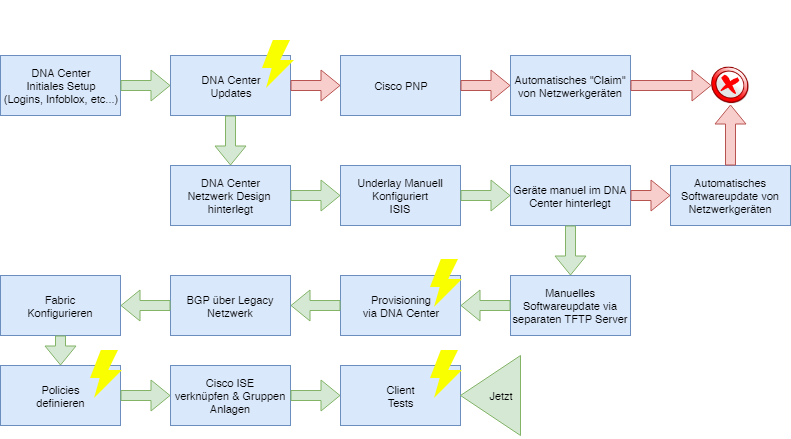
\includegraphics[height=9cm]{img/vorgehen.png}
	\caption{Grafische Übersicht über das Vorgehen beim ersten Versuch}
	\label{fig:vorgehen}
\end{figure} 

\subsection{DNA Center Initiales Setup}

\subsubsection{Installation}
\label{DNACenterSetup_Installation}
Die Installation des DNA Centers erfolgt direkt an der Konsole oder über die Cisco IMC. Dabei wird der maglev-config-wizard ausgeführt. Dieser Befehl sollte zu einem späteren Zeitpunkt nicht erneut ausgeführt werden, da er die Appliance unbrauchbar macht. 

Wie in Kapitel 2\cite{cisco-dna-installation-guide} beschrieben werden folgende Angaben benötigt:
\begin{itemize}
	\item Host IP Adresse
	\item Netmask
	\item Default Gateway IP adress
	\item DNS Servers
	\item Static Routes
	\item HTTPS Proxy
	\item Maglev Master Node IP
	\item Username, Passwort und Linux Passwort
	\item Administration Passphrase für das Web-Interface
	\item NTP Server
	\item Service Subnets
\end{itemize}

Im ersten Schritt \ref{fig:dna-center-install-step-1} wird gewählt, ob ein neuer Cluster erstellt werden soll oder einem beigetreten werden soll. Bei der Testumgebung dieser Arbeit war nur eine Appliance verfügbar, weshalb schliesslich "Start a DNA-C Cluster" ausgewählt wurde. 

\begin{figure}[H]
	\centering
	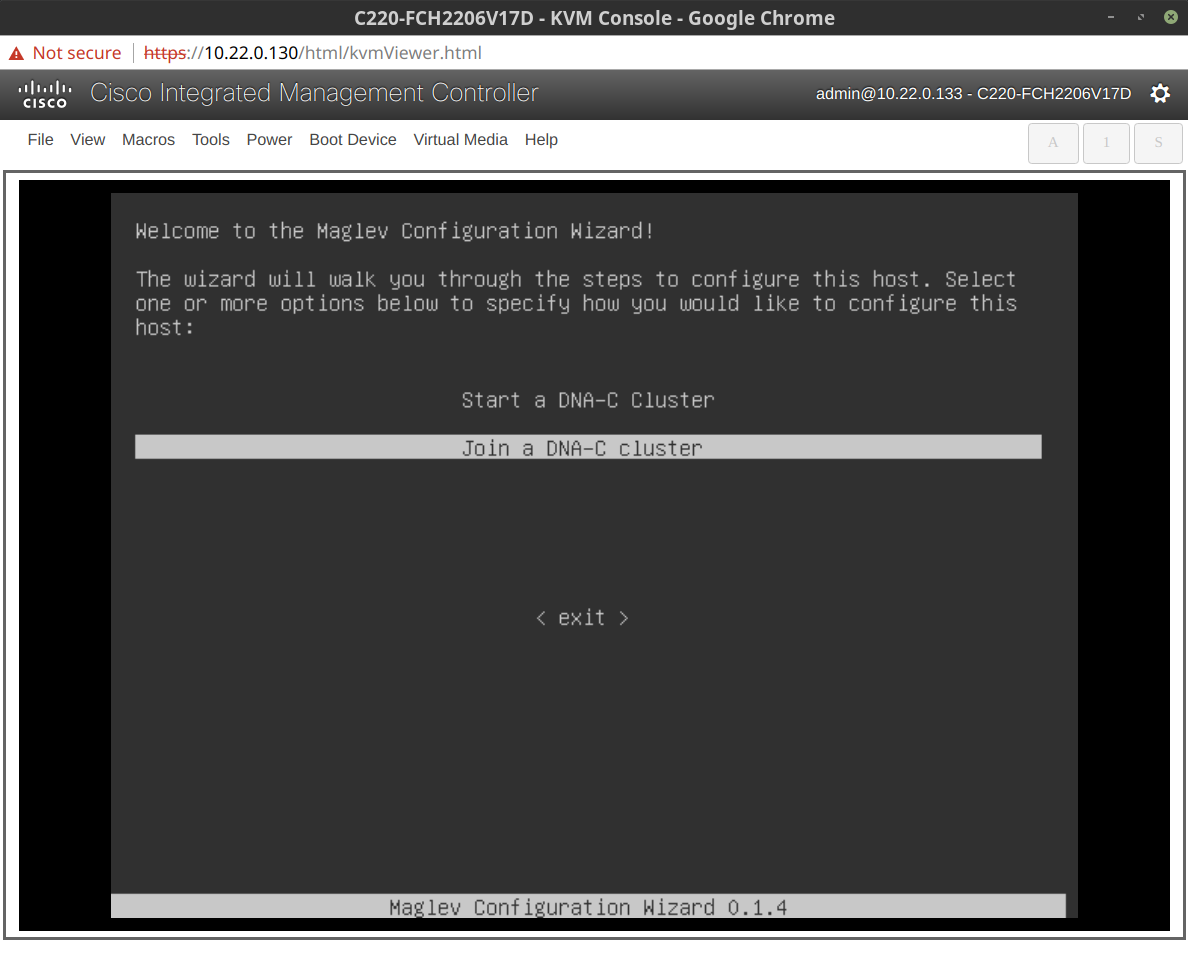
\includegraphics[height=9cm]{img/sc_001.png}
	\caption{DNA Center Configuration Wizard - Start}
	\label{fig:dna-center-install-step-1}
\end{figure} 

Im nächsten Schritt muss die IP Konfiguration für die DNA Center Appliance angegeben werden. Es muss mindestens ein Interface konfiguriert werden und als Cluster Link definiert sein. Statische Routen können definiert werden, sind aber optional.

\begin{figure}[H]
	\centering
	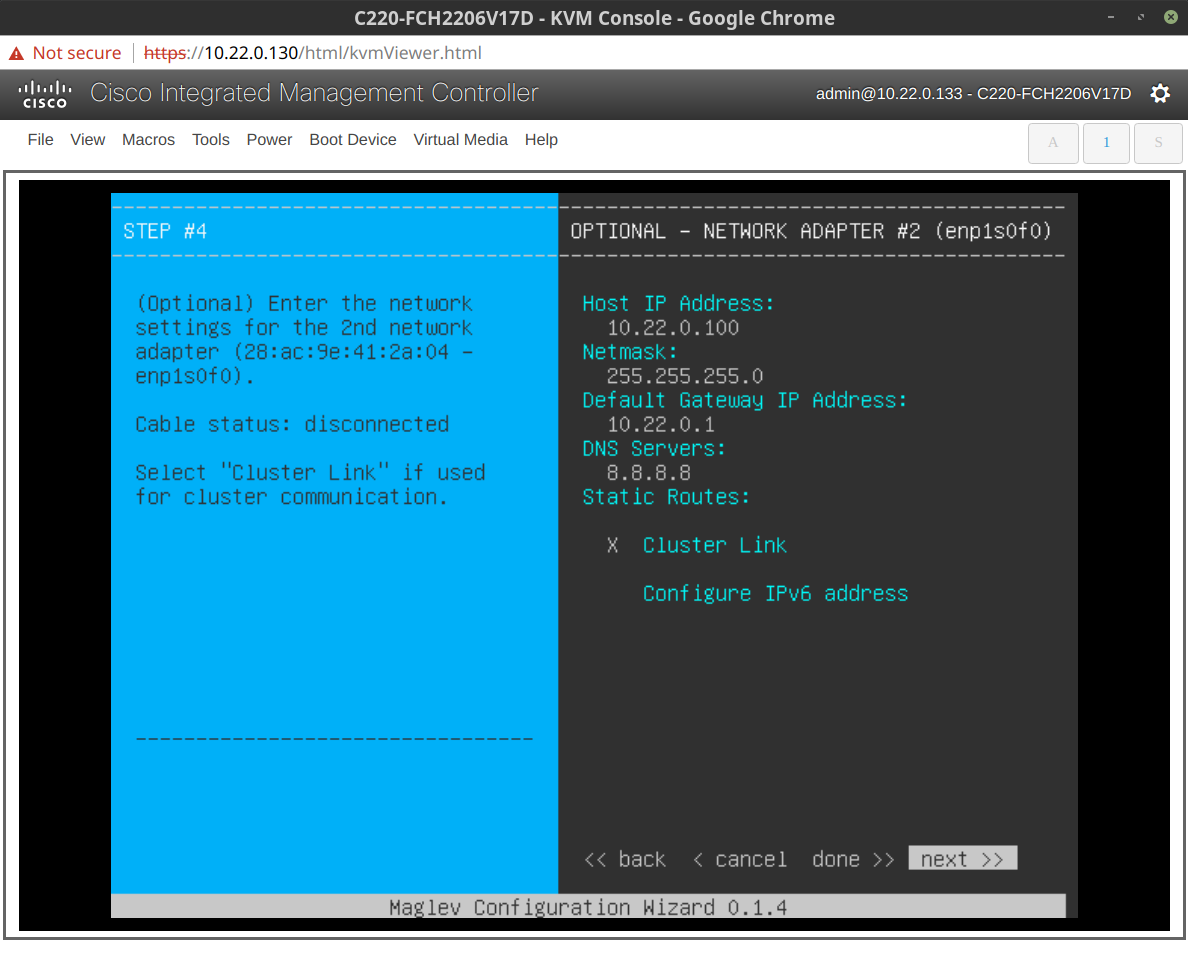
\includegraphics[height=9cm]{img/sc_002.png}
	\caption{DNA Center Configuration Wizard - Entering Management IP}
	\label{fig:dna-center-install-step-4}
\end{figure} 

Im letzten Schritt des Wizards werden alle User Account Einstellungen festgelegt. Hier bei ist zu beachten, dass das "Linux Password" für den SSH Zugriff benötigt wird und die "Administrator Passphrase" für den Zugang zum Web Interface.
 
\begin{figure}[H]
	\centering
	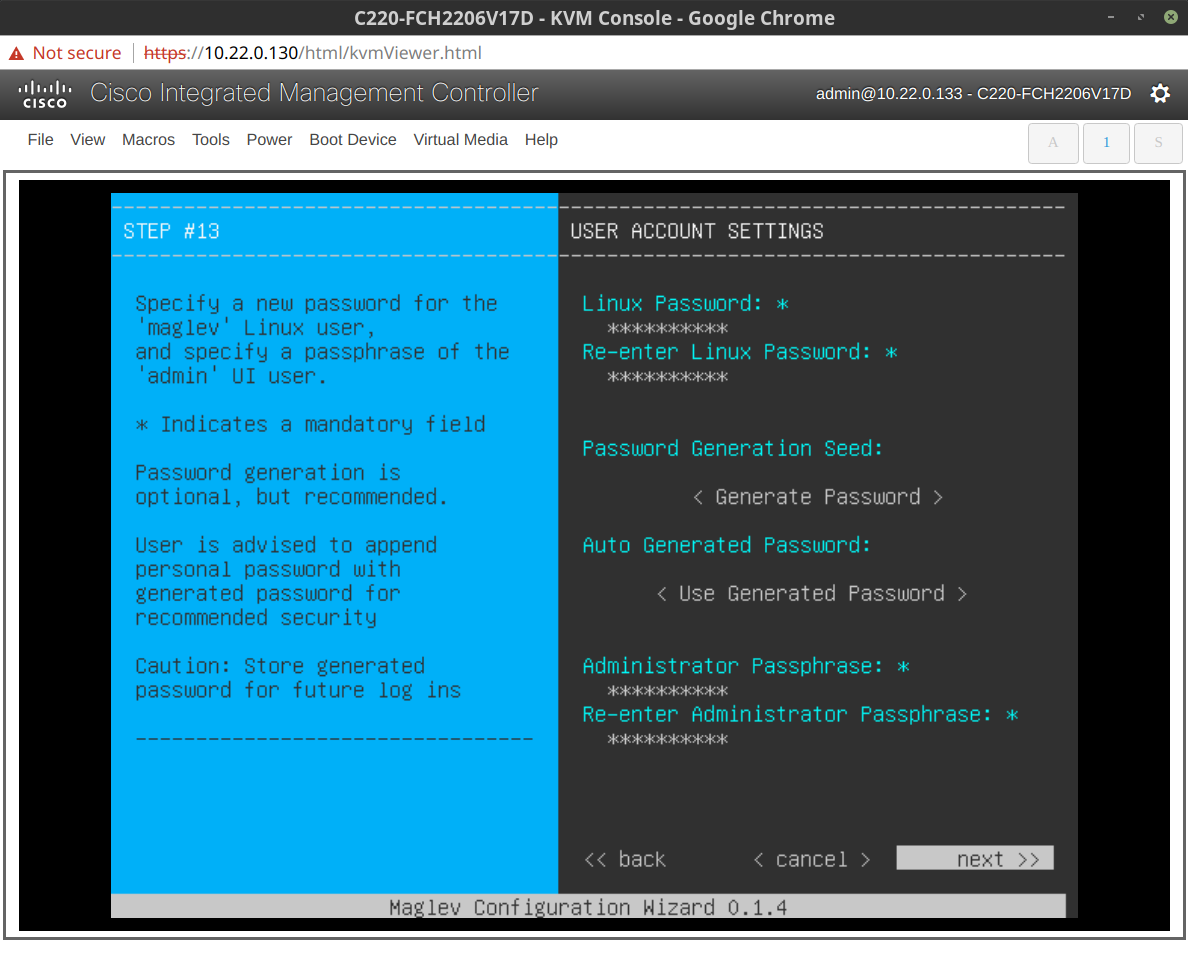
\includegraphics[height=9cm]{img/sc_003.png}
	\caption{DNA Center Configuration Wizard - Entering Authentification Data}
	\label{fig:dna-center-install-step-13}
\end{figure}

Nun wird das DNA Center aufgesetzt. Dieser Prozess dauert mehrere Stunden. 

\begin{figure}[H]
	\centering
	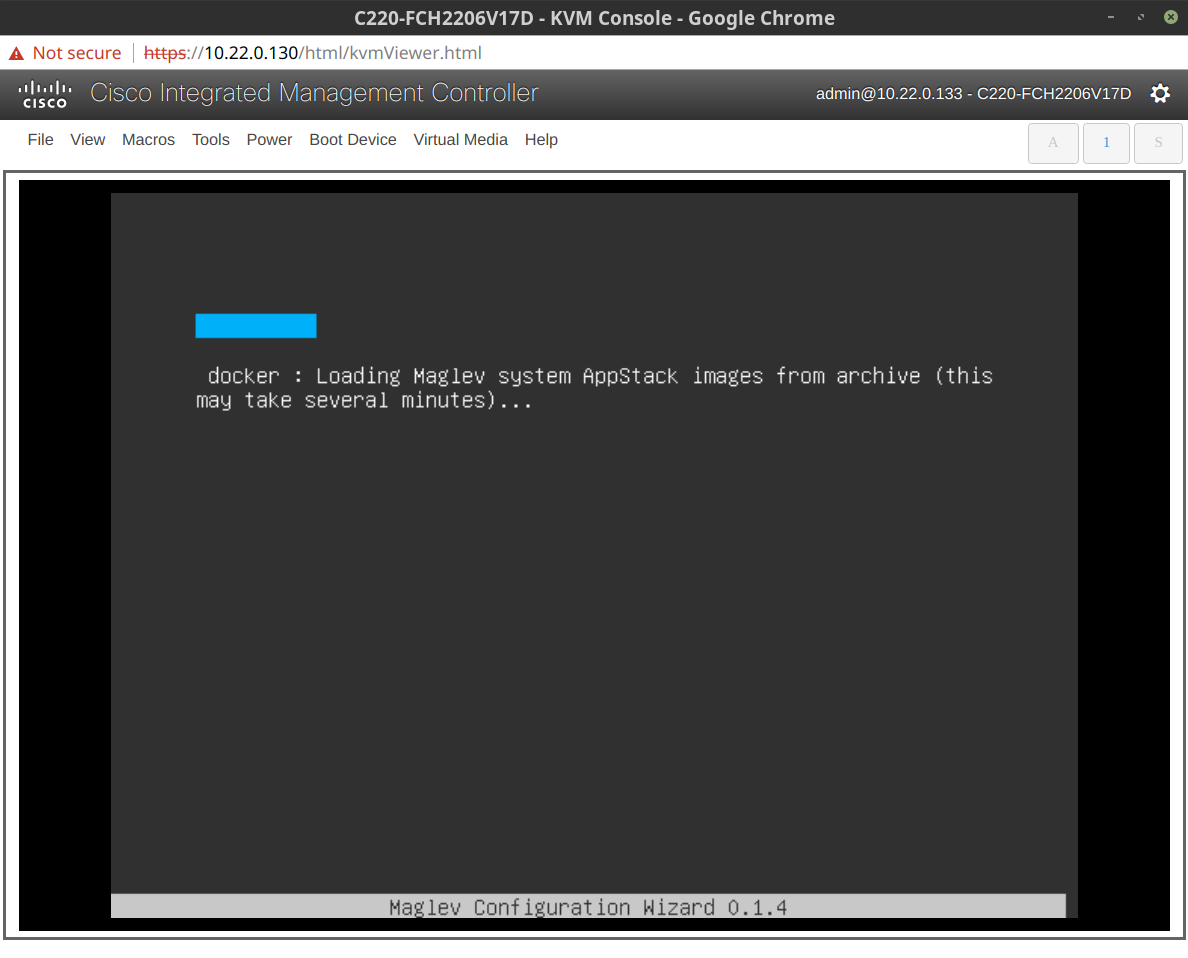
\includegraphics[height=9cm]{img/sc_004.png}
	\caption{DNA Center Configuration Wizard - DNA Center uses docker}
	\label{fig:dna-center-install-step-install}
\end{figure}


\subsubsection{Setup Accounts}
Nach dem der Wizard die Installation vollständig ausgeführt hat, ist das DNA Center Web-GUI verfügbar. Die Konfiguration kann nun über dieses weitergeführt werden.
\begin{figure}[H]
	\centering
	\includegraphics[height=9cm]{img/sc_005.png}
	\caption{DNA Center Web GUI - Login Page}
	\label{fig:dna-center-gui-1}
\end{figure}

Gleich zu Beginn verlangt das DNA Center die Cisco Credentials die mit dem Smart Account verknüpft sind, in welchem die Lizenzen verwaltet werden. Diese Informationen können auch zu einem späteren Zeitpunkt noch eingetragen werden.

\begin{figure}[H]
	\centering
	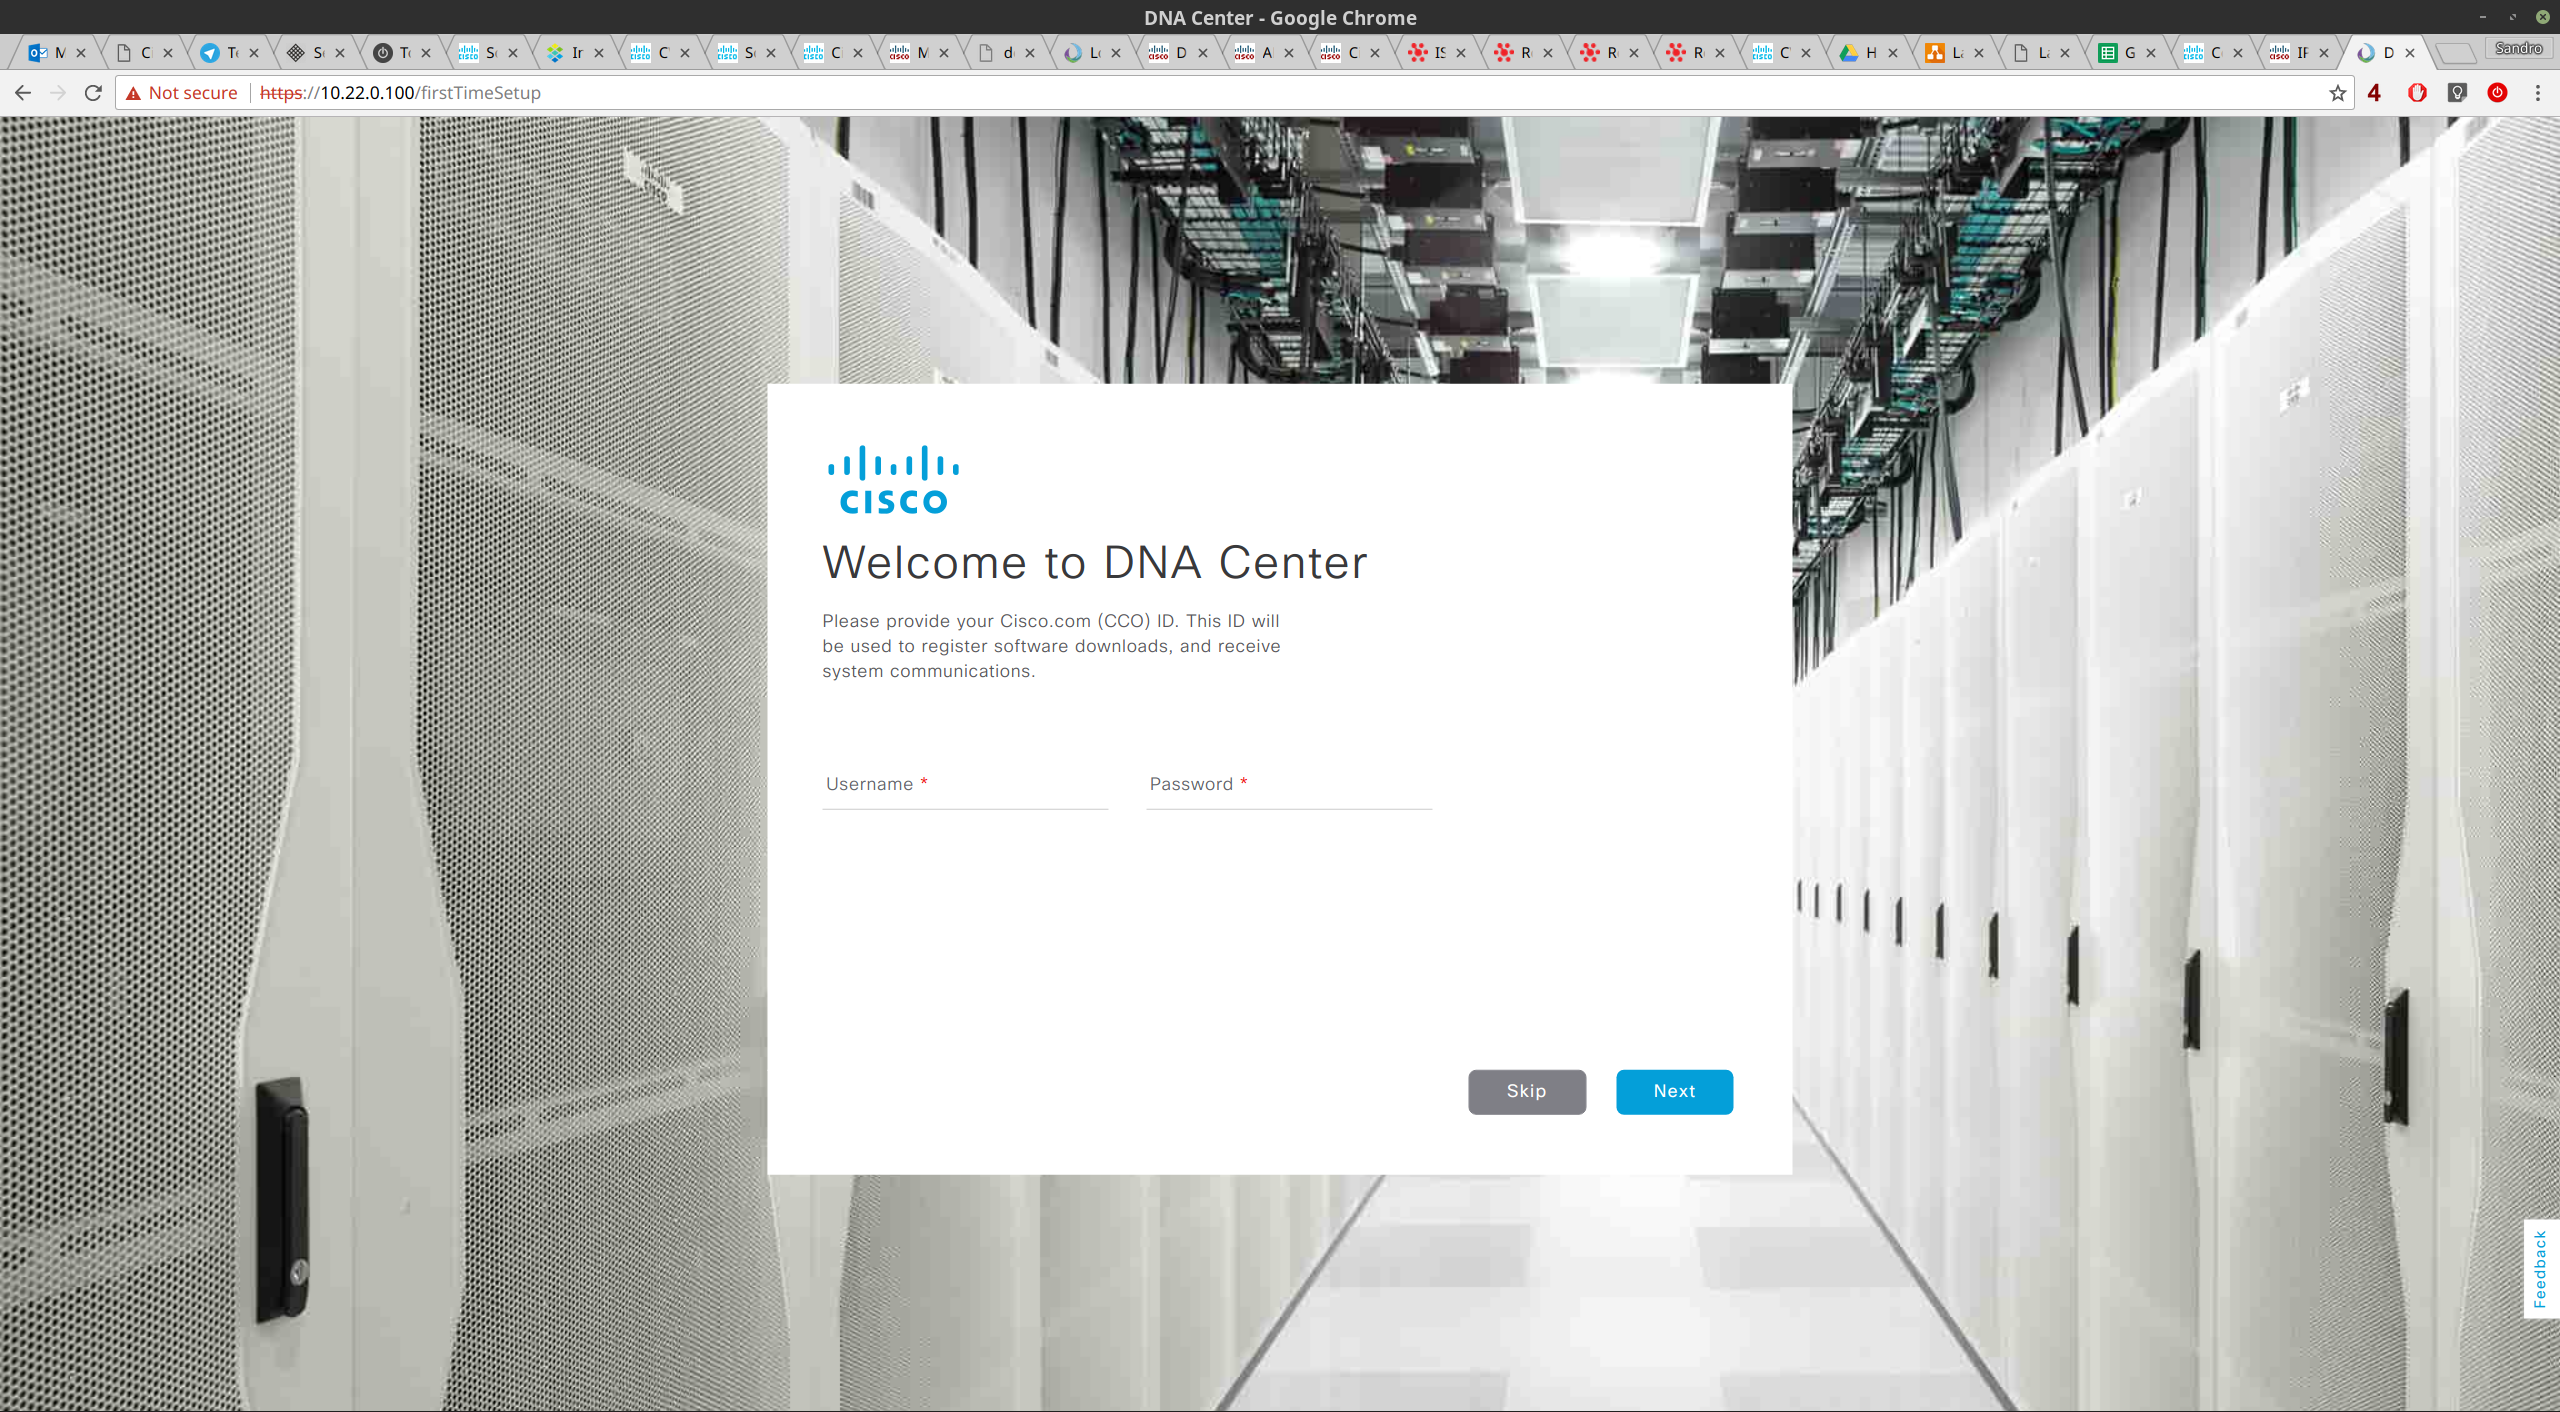
\includegraphics[height=9cm]{img/sc_006.png}
	\caption{DNA Center Web GUI - Cisco Credentials for Licences}
	\label{fig:dna-center-gui-2}
\end{figure}

Im nächsten Schritt kann ein IPAM Server angegeben werden. Diese Einstellung kann ebenfalls später angepasst werden, weshalb wir diesen Schritt zu Beginn übersprungen haben.

\begin{figure}[H]
	\centering
	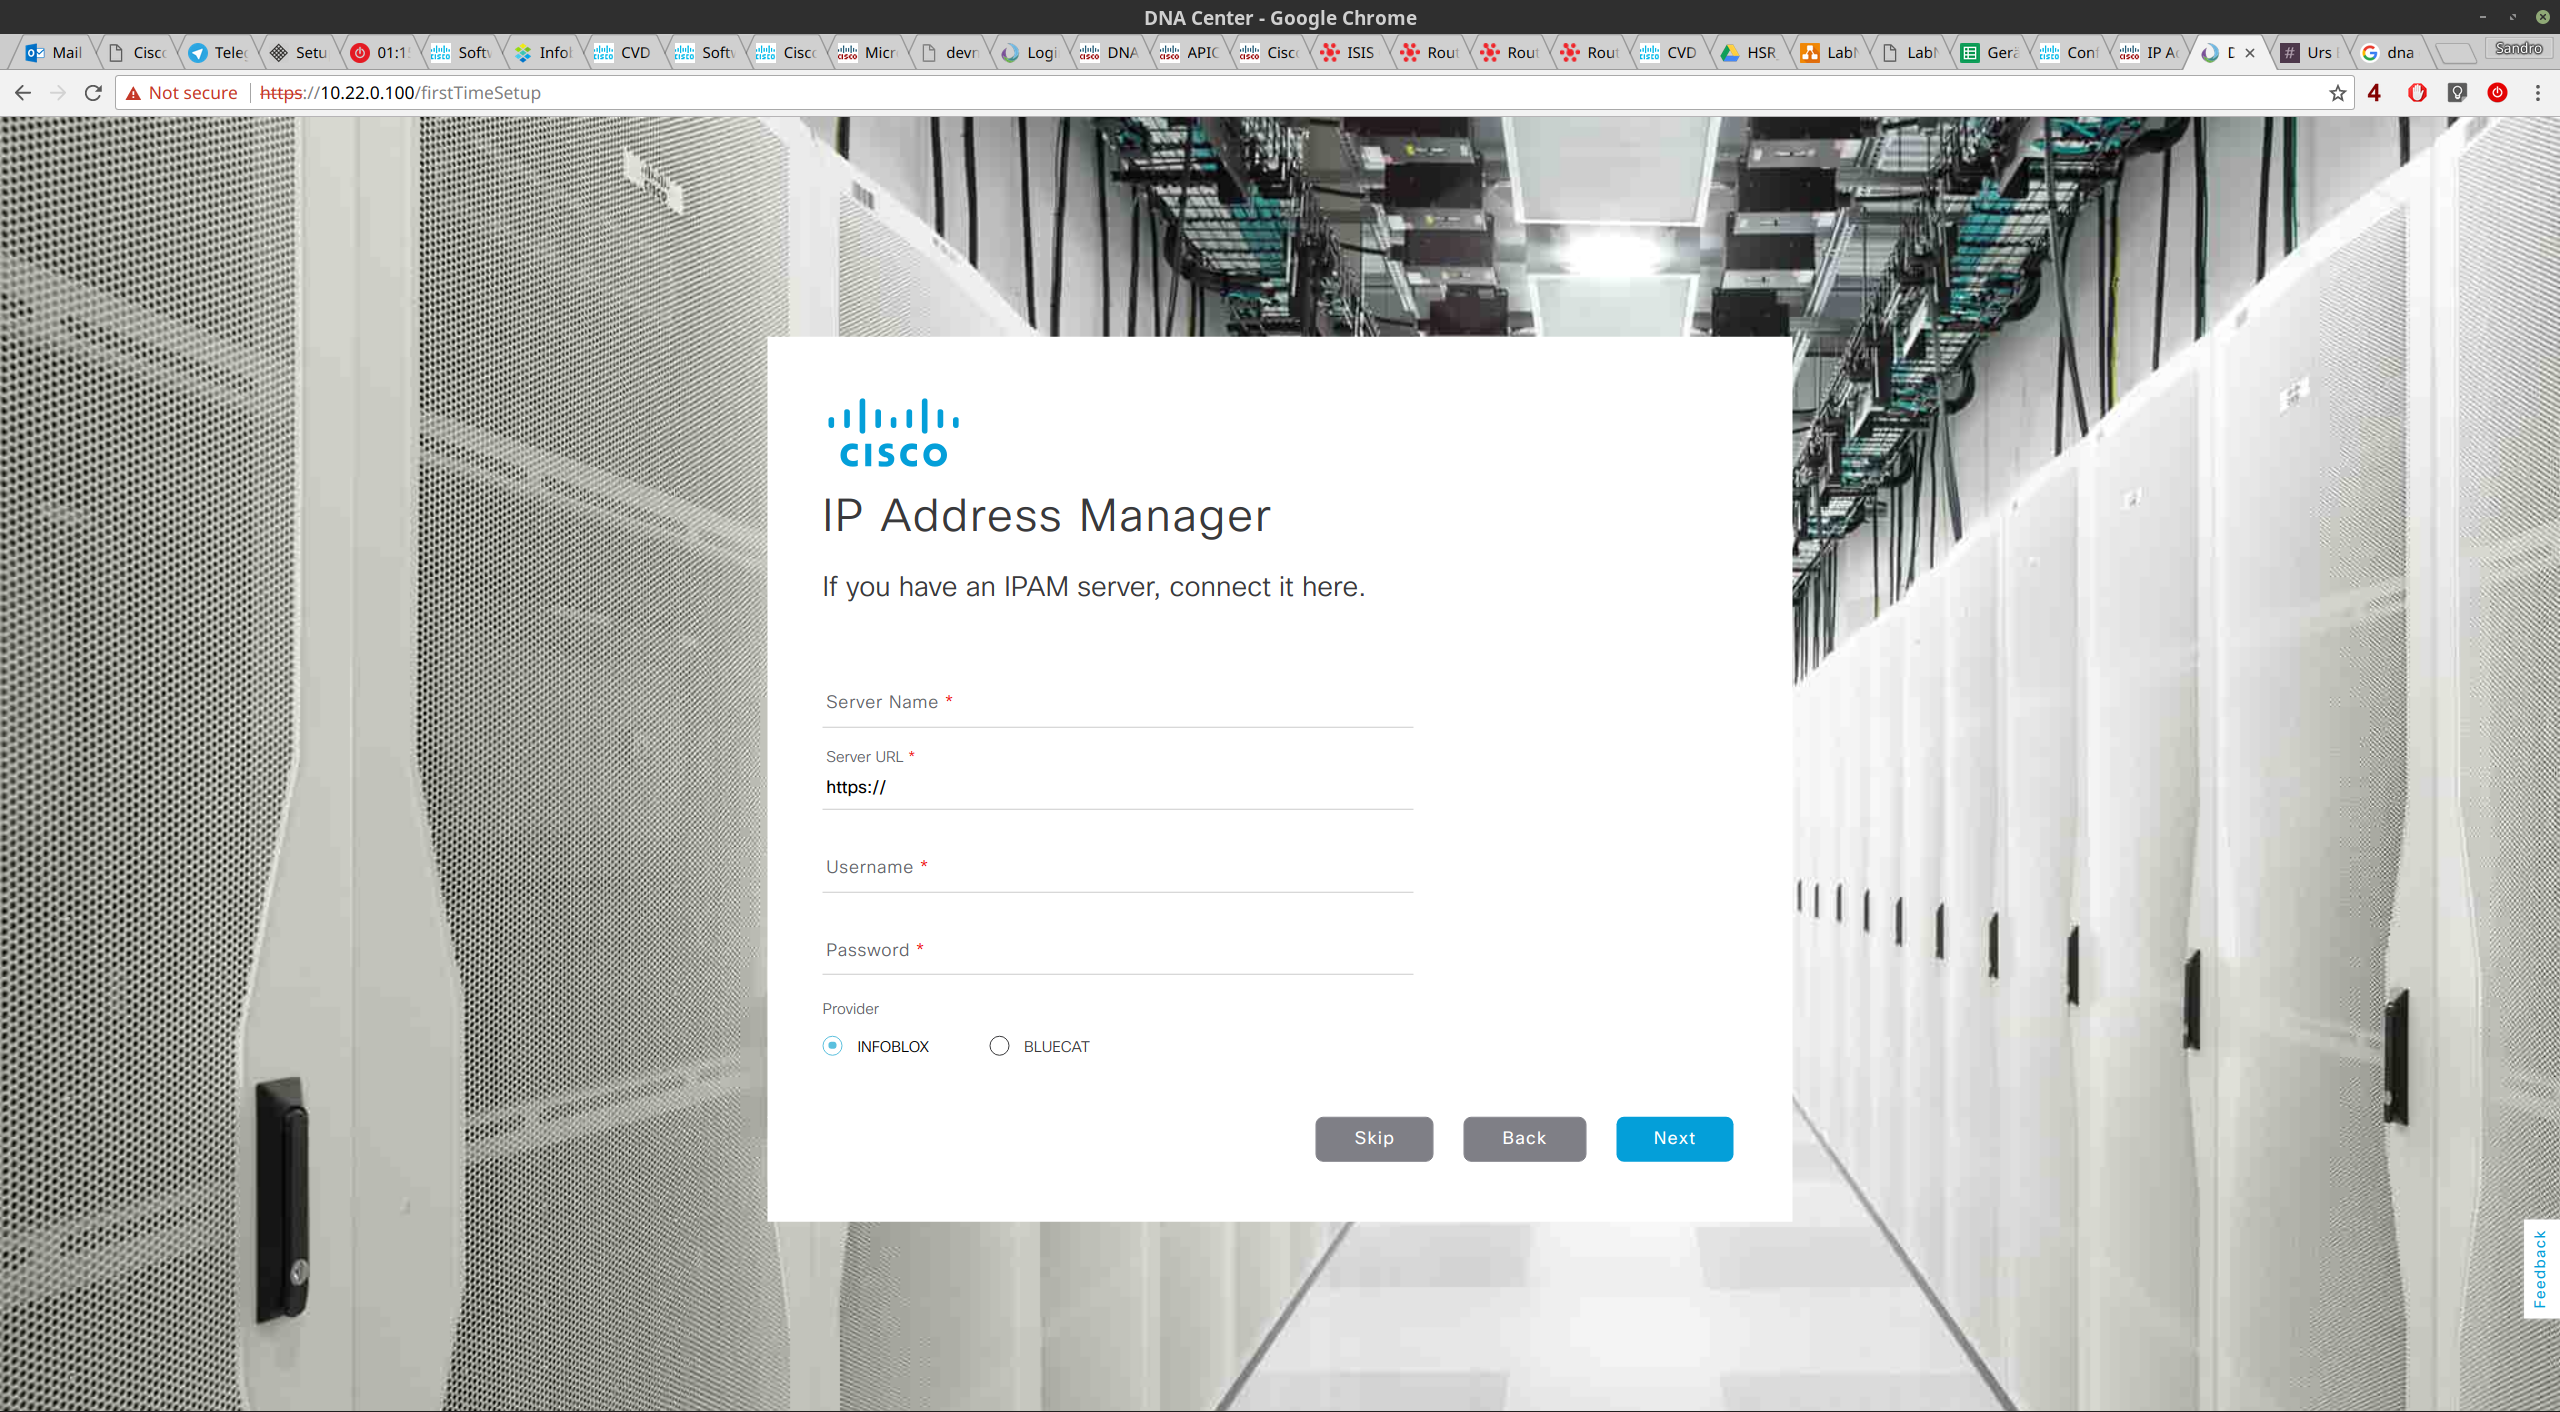
\includegraphics[height=9cm]{img/sc_007.png}
	\caption{DNA Center Web GUI - Cisco IPAM}
	\label{fig:dna-center-gui-3}
\end{figure}

Danach ist die initiale Konfiguration beendet und das DNA Center Dashboard wird angezeigt.

\begin{figure}[H]
	\centering
	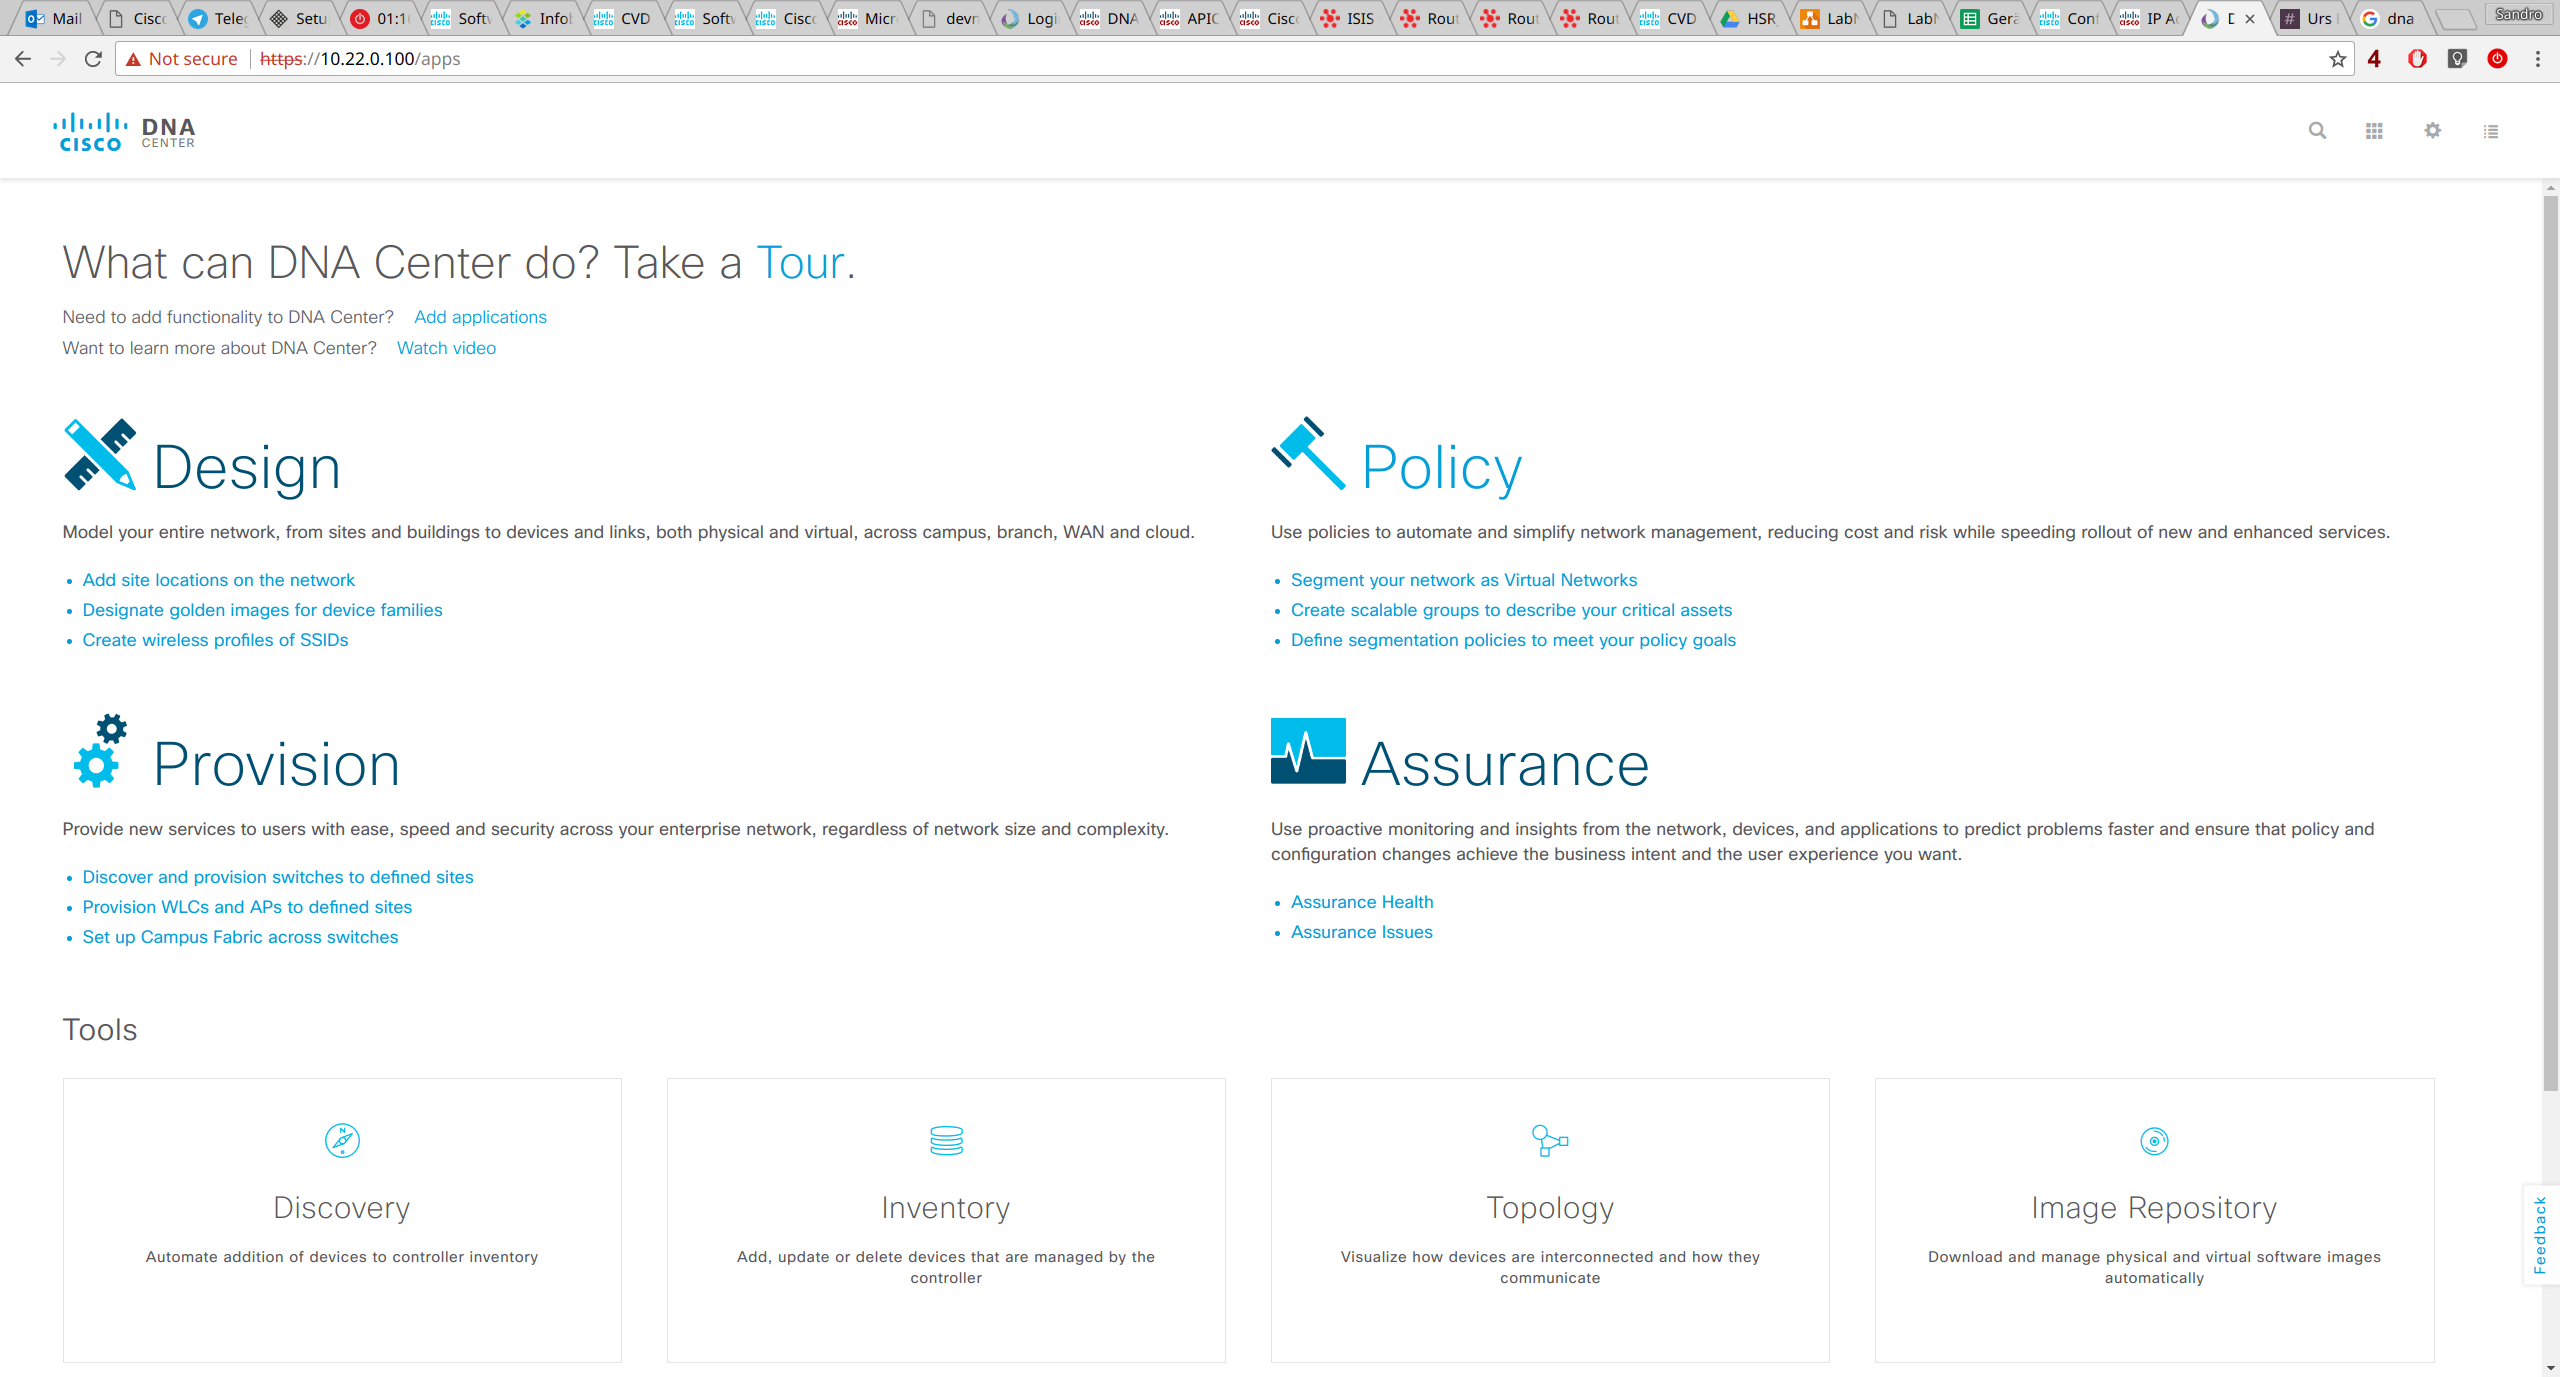
\includegraphics[height=9cm]{img/sc_008.png}
	\caption{DNA Center Web GUI - Dashboard}
	\label{fig:dna-center-gui-4}
\end{figure}

\subsection{DNA Center Updates}
\label{DNACenter_Updates}
Da sich das DNA Center während dem Setup Prozess nicht automatisch aktualisiert und die DNA Center Versionen in relativ kurzen Intervallen released werden, ist es ratsam, gleich zu Beginn die aktuellsten Updates zu installieren.

Der Updateprozess birgt jedoch einige Hürden:
\begin{itemize}
	\item System Updates müssen vor den Package Updates heruntergeladen und installiert werden.
	\subitem Werden die Package Updates vor dem System Update ausgeführt, können diese blockieren. 
	\item Die Package Updates müssen in der richten Reihenfolge installiert werden.
	\item Die oben genannte Reihenfolge ist nicht direkt ersichtlich.
	\item Der Updatevorgang dauert mehrere Stunden.
	\item Der Updatefortschritt wird nicht angezeigt. 
	\item Während dem Updateprozess können Teile des Web-GUIs Fehlermeldungen anzeigen oder überhaupt nicht mehr erreichbar sein.\\
\end{itemize} 

Die Update Ansicht ist unter \textit{Einstellungen (Zahnrad-Symbol) $\rightarrow$ System Settings  $\rightarrow$ App Management} zu finden:

\begin{figure}[H]
	\centering
	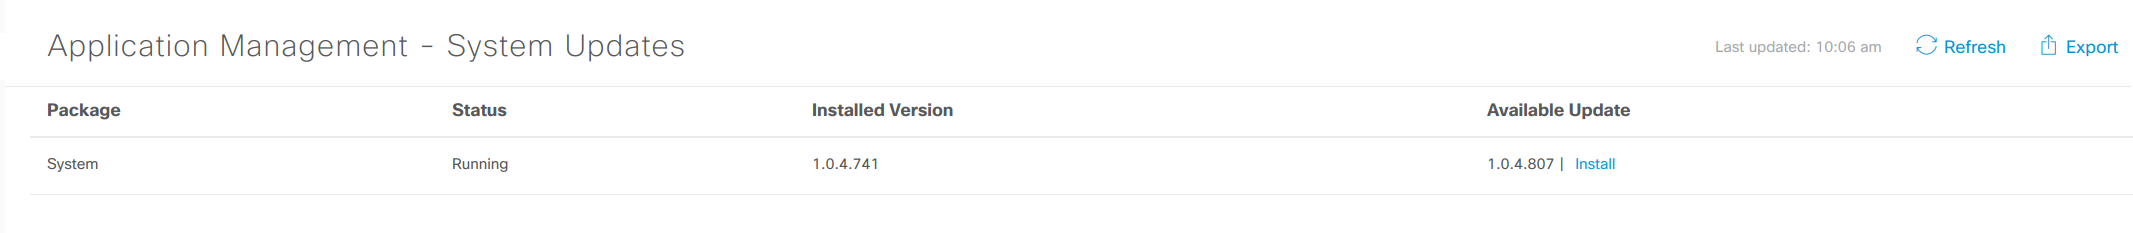
\includegraphics[width=\columnwidth]{img/sc_009.png}
	\caption{DNA Center App Management}
	\label{fig:dna-center-gui-update-1}
\end{figure}

\subsubsection{Fehlgeschlagene Updates reparieren}
Falls Updates in der falschen Reihenfolge installiert wurden oder aus anderen Gründen blockiert sind, können bereits heruntergeladene oder installierte Updates mit folgenden Befehlen entfernt und bereinigt werden.
(am Beispiel von main-system-package:1.0.4.779):

\begin{lstlisting}[language=bash]
$ maglev package status | awk  '$3 ~ /[0-9]+/ {print $1":"$3}' | 
grep -v "^system" |  while read pkg; 
do maglev catalog package delete $pkg;done
$ maglev system_update_package install main-system-package:1.0.4.779
\end{lstlisting}

\subsubsection{Update Reihenfolge}
Nach einem Update wurde die Reihenfolge von System und Package Updates angepasst. Vermutlich um den Administrator dazu zu bringen zuerst die System Updates zu installieren. 

\begin{figure}[H]
	\centering
	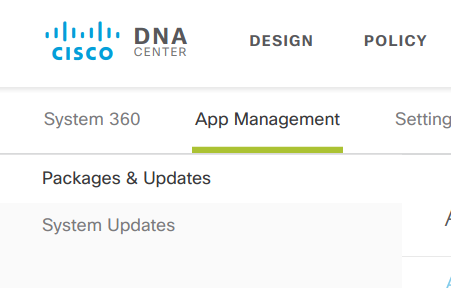
\includegraphics[height=4cm]{img/sc_010.png}
	\caption{DNA Center App Management - Alte Menü Anordnung}
	\label{fig:dna-center-gui-update-2}
\end{figure}

\subsubsection{Schwierigkeit: CCO Credentials für Updates notwendig}

Application Packages und System Updates können nur installiert werden, wenn die CCO Credentials hinterlegt sind.

\begin{figure}[H]
	\centering
	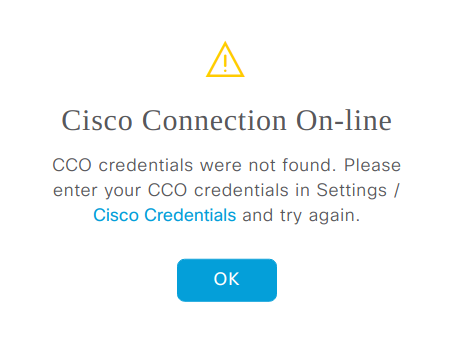
\includegraphics[height=4cm]{img/dan-center-cisco-credentials-required.png}
	\caption{DNA Center Upgrade - Cisco Credentials required}
	\label{fig:dna-center-cisco-credentials-required}
\end{figure}

\subsubsection{Schwierigkeit: Unterschiedliche Versionsangabe}

Beim Updatevorgang kann es zu Verwirrungen kommen, weil die Versionangabe von der Funktion \textit{About} von der Version des System Packages abweicht.

\begin{figure}[H]
	\centering
	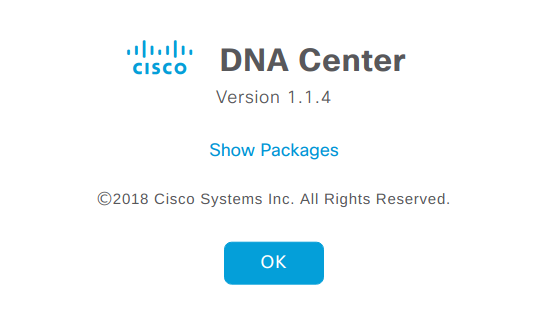
\includegraphics[height=3cm]{img/dna-center-about.png}
	\caption{DNA Center - About - Version}
	\label{fig:dna-center-about}
\end{figure}

Oben wurde bei \textit{About} die richtige Version 1.1.4 angegeben. Nachfolgend die Anzeige unter \textit{System Updates}, welche eine andere Version anzeigt.
\begin{figure}[H]
	\centering
	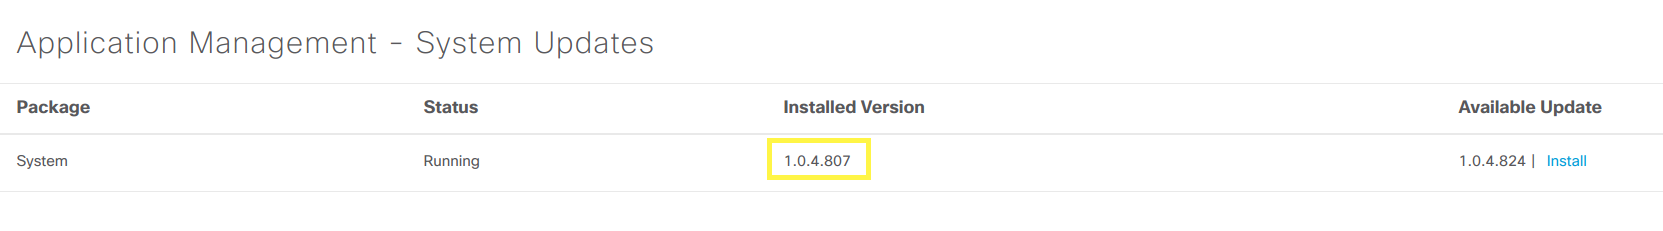
\includegraphics[height=2.25cm]{img/dna-center-system-upgrade-version.png}
	\caption{DNA Center - System Upgrade - Version}
	\label{fig:dna-center-system-upgrade}
\end{figure}

\subsection{DNA Center Netzwerk Design}
\label{DNACenterNetwork_Design}
\subsubsection{Network Hierarchy}

Gemäss unserer Netzwerk Architektur wie in Kapitel \ref{fig:LabNetworkArchitecture} beschrieben, haben wir zwei Standorte. Rapperswil mit zwei Gebäuden und Jona mit einem Gebäude.
In DNA Center können diese sehr einfach im Abschnitt \textit{Design $\rightarrow$ Network Hierarchy} hinzugefügt werden. 

\begin{figure}[H]
	\centering
	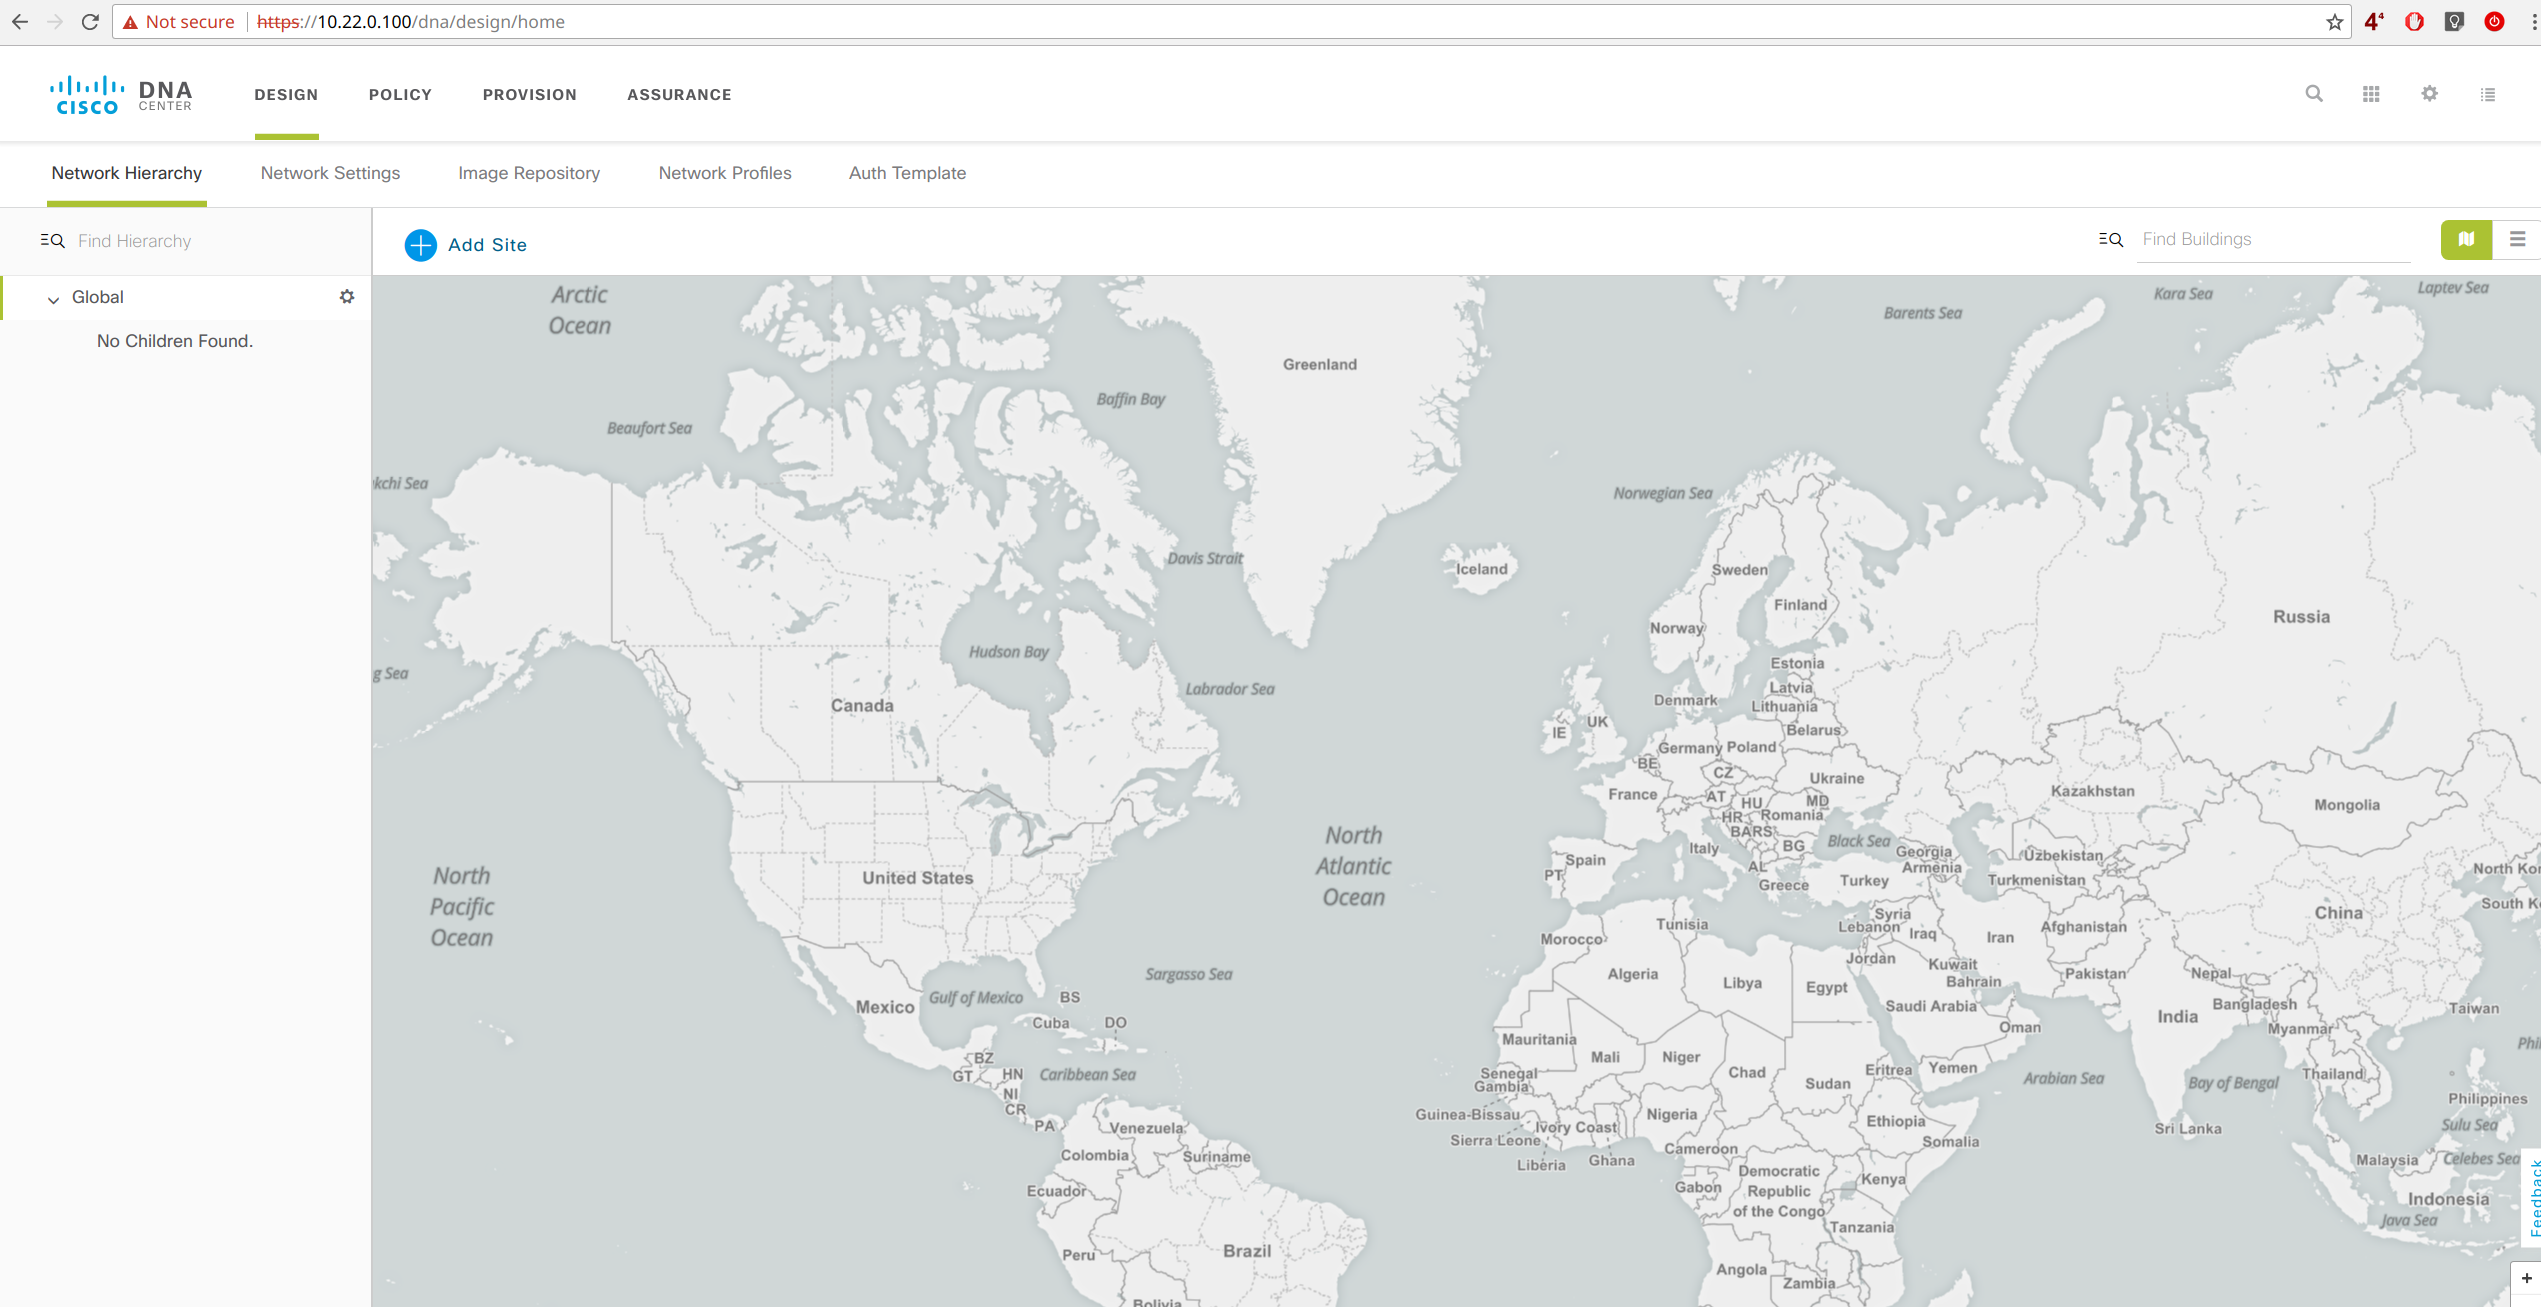
\includegraphics[height=8cm]{img/Selection_011.png}
	\caption{DNA Center Design Map}
	\label{fig:dna-center-design-1}
\end{figure}

\begin{figure}[H]
	\centering
	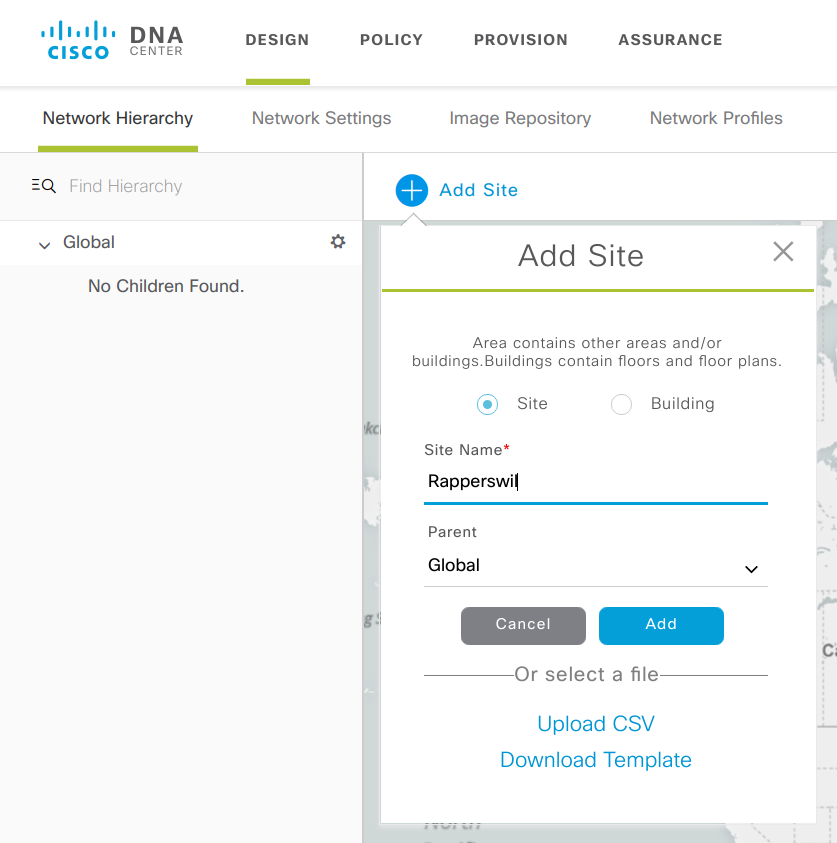
\includegraphics[height=6cm]{img/Selection_012.png}
	\caption{DNA Center Design - Standort hinzufügen}
	\label{fig:dna-center-design-2}
\end{figure}

\begin{figure}[H]
	\centering
	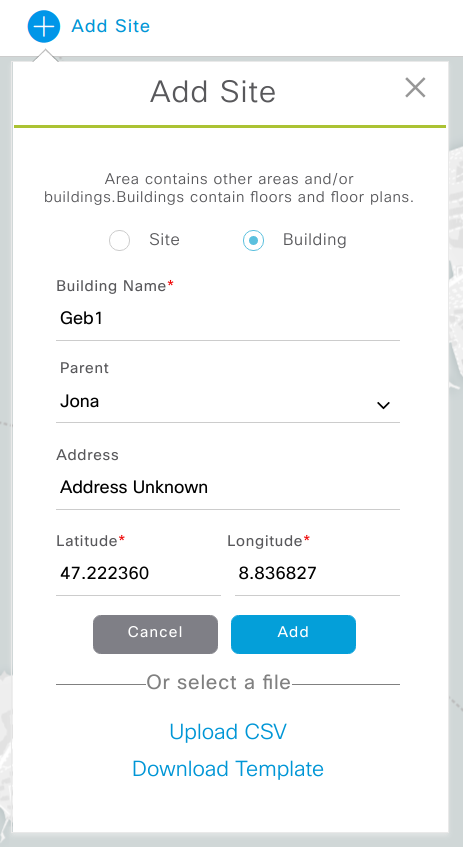
\includegraphics[height=6cm]{img/Selection_014.png}
	\caption{DNA Center Design - Gebäude können mit Koordinaten hinzugefügt werden.}
	\label{fig:dna-center-design-3}
\end{figure}

\begin{figure}[H]
	\centering
	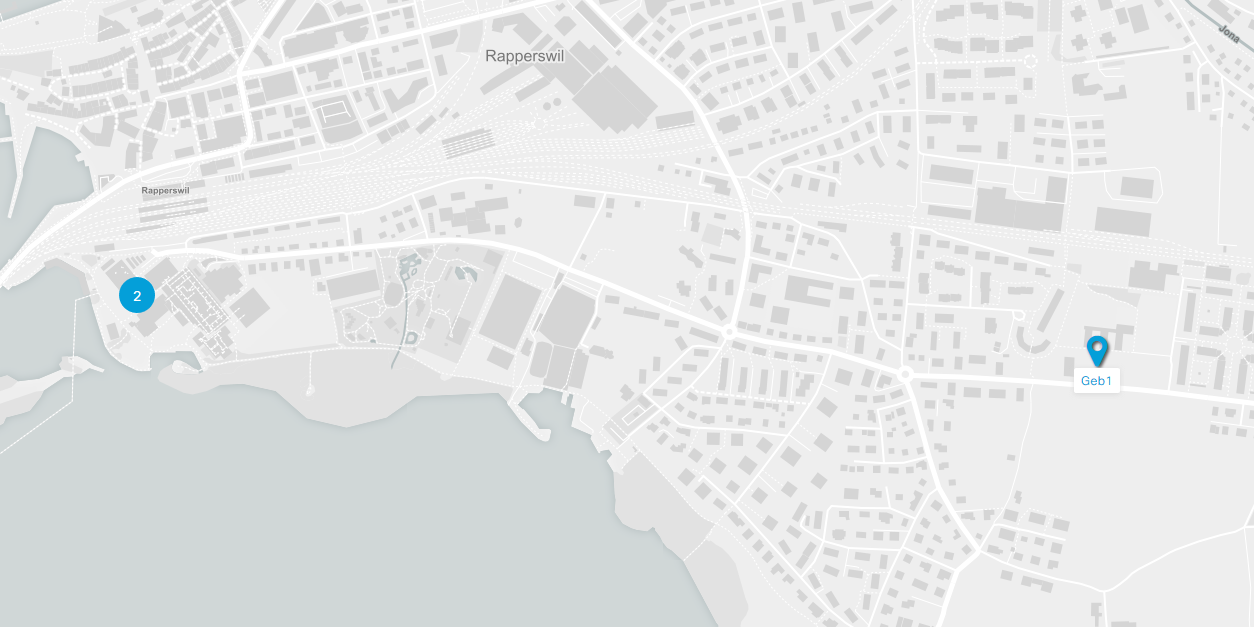
\includegraphics[height=8cm]{img/design_map_overview.PNG}
	\caption{DNA Center Design - Übersicht über alle Standorte und Gebäude}
	\label{fig:dna-center-design-overview}
\end{figure}

\subsection{LAN Automation}
Das DNA Center nutzt Plug and Play um automatisch Netzwerkgeräte in Betrieb zu nehmen und initial zu konfigurieren.
 
\subsubsection{DHCP Konfiguration}
Bei unserem ersten Versuch ein Seed-Device festzulegen, wurde vom DNA Center kein DHCP Server konfiguriert, weshalb wir diesen manuell auf Infoblox eingerichtet haben.\\


Cisco PnP kann über die DHCP Optionen 43 und 60 konfiguriert werden ( \cite{cisco-pnp-dhcp}). In unserem Fall haben wir diese Optionen wie nachfolgend auf der Grafik erischtlich auf dem Infoblox Server konfiguriert. Diese sind nötig, damit das Netzwerkgerät den PnP Server findet.

\begin{figure}[H]
	\centering
	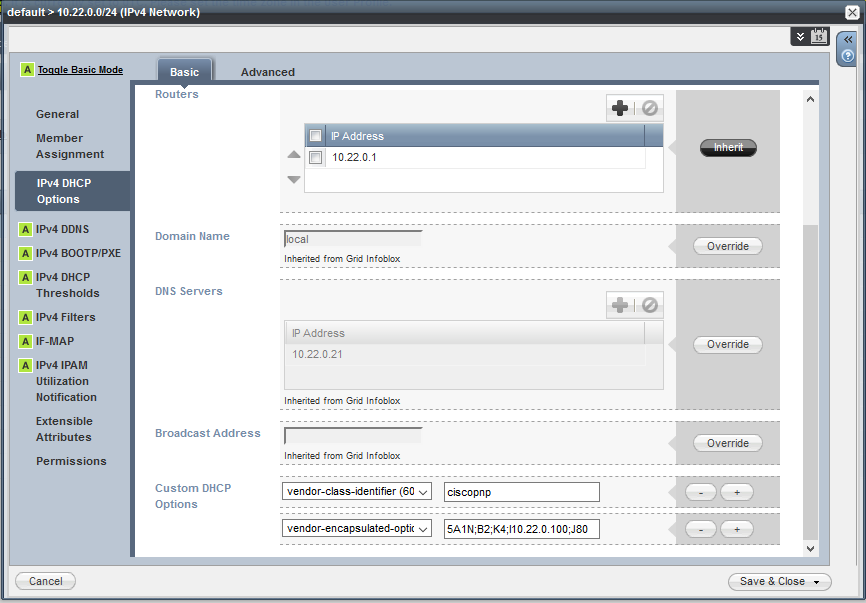
\includegraphics[height=10cm]{img/Infoblox_PNP.png}
	\caption{Infoblox Cisco PNP DHCP Option Konfiguration}
	\label{fig:cisco-pnp}
\end{figure}

Mit diesen Einstellungen hat PnP funktioniert. Allerdings nur sehr unzuverlässig und es kam oft zu Problemen, weshalb dies für viele Geräte mehrmals wiederholt werden musste. Hier ist zu empfehlen, nie mehr als ein Gerät gleichzeitig in Betrieb zu nehmen, damit es möglichst wenig Probleme gibt.

\begin{figure}[H]
	\centering
	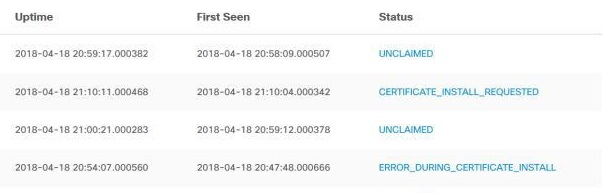
\includegraphics[height=4cm]{img/DNA_Center_Unclaimed_Errors_1.PNG}
	\caption{DNA Center Provision - Fehlermeldungen in der "Unclaimed List"}
	\label{fig:dna-center-provision-unclaimed-2}
\end{figure}
\subsection{Underlay Konfiguration}

Das ISIS Routing im Underlay sollte vom DNA Center automatisch konfiguriert werden können. Da die entsprechende Funktion LAN Automation in unserem Versuch aber nicht funktionierte, wurde der Underlay manuell konfiguriert. Dazu wurden auf den Geräten IP Addressen auf den Loopback Interfaces und den P2P Links konfiguriert und entsprechende Router eingerichtet. Am Border wurde BGP verwendet, damit die Devices auch aus dem Legacy Netz erreichbar sind.\\
Dabei ist uns aufgefallen, dass die Geräte nur über eine IP-Base Lizenz verfügen. Für die Verwendung von BGP und VRF-lite ist aber die IP-Services Lizenz nötig. 

\begin{figure}[H]
	\centering
	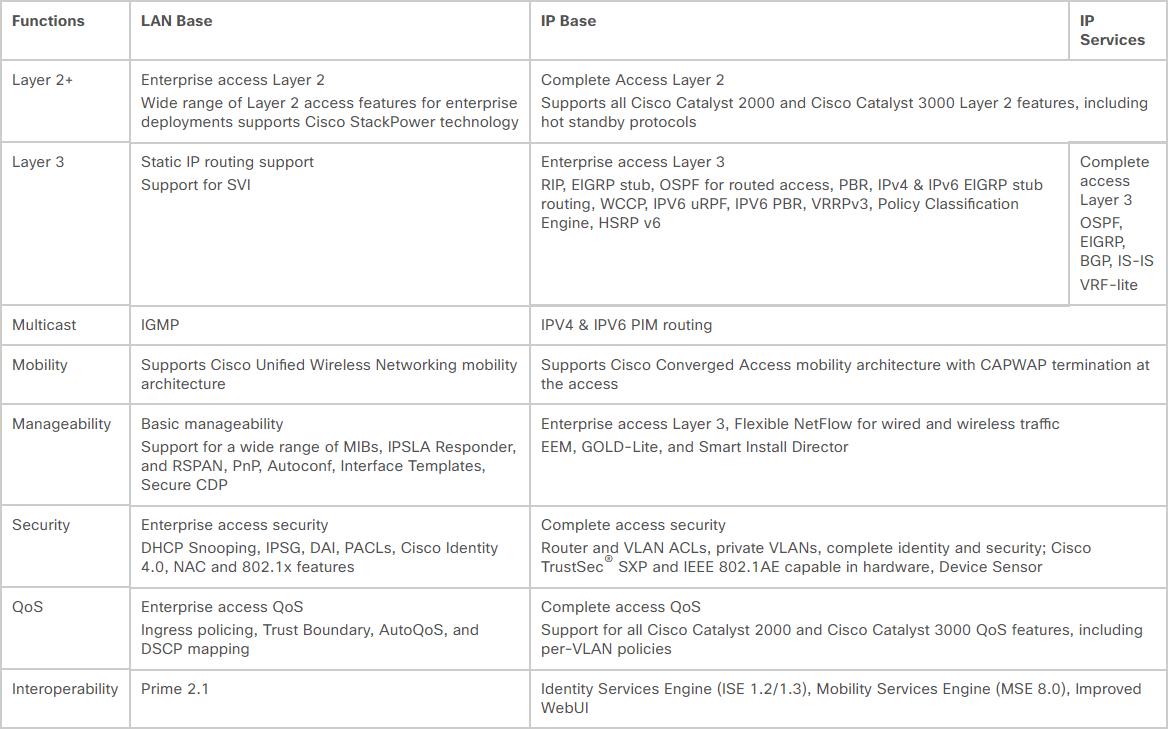
\includegraphics[width=16cm]{img/IPBaseServices.png}
	\caption{IP Base and Services}
	\label{fig:IP Base and Services Licences}
\end{figure}

Mit folgenden Befehlen war es möglich, eine IP-Services Test Lizenz zu aktivieren und somit die benötigten Features zu nutzen.

\begin{lstlisting}[language=bash]
sh license right-to-use activate ipservices all accepptEULA
reload
show license right-to-use
\end{lstlisting}

\subsection{"Claim" von Netzwerkgeräten}

\subsubsection{DNA Center Provision - Unclaimed Devices}

Nachdem die Geräte via PnP eine initiale Konfiguration erhalten haben und die Konnektivität via ISIS und BGP sichergestellt war, wurden diese im Device Inventory als Unclaimed Devices angezeigt.

\begin{figure}[H]
	\centering
	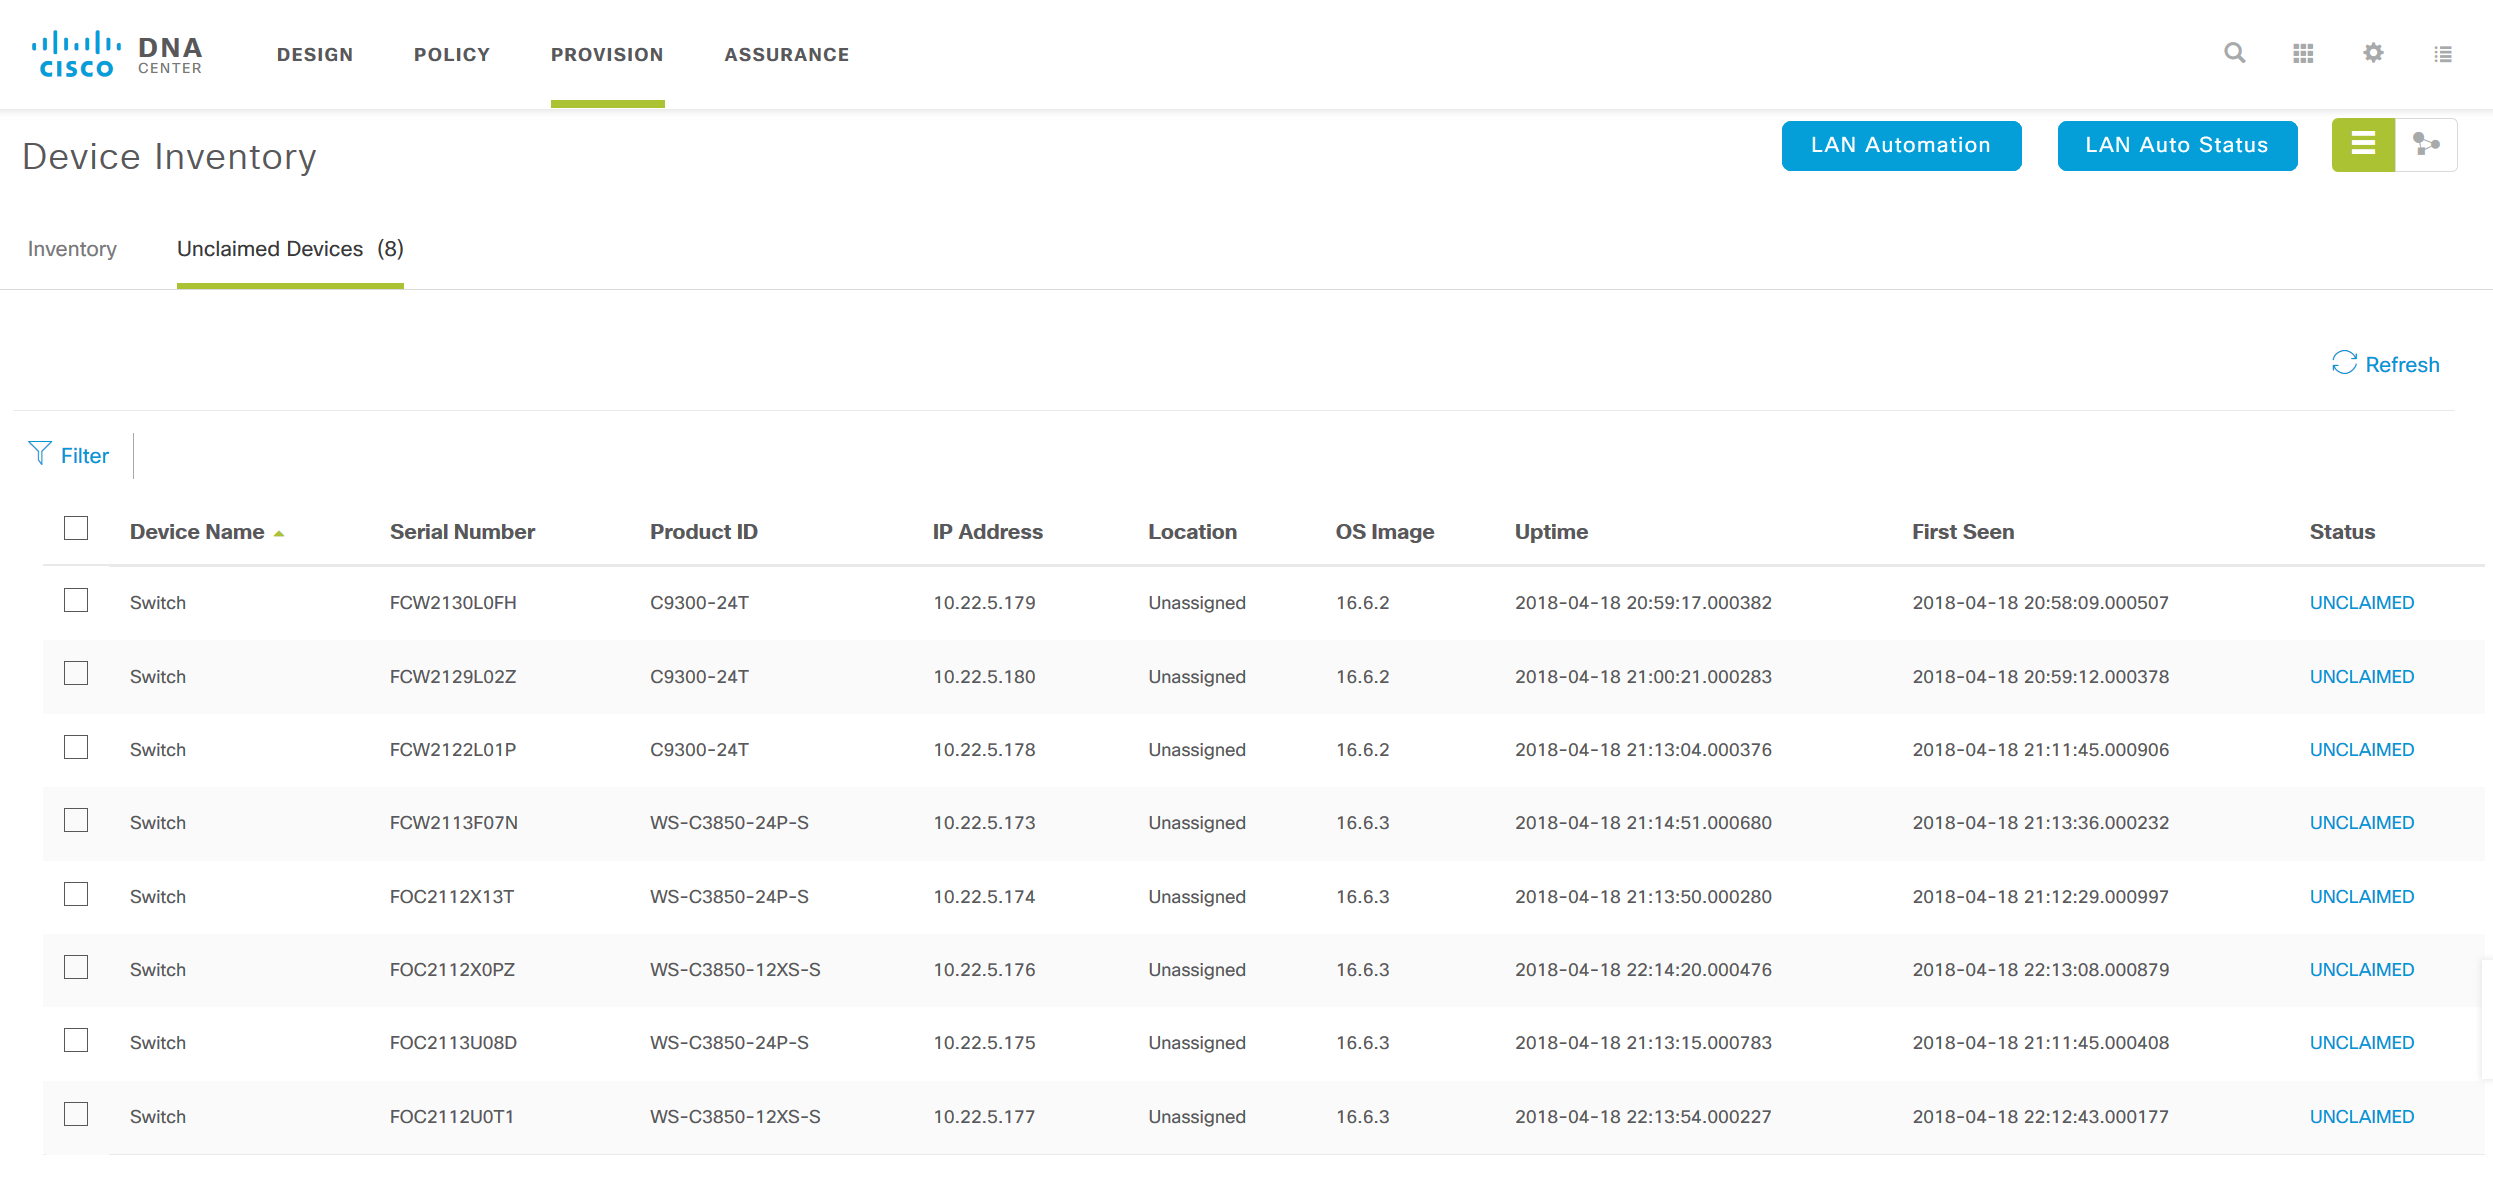
\includegraphics[height=8cm]{img/DNA_Center_All_Fabric2_Unclaimed.PNG}
	\caption{DNA Center Provision - Alle Geräte erfolgreich in der "Unclaimed List"}
	\label{fig:dna-center-provision-unclaimed}
\end{figure} 


\subsection{Netzwerkgeräte zu Inventory hinzufügen}

Der nächste Schritt wäre nun, die Devices zu "Claimen". Dies bedeutet, dass die Geräte einem Standort zugewiesen werden und somit erste Konfigurationen erhalten können. Der Claim Prozess hat leider gar nie funktioniert. Das DNA Center reagierte einfach nicht auf die Eingabe.

\subsubsection{Manuell Geräte im DNA Center hinzufügen}
Da alle Versuche die Geräte automatisch hinzuzufügen gescheitert sind, entschieden wir uns den Vorgang manuell durchzuführen. 

Im Dashboard klickt man dazu auf \textit{Inventory} (siehe \ref{fig:dna-center-inventory-button})

\begin{figure}[H]
	\centering
	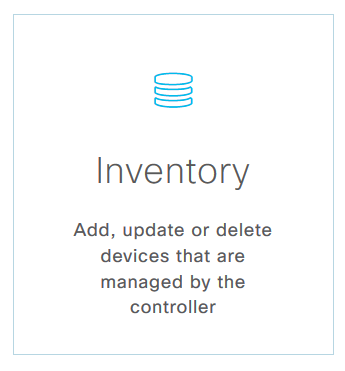
\includegraphics[height=3cm]{img/dna-center-inventory-button.PNG}
	\caption{DNA Center Dashboard - Inventory Knopf}
	\label{fig:dna-center-inventory-button}
\end{figure}

Anschliessend wählt man \textit{Add} (siehe \ref{fig:dna-center-inventory-add})

\begin{figure}[H]
	\centering
	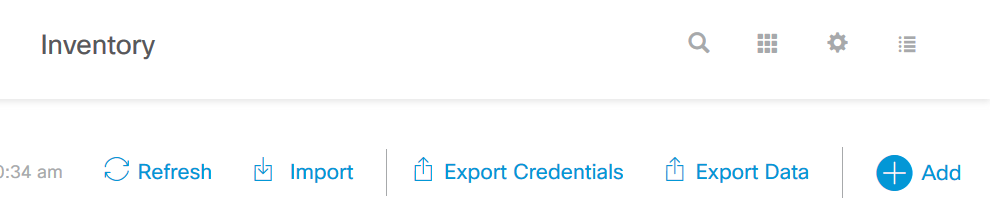
\includegraphics[height=3cm]{img/dna-center-inventory-add.PNG}
	\caption{DNA Center Inventory - Gerät hinzufügen}
	\label{fig:dna-center-inventory-add}
\end{figure}

Danach müssen folgende Informationen eingegeben werden:

\begin{itemize}
	\item Device Type
	\item Device IP \ Name
	\item SNMP (Version, Read und Write Community)
	\item CLI (via SSH oder Telnet) \textit{oder}
	\item NETCONF
\end{itemize}

Wir entschieden uns hier CLI via SSH zu wählen.

\begin{figure}[H]
	\centering
	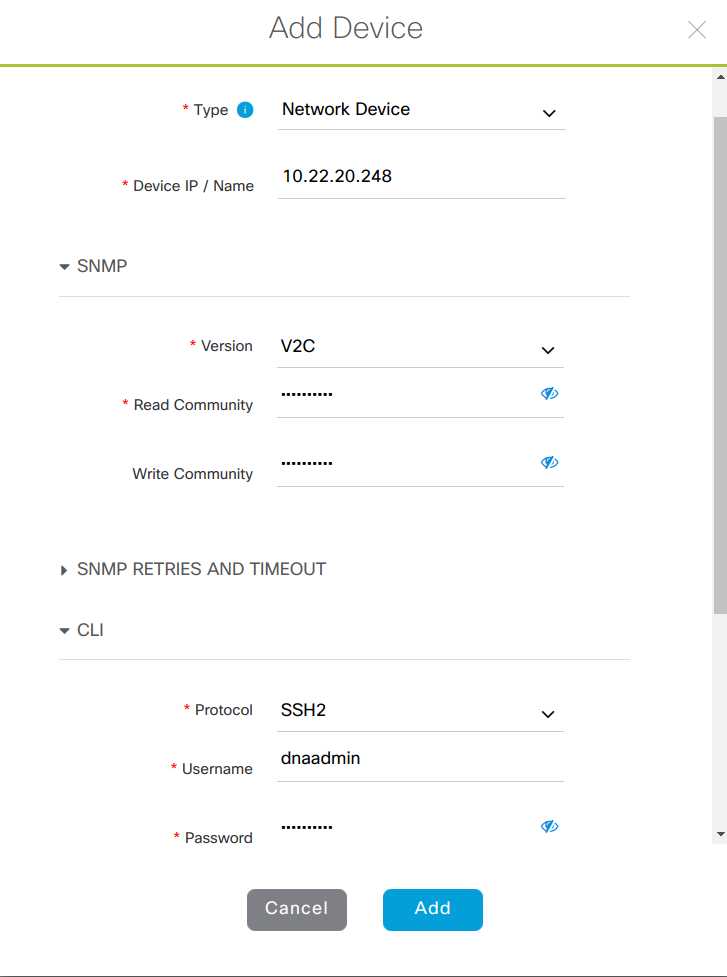
\includegraphics[height=5cm]{img/dna-center-inventory-add-form.png}
	\caption{DNA Center Inventory - Formular Gerät hinzufügen}
	\label{fig:dna-center-inventory-add-form}
\end{figure}

Danach erscheint das Gerät im Inventory. (siehe \ref{fig:dna-center-inventory-index-new})

\begin{figure}[H]
	\centering
	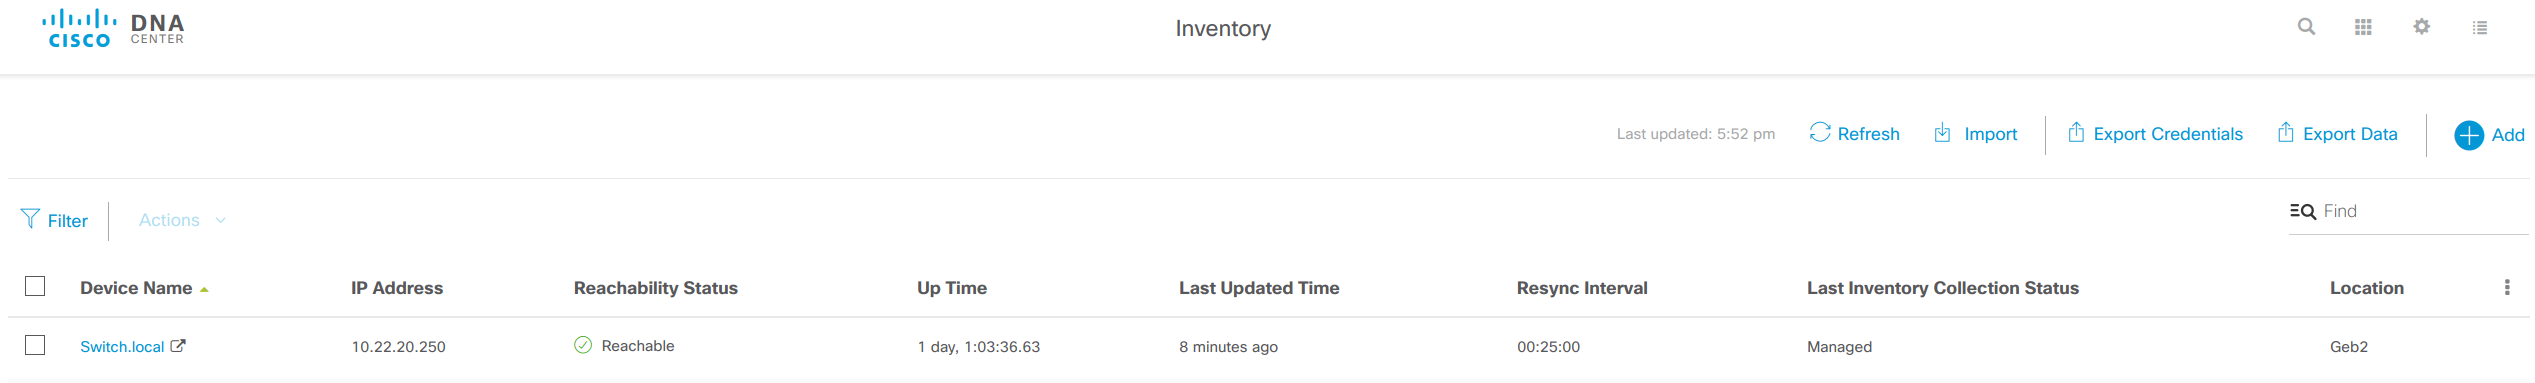
\includegraphics[height=2cm]{img/dna-center-inventory-index-new.png}
	\caption{DNA Center Inventory - Neue Geräte in der Liste}
	\label{fig:dna-center-inventory-index-new}
\end{figure}


\subsection{Image Repository}
Im DNA Center können Netzwerkgeräte automatisch aktualisiert werden. Sobald ein Gerät im Inventory erfolgreich hinzugefügt worden ist, sucht das DNA Center automatisch nach Updates. Allerdings nur, wenn ein CCO Account konfiguriert ist. Die verfügbaren Images sind unter \textit{Desing $\rightarrow$ Global $\rightarrow$ Image Repository} zu finden.

\begin{figure}[H]
	\centering
	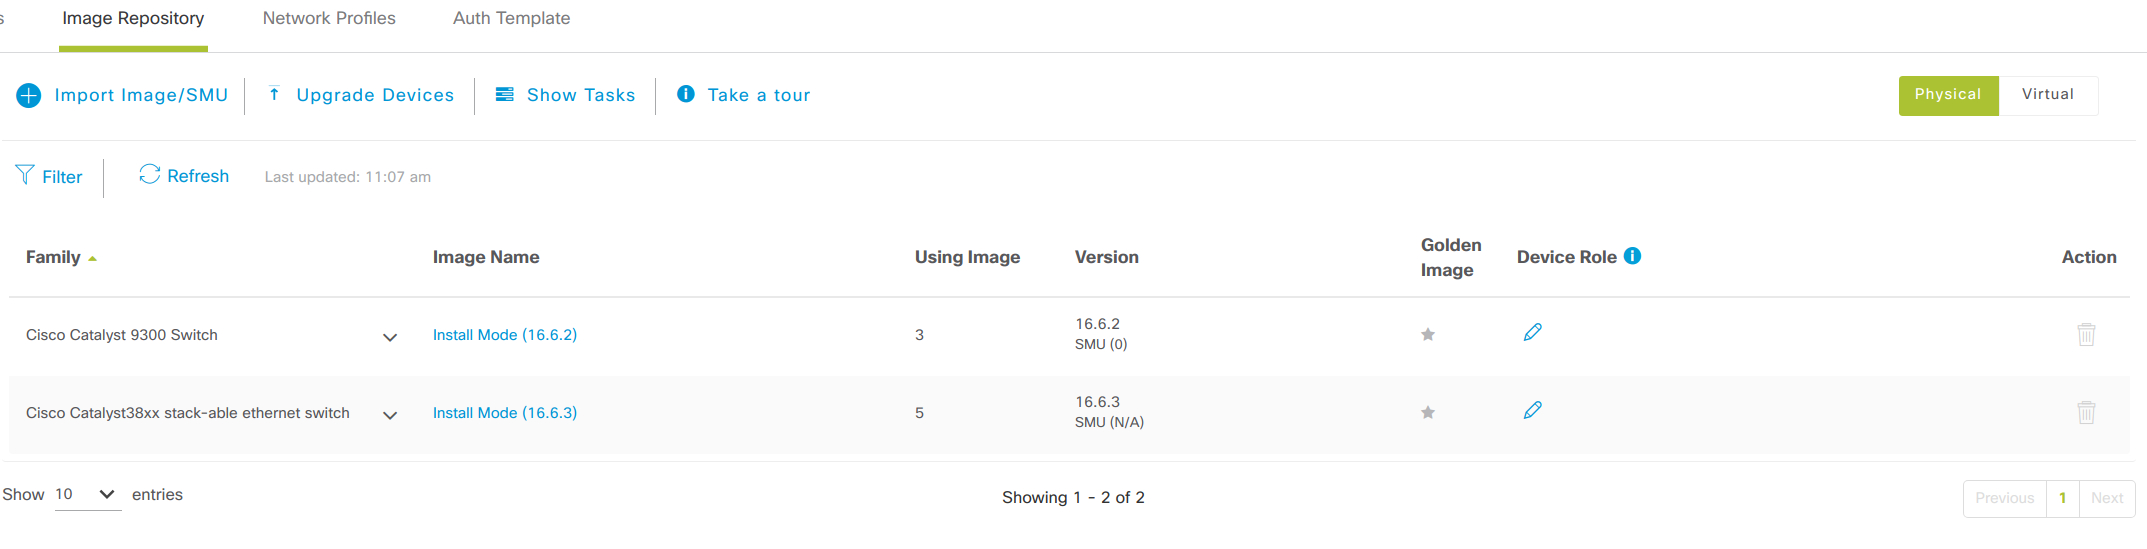
\includegraphics[height=2cm]{img/dna-center-design-image-repository.png}
	\caption{DNA Center Design - Image Respository}
	\label{fig:dna-center-design-image-repository}
\end{figure}

In diesem Image Repository kann das gewünschte Image mit einem "Golden Tag" versehen werden, worauf dieses heruntergeladen wird. 

\subsection{Automatisches Softwareupdate von Netzwerkgeräten}
Die Softwareupdates von Netzwerkgeräten können im DNA Center unter \textit{Provision $\rightarrow$ Devices $\rightarrow$ Inventory} durchgeführt werden. Ebenfalls wird hier angezeigt, welche Softwareversion zur Zeit auf dem Gerät installiert ist und ob diese aktuell ist.

\begin{figure}[H]
	\centering
	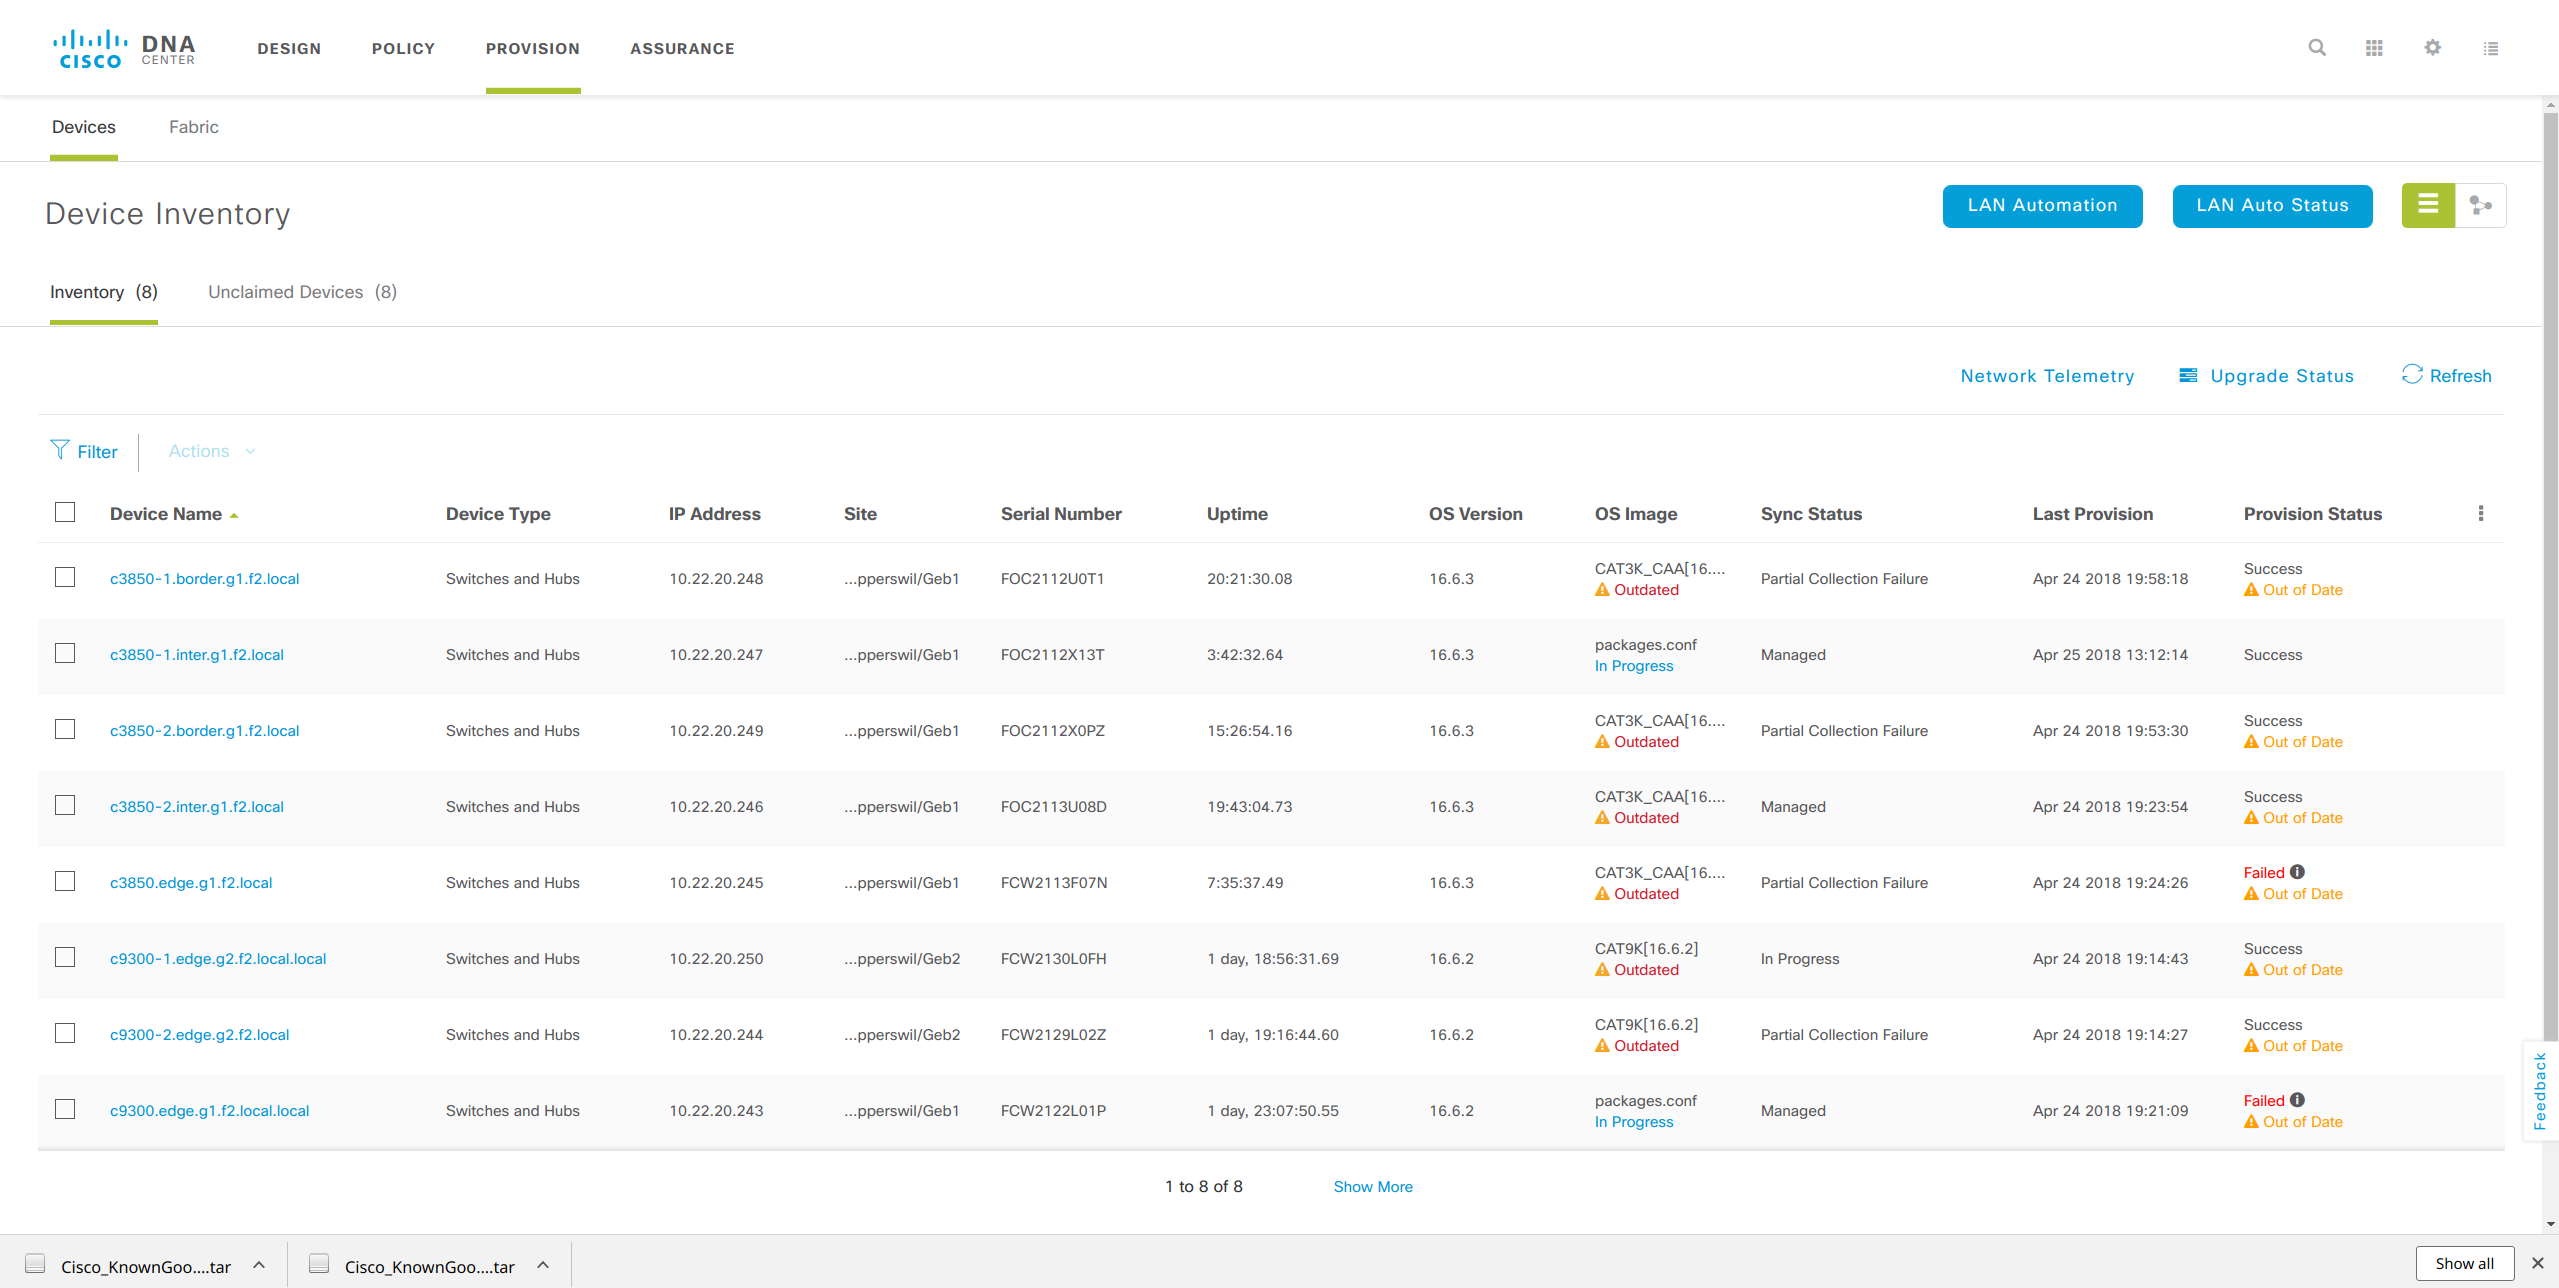
\includegraphics[height=8cm]{img/updates/Selection_070.png}
	\caption{DNA Center Provision - Die OS Versionen sind outdated.}
	\label{fig:dna-center-provision-updates}
\end{figure}

Das automatische Softwareupdate hat bei keinem von unseren Switches oder Routern geklappt. Nachfolgend eine kleine Übersicht über die verschiedenen Update Methoden und ausgeführten Versuche.

\begin{table}[H]
	\rowcolors{2}{gray!25}{white}
	\centering
	\begin{tabular}{ | l | l |}
	\hline
	\rowcolor{gray!50}
	\textbf{Methode} & \textbf{Resultat} \\
	\hline	
	\makecell
	{DNA Center über HTTP und SFTP} & Fehlgeschlagen (siehe \ref{fig:dna-center-provision-updates-1}) \\
	\hline
	CLI - HTTPS    & Fehlgeschlagen (siehe \ref{fig:dna-center-provision-updates-2}) \\
	\hline
	CLI - SCP      & Fehlgeschlagen (siehe \ref{fig:dna-center-provision-updates-3}) \\
	\hline
	CLI - TFTP     & Erfolgreich (siehe \ref{fig:dna-center-provision-updates-4}) \\	
	\hline
	\end{tabular}
	\captionof{table}{Softwareupdate - Übersicht Methoden und ausgeführten Versuche}
\end{table}

Beim Versuch die Softwareupdates im DNA Center über HTTP oder SFTP durchzuführen, wurden folgende Fehlermeldungen angezeigt.

\begin{figure}[H]
	\centering
	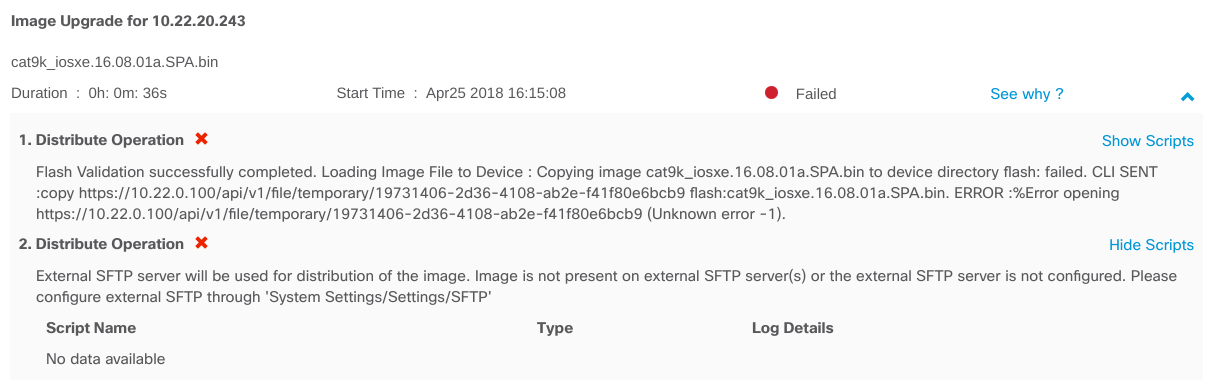
\includegraphics[height=5cm]{img/updates/Selection_071.png}
	\caption{Fehlermeldung Updatevorgang via DNA Center}
	\label{fig:dna-center-provision-updates-1}
\end{figure}

Die Upgrade Prozesse wurden schon beim Kopieren der einzelnen Images nach unterschiedlicher Dauer immer abgebrochen.

\subsection{Manuelles Softwareupdate}
Da wie oben beschrieben das automatische Update nicht funktionierte, wurde in einem nächsten Schritt versucht, die Updates manuell auf die Netzwerkgeräte zu installieren. 

\begin{figure}[H]
	\centering
	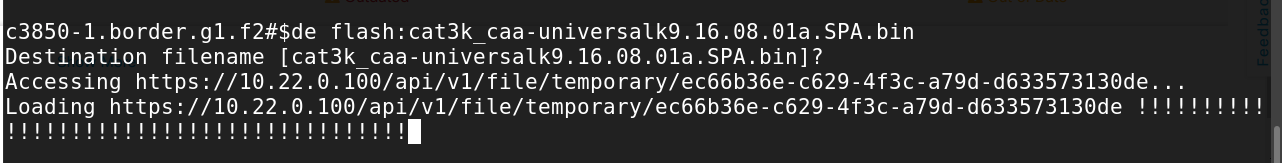
\includegraphics[height=2cm]{img/updates/Selection_082.png}
	\caption{Firmwareupdate Switch via CLI HTTPs}
	\label{fig:dna-center-provision-updates-2}
\end{figure}
Das Kopieren via HTTPS und SCP war sehr unzuverlässig und wurde nach einer gewissen Dauer abgebrochen.

\begin{figure}[H]
	\centering
	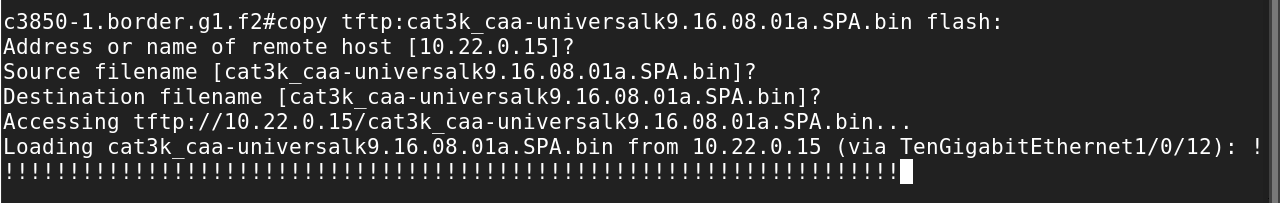
\includegraphics[height=2cm]{img/updates/Selection_111.png}
	\caption{Firmwareupdate Switch via CLI TFTP}
	\label{fig:dna-center-provision-updates-4}
\end{figure}
Mittels TFTP Server konnten die Devices schlussendlich erfolgreich aktualisiert werden.

\subsection{Lizenzen}
Die Lizenzen bezieht das DNA Center vom konfigurierten CCO Account. 
\begin{figure}[H]
	\centering
	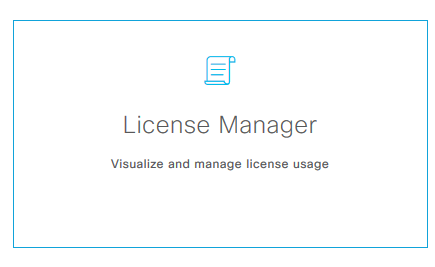
\includegraphics[height=3cm]{img/LicenceManager_001.png}
	\caption{Der Licence Manager ist über das Dashboard erreichbar.}
	\label{fig:dna-center-licence-1}
\end{figure}

\begin{figure}[H]
	\centering
	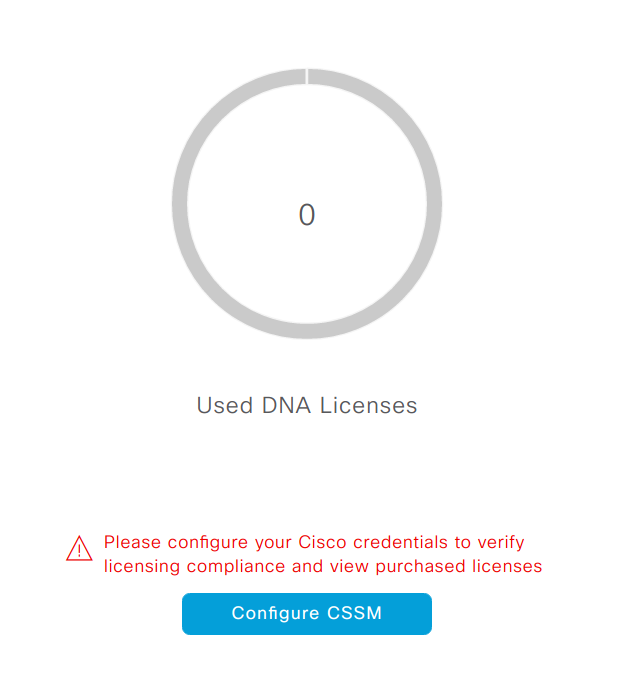
\includegraphics[height=6cm]{img/Selection_006.png}
	\caption{Ohne verlinkten CSSM Account können keine Lizenzen zugewiesen werden.}
	\label{fig:dna-center-licence-3}
\end{figure}

\begin{figure}[H]
	\centering
	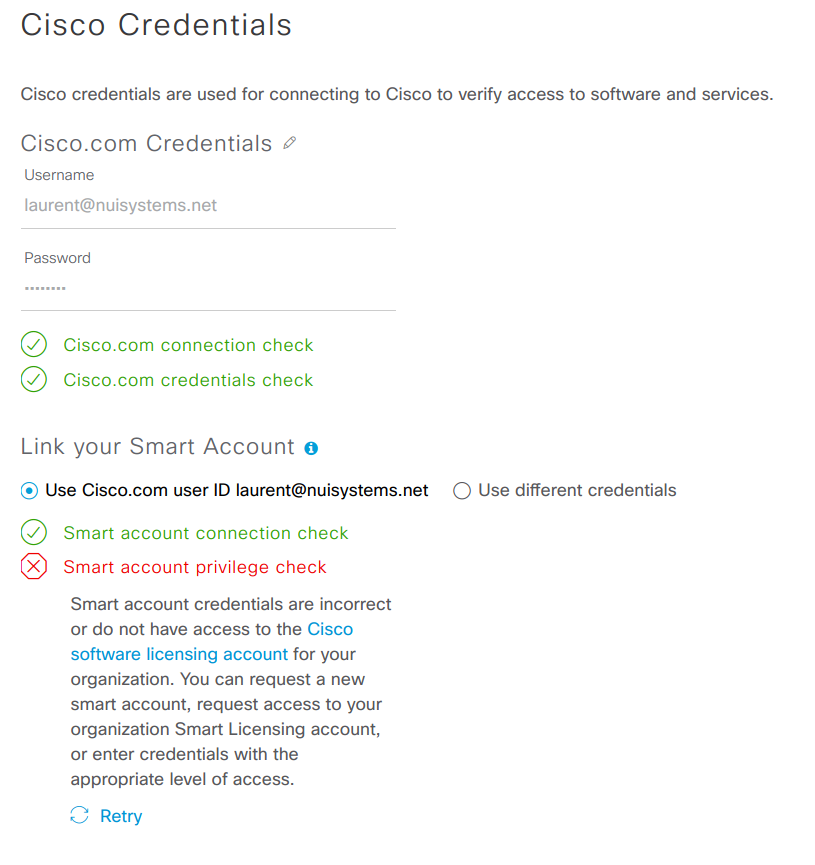
\includegraphics[height=6cm]{img/Selection_008.png}
	\caption{Der im DNA Center hinterlegte Cisco Account muss Zugriff zum entsprechenden Smart Account haben.}
	\label{fig:dna-center-licence-4}
\end{figure}

\begin{figure}[H]
	\centering
	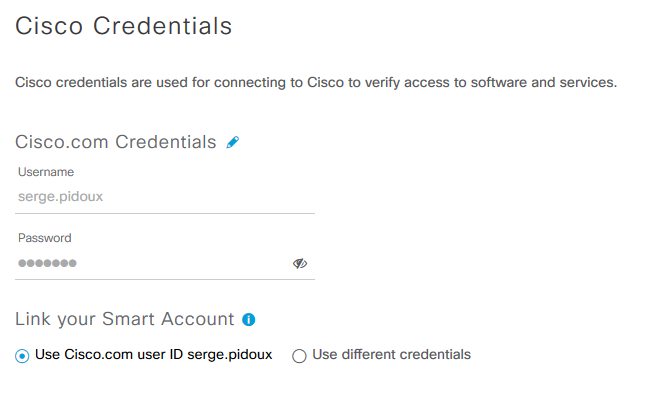
\includegraphics[height=5cm]{img/LicenceManager_002.png}
	\caption{Der korrekt hinterlegte Account}
	\label{fig:dna-center-licence-5}
\end{figure}

\begin{figure}[H]
	\centering
	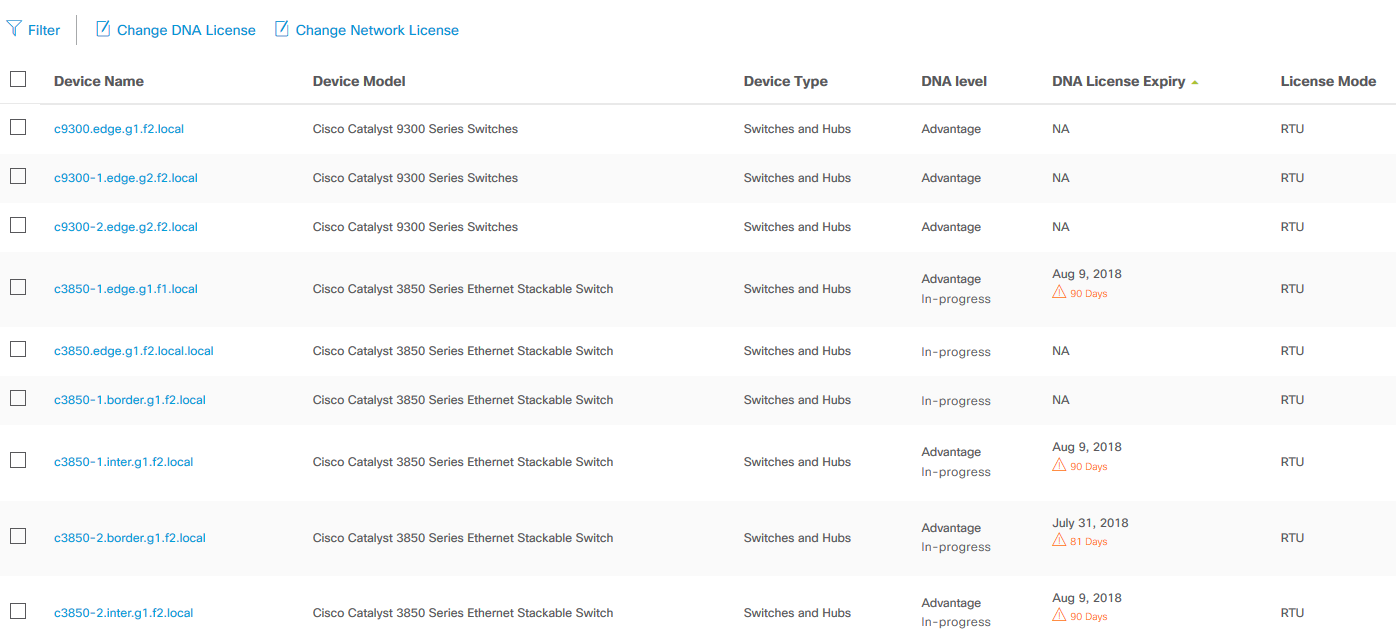
\includegraphics[height=8cm]{img/LicenceManager_003.png}
	\caption{Übersicht über die den Netzwerkkomponenten zugewiesenen Lizenzen}
	\label{fig:dna-center-licence-6}
\end{figure}

\begin{figure}[H]
	\centering
	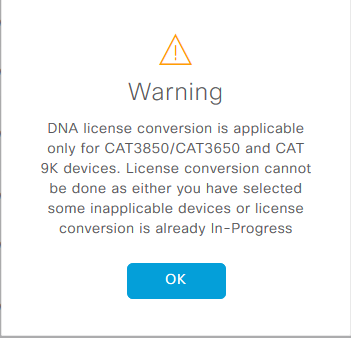
\includegraphics[height=6cm]{img/LicenceManager_004.png}
	\caption{Nicht jedem Gerät kann eine Lizenz zugewiesen werden (Siehe Tabelle)}
	\label{fig:dna-center-licence-7}
\end{figure}

\begin{table}[H]
	\rowcolors{2}{gray!25}{white}
	\centering
		\begin{tabular}{ | c | c | }
		\hline
		\rowcolor{gray!50}
		\textbf{Geräteserie} & 	\textbf{Lizenzzuweisung möglich} \\
		\hline
		Cisco Catalyst 9300 Series Switches & Ja \\
		\hline
		Cisco Catalyst 3850 Series Ethernet Stackable Switch & Ja \\
		\hline
		Cisco 4400 Series Integrated Services Routers & Nein \\
		\hline
	\end{tabular}
	\captionof{table}{Netzwerkgeräte Lizenzzuweisung}
\end{table}

\subsection{Device Provisioning via DNA Center}
\label{device-provisioning}
Um den einzelnen Netzwerkgeräten einen Namen und die Basis Konfiguration zu geben, werden im DNA Center unter \textit{Provision $\rightarrow$ Devices} die zu provisionierenden Geräte ausgewählt. Danach wird \textit{Action $\rightarrow$ Provision Device} der Provision Vorgang gestartet.

Dabei wird die komplette Konfiguration, die das DNA Center für ein Device vorsieht auf dem Gerät konfiguriert. Sind Templates für den entsprechende Devicetyp konfiguriert worden, werden diese ebenfalls angewendet.
Templates können im Template Editor erstellt und entsprechenden Gerätetypen zugewiesen werden.

\begin{figure}[H]
	\centering
	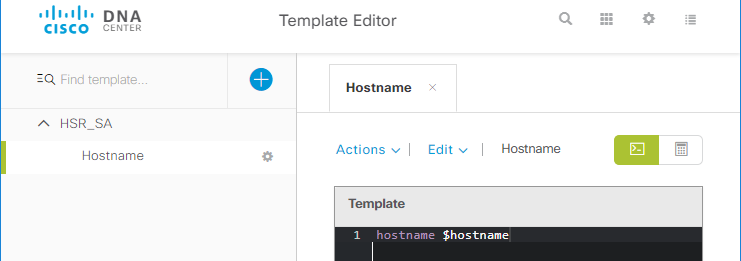
\includegraphics[width=12cm]{img/templateeditor.png}
	\caption{DNA Center - Template Editor}
	\label{fig:Template Editor}
\end{figure}


\subsection{Fabric Konfigurieren}
\label{fabric-configuration}
Nach der manuellen Konfiguration des Underlays, dem hinzufügen der Geräte, dem Update und dem Provisionieren, konnten wir endlich die Fabric konfigurieren. 

Erreichbar ist das unter \textit{Provision $\rightarrow$ Fabric}. Nachfolgend wird die Fabric des entsprechenden Standortes ausgewählt.

Den einzelnen Netzwerkgeräten werden nun mit Rechtsklick folgende Rollen zugeteilt:
\begin{itemize}
	\item Border
	\item Border + CP (Control Plane)
	\item Edge
\end{itemize}

Nachdem alle Geräte der entsprechenden Fabric zugeteilt worden sind, kann die Konfiguration gespeichert werden und wird auf die Geräte geschrieben. 

\begin{figure}[H]
	\centering
	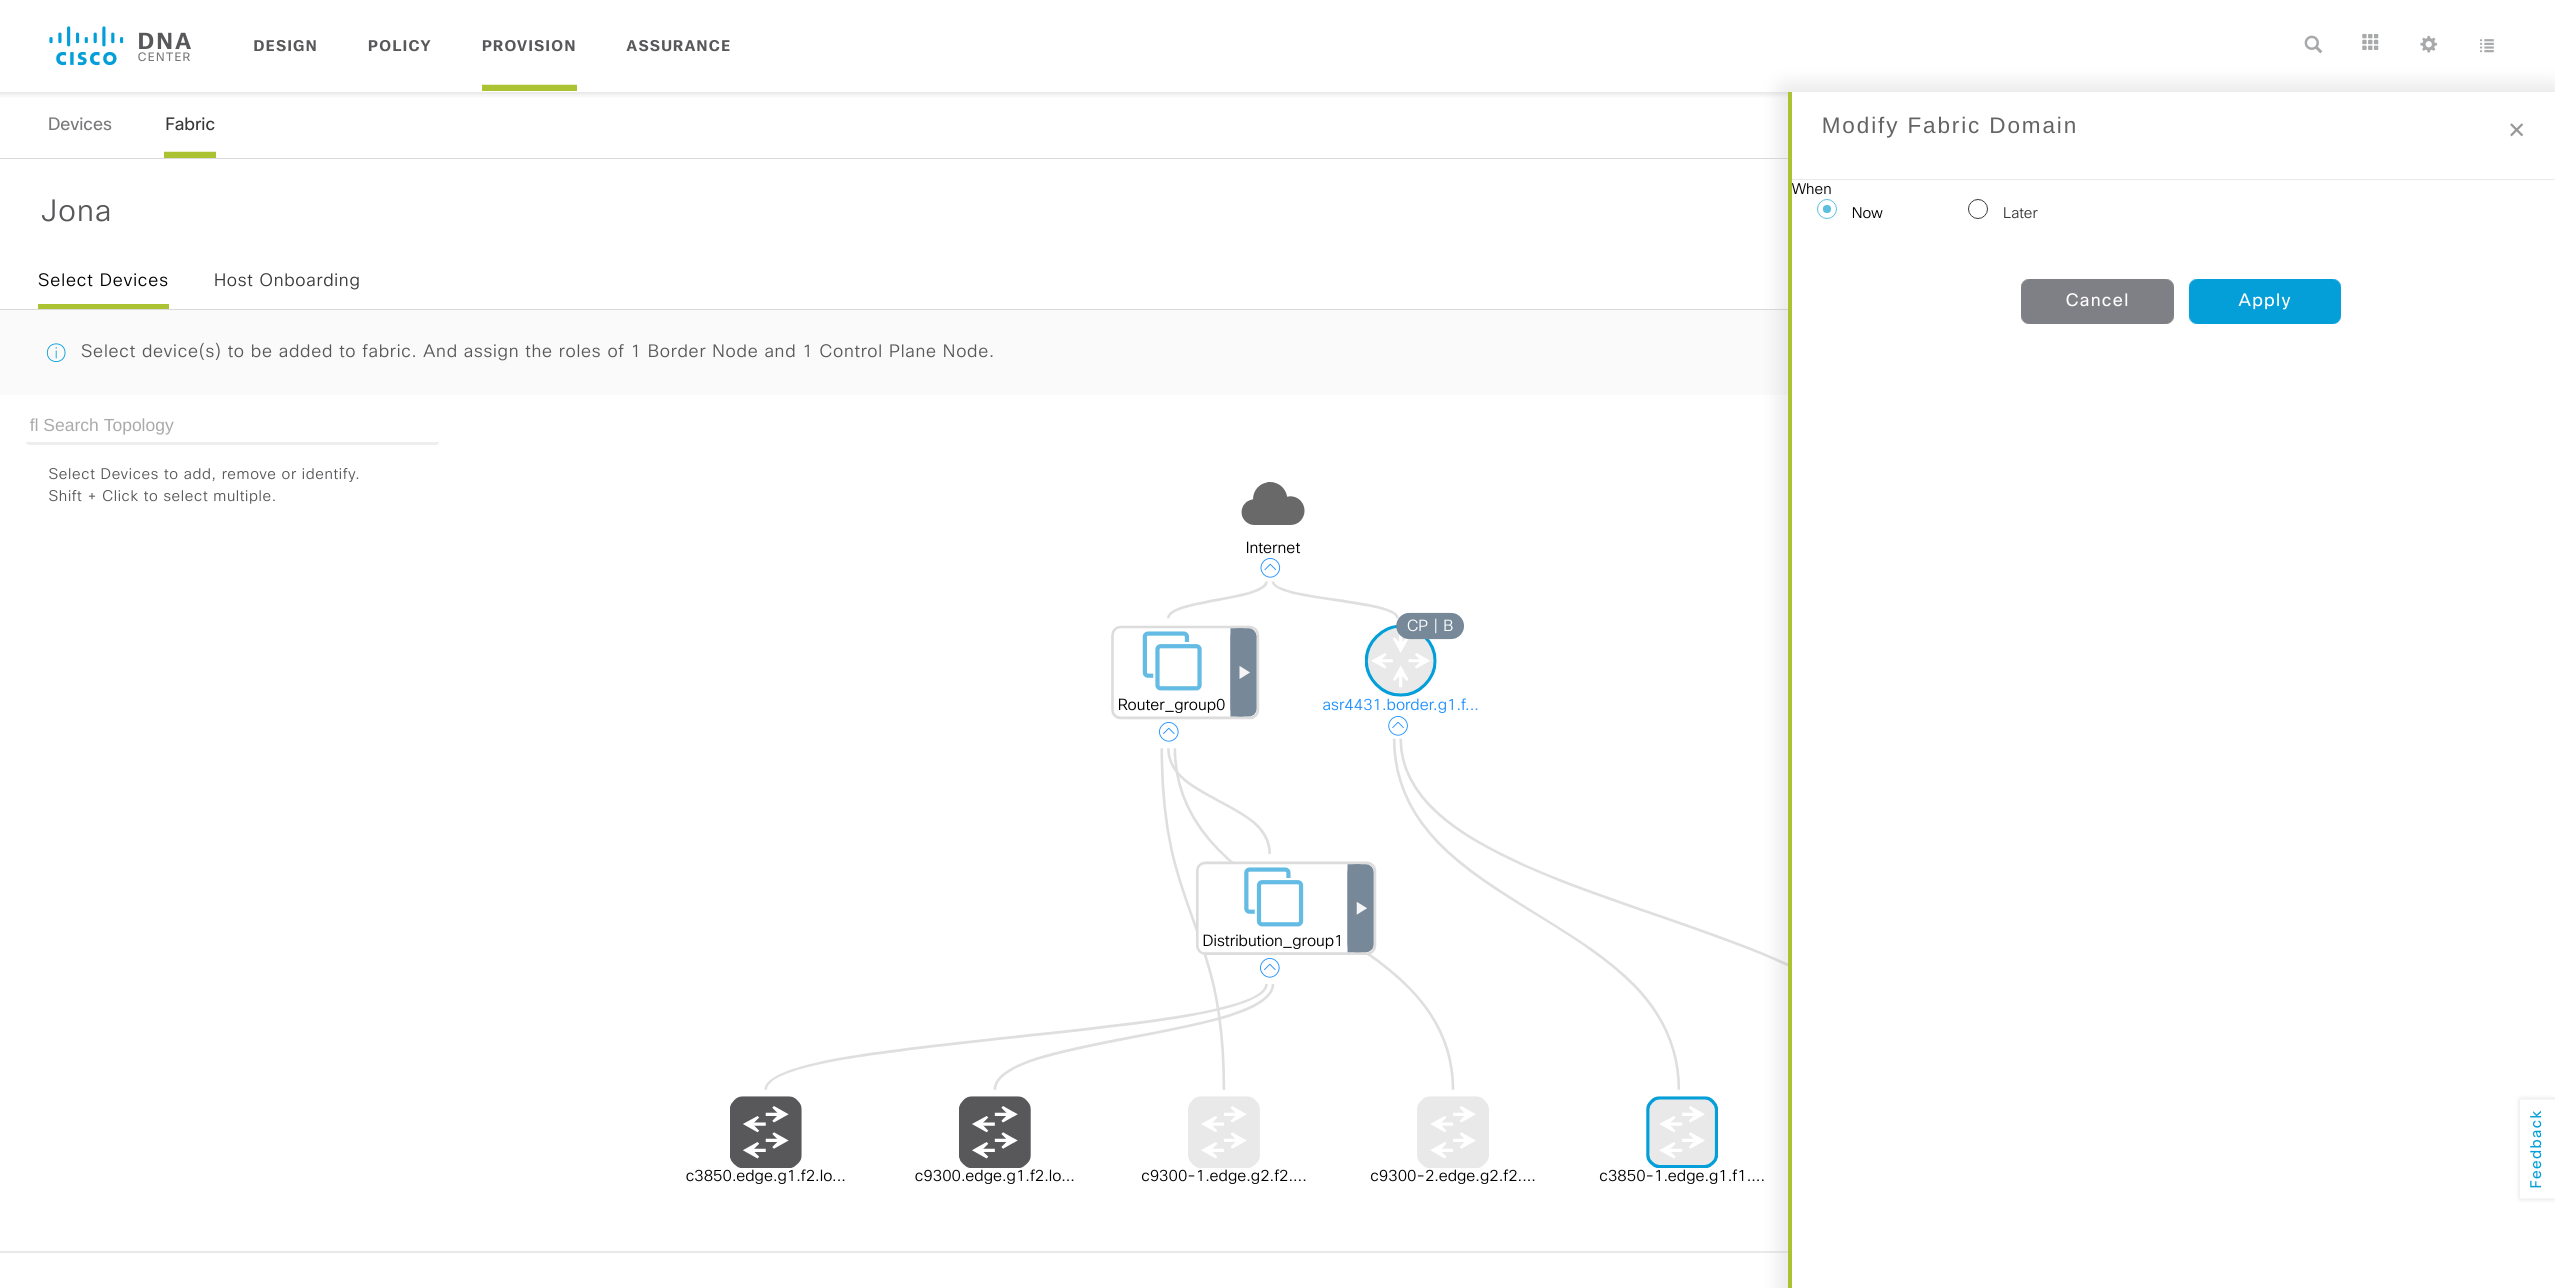
\includegraphics[width=16cm]{img/dna-center-fabric-1.png}
	\caption{DNA Center Provision - Fabric - Nach der Zuteilung wird die Konfiguration auf die Geräte geschrieben.}
	\label{fig:IP Base and Services}
\end{figure}

\begin{table}[H]
	\rowcolors{2}{gray!25}{white}
	\centering
	\begin{tabular}{| l | l | l | l | l |}
		\hline
		\rowcolor{gray!50}
		\textbf{Darstellung} & \makecell{\textbf{Teil einer}\\ \textbf{Fabric}} & \makecell{\textbf{Änderung}\\ \textbf{ausstehend}} & \textbf{Provisioniert} & \textbf{Bemerkung} \\
		\hline
		Dunkelgrau & Ja & Nein & Nein & fremde Fabric \\
		\hline
		Hellgrau & Nein & Nein & Nein &  \\
		\hline
		Grau mit blauem Rand & Ja & Ja & Nein & nicht deployed\\
		\hline
		Blau & Ja & Nein & Ja & aktuelle Fabric\\
		\hline
		Umrandung mit Pfeil & - & - & - & Gruppierte Geräte\\	
		\hline
	\end{tabular}
	\captionof{table}{DNA Center Provision - Fabric - Darstellung}
\end{table}

\subsection{DNA Center Reset}
Da das Overlay Provisioning auch nach mehreren Versuchen nur teilweise funktioniert hatte, haben wir entschlossen, die Switches zusätzlich über das Out-of-Band Management zu verbinden, da dies in mehreren Videos von Cisco so erwähnt wird und im ersten Release zwingend nötig war. \\
Dazu benötigt das DNA Center ein zusätzliches Interface im Out-of-Band Management Netz. Um dieses einzurichten, muss der initiale Wizard erneut gestartet werden. 

\begin{lstlisting}[language=bash]
$ maglev-config-wizard #DO NOT EXECUTE THIS COMMAND
\end{lstlisting}

Als Folge dieses Befehls, nachdem alle Parameter eingegeben wurden, kam die folgende Meldung:

\begin{figure}[H]
	\centering
	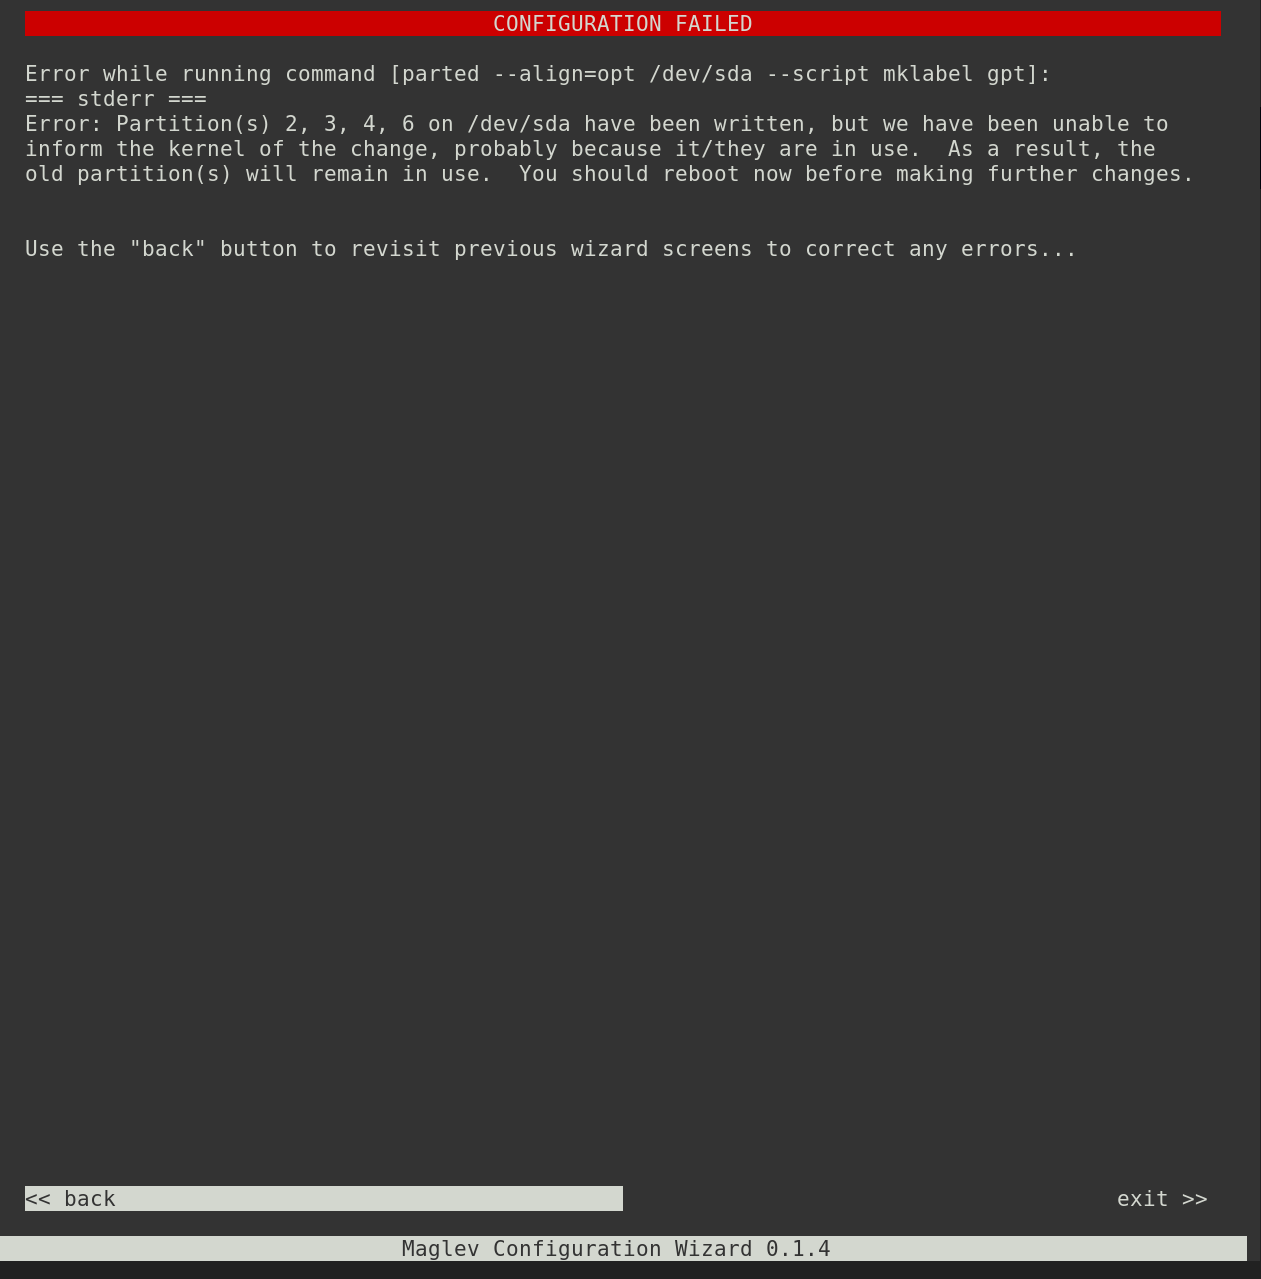
\includegraphics[height=10cm]{img/dna-center-reset-fail-1.png}
	\caption{DNA Center - maglev-config-wizard - Fehlermeldung}
	\label{fig:dna-center-reset-1}
\end{figure}

Nach einem Neustart der Appliance erschien die folgende Meldung und das System bootete nicht mehr. 
\begin{figure}[H]
	\centering
	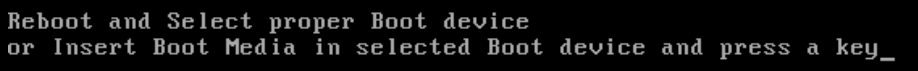
\includegraphics[height=1cm]{img/dna-center-reset-fail-2.png}
	\caption{DNA Center - Boot Fehlermeldung}
	\label{fig:dna-center-reset-2}
\end{figure}

Es stellte sich heraus, dass wir den falschen Wizard gestartet hatten.
Korrekt wäre der folgende Befehl gewesen:

\begin{lstlisting}[language=bash]
$ sudo maglev-config update
\end{lstlisting}

Allerdings hätte auch der erste Befehl nicht dazu führen sollen, dass das System nicht mehr startet.

\paragraph{Neuinstallation} 
~\\
In der Folge war es nötig, dass DNA Center komplett neu zu installieren. Dazu ist ein entsprechendes ISO nötig, welches leider nicht mitgeliefert wird. Dieses kann bei Cisco via TAC Case angefordert werden. Mit dem ISO muss dann ein bootbarer USB Stick erstellt werden.

\begin{figure}[H]
	\centering
	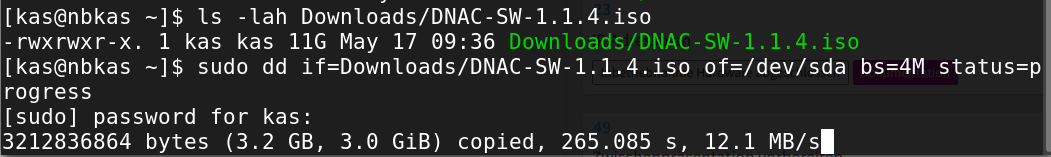
\includegraphics[height=2cm]{img/dna-center-reset-iso.png}
	\caption{DNA Center - Neuinstallation - Installations ISO wird auf USB Drive kopiert}
	\label{fig:dna-center-iso-1}
\end{figure}

Anschliessend kann der USB-Stick in die Appliance gesteckt und diese gestartet werden. Die initiale Installation ist in Abschnitt \ref{DNACenterSetup_Installation} gezeigt. 

\alertwarningbox{
	Nach der Neuinstallation sind alle Daten und die Konfiguration gelöscht. Eine Option die Konfiguration beizubehalten gibt es nicht.
}

\section{Vorgehen Versuch 2}
\begin{figure}[H]
	\centering
	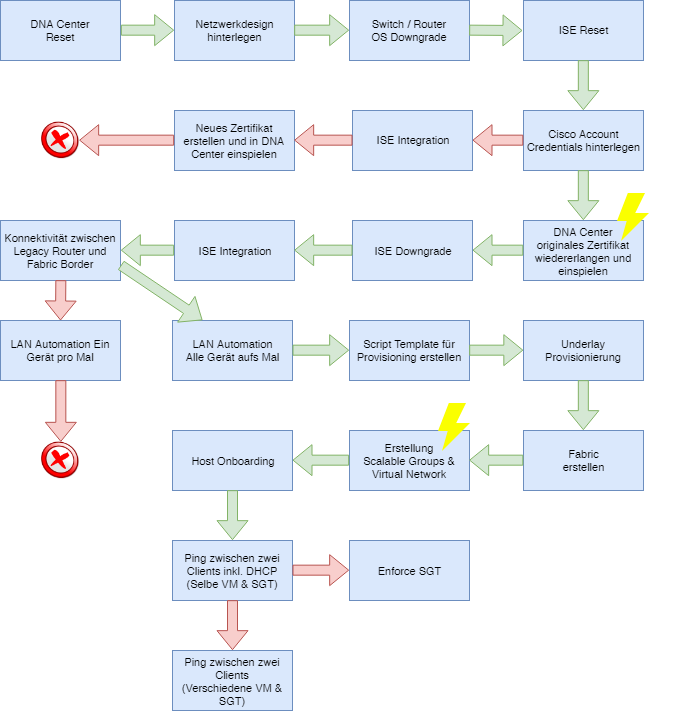
\includegraphics[height=14cm]{img/vorgehen2.png}
	\caption{Grafische Übersicht über das Vorgehen beim zweiten Versuch}
	\label{fig:vorgehen-2}
\end{figure} 

\subsection{Vorarbeiten}

Damit im zweiten Versuch keine Probleme mit bestehenden Konfigurationen entstehen, haben wir den alle Konfigurationen in Infoblox gelöscht und ISE auf den Werkszustand zurückgesetzt. \\
Des Weiteren wurde auf allen Netzwerkdevices die IOS-XE Version 16.6.3 installiert, da gemäss Patrick Mosimann von Cisco nur diese Version mit dem aktuellen DNA Center kompatibel ist.

\subsubsection{ISE reset}
Um die Störungen durch alte Konfigurationen zu vermeiden, wurde das Cisco ISE Center ebenfalls zurückgesetzt. Dies kann einfach mittels eines Befehls durchgeführt werden.

\begin{lstlisting}[language=bash]
ISE/admin# applicaiton reset-config ise
\end{lstlisting}

\begin{figure}[H]
	\centering
	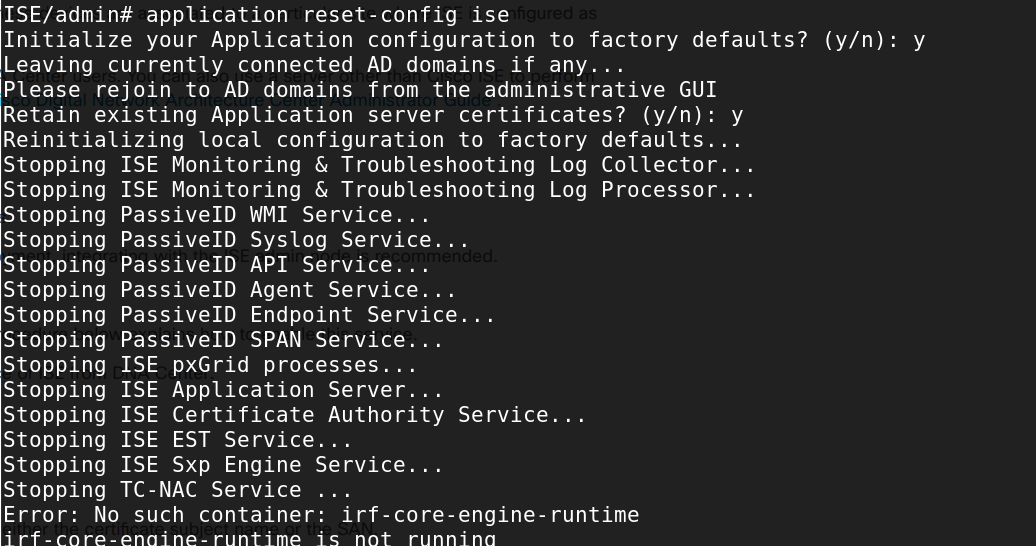
\includegraphics[height=6cm]{img/secondtry/s2t-cisco-ise-reset.png}
	\caption{Cisco ISE Reset}
	\label{fig:dna-ise-reset-1}
\end{figure}


\subsection{DNA Center Update}

Wie im ersten Versuch, haben wir das DNA Center nach der Installation auf den aktuellsten Stand geupdated. Dieser Vorgang wurde im Abschnitt \ref{DNACenter_Updates} gezeigt. Dies war mittlerweile die Version 1.1.6. Im ersten Versuch arbeiteten wir mit den Versionen 1.1.4 und 1.1.5.

\subsection{DNA Center Netzwerk Design}
Das Netzwerkdesign wurde analog unserem ersten Versuch in Abschnitt \ref{DNACenterNetwork_Design} erstellt.


\subsection{ISE Integration}
Bei der Integration des ISE wollten wir gleich vorgehen, wie im ersten Versuch. Es stellt sich aber heraus, dass im Release 1.1.6 in Kombination mit ISE 2.4 geprüft wird, ob das DNA Center über ein Zertifikat verfügt, das den Hostname oder die IP des DNA Centers im Common Name hat. Aus diesem Grund haben wir das Zertifikat des DNA Centers durch eines ersetzt, dass diese Bedingung erfüllt.

\begin{figure}[H]
	\centering
	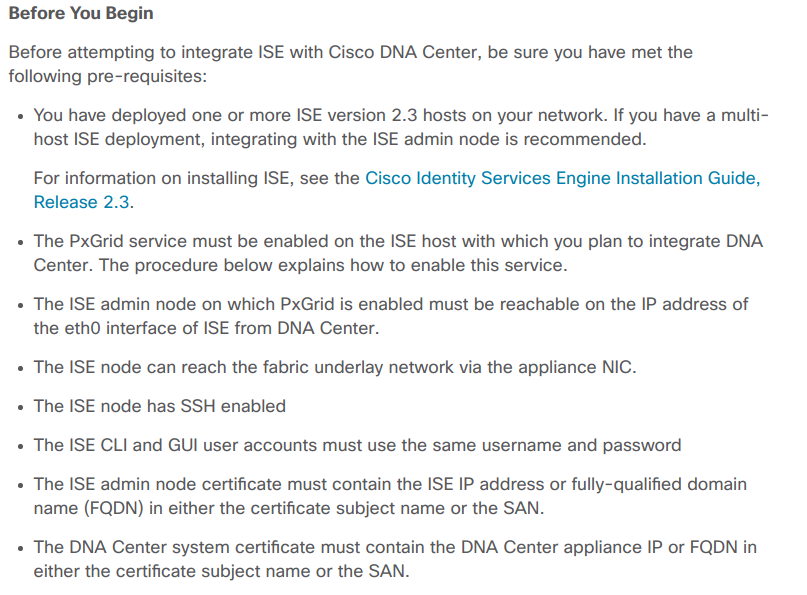
\includegraphics[height=6cm]{img/secondtry/ise-prerequirements.png}
	\caption{ISE Integration Prerequirements}
	\label{fig:dna-ise-prerequirements}
	\cite{cisco-dna-installation-guide}
\end{figure}

Das Zertifikat kann unter \textit{Settings $\rightarrow$ Settings $\rightarrow$ Certificate $\rightarrow$ Replace Certificate} ausgetauscht werden. Es ist möglich Zertifikate im PEM Format oder als PKCS Datei hochzuladen. 

\begin{figure}[H]
	\centering
	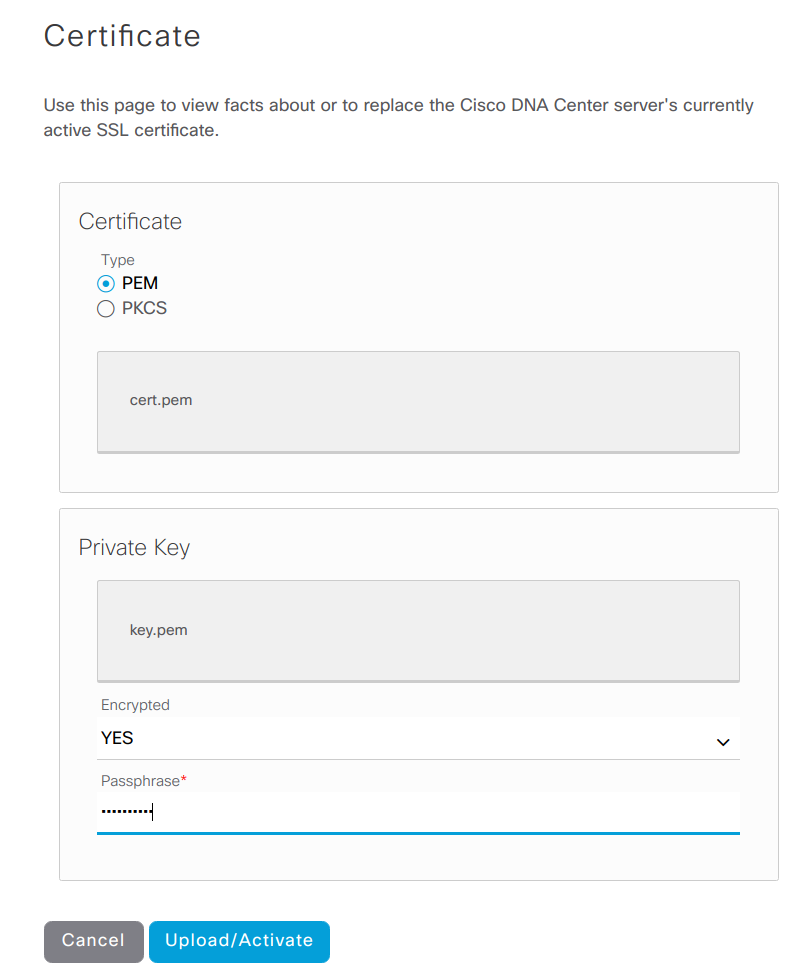
\includegraphics[height=8cm]{img/secondtry/dna-center-certificate-replacement.png}
	\caption{DNA Center Certificate Replacement}
	\label{fig:dna-certificate-replacement}
\end{figure}

Nachdem das Zertifikat durch ein self-signed Zertifikat ausgetauscht wurde, welches die Bedingung erfüllt, dass die IP oder der Hostname im Common Name sein muss, funktionierte die ISE Integration ohne weitere Probleme.

\subsection{LAN Automation}

Bevor die LAN Automation gestartet werden kann, müssen folgende Bedinungen für das Seed Device erfüllt sein:
\begin{itemize}
	\item Aktives SSH
	\item IP Konnektivität
\end{itemize}

\subsubsection{Verbindung zwischen Legacy Router und Border Switch}
Damit die LAN Automation gestartet werden kann, muss zuerst ein Seed Device eingerichtet werden, dass vom DNA Center aus erreichbar ist. Dies kann mit untenstehenden Befehlen über ein temporäres VLAN erreicht werden. 

\paragraph{Konfiguration auf Border Switch}
\begin{lstlisting}[language=bash]
# interface lo0
#   ip address 10.22.30.1 255.255.255.255
#
# interface Te1/0/12
#   switchport trunk native vlan 100
#   switchport mode trunk
#
# interface vlan 100
#   ip adress 10.22.31.1 255.255.255.252
# 
# ip route 10.22.0.0 255.255.255.0 10.22.31.2
\end{lstlisting}

\paragraph{Konfiguration auf Legacy Router}
\begin{lstlisting}[language=bash]
# interface GigabitEthernet0/0/1.100
#   encapsulation dot1Q 100
#   ip address 10.22.31.2 255.255.255.252
#
# ip route 10.22.30.1 255.255.255.255 10.22.31.1
\end{lstlisting}

\subsubsection{Discovery}
Da der oben konfigurierte Border Router als Seed Device genutzt werden soll um die restlichen Geräte zu finden und zu deployen, muss dieses im DNA Center bekannt gemacht werden. Am einfachsten geht dies über die Discovery Funktion. Diese kann mittels \textit{Discovery $\rightarrow$ New Discovery} eingerichtet werden. Die Discovery kann gemäss untenstehender Grafik konfiguriert werden.

\begin{figure}[H]
	\centering
	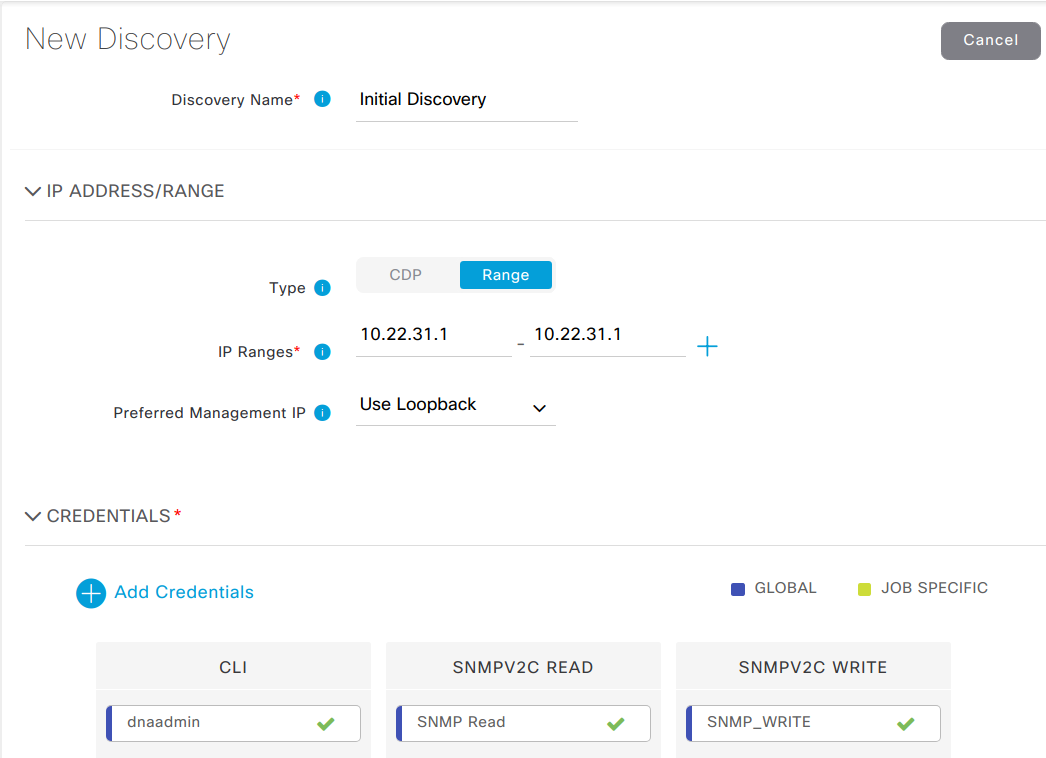
\includegraphics[height=8cm]{img/secondtry/dna-discovery.png}
	\caption{DNA Center Discovery}
	\label{fig:dna-discovery}
\end{figure}

Sobald das Device gefunden wurde, erscheint dieses im Inventory. Damit dieses als Seed Device verwendet werden kann, ist zuerst ein Provisioning wie in \ref{device-provisioning} beschrieben nötig und das Device muss einer Fabric hinzugefügt werden \ref{fabric-configuration}. 

Beim Provisioning ist aber aufgefallen, dass es Probleme mit der Verbindung zwischen dem Border Switch und dem ISE gibt. Patrick Mosimann hat uns dann erklärt, dass das DNA Center in den aktuell verfügbaren Versionen ausschliesslich mit ISE in der Version 2.3 kompatibel ist.\\
Unglücklicherweise war in unserer Lab Umgebung die Version 2.4 installiert. Ein Downgrade ist leider nicht möglich, weshalb die virtuelle Maschine ausgetauscht werden musste und der ISE erneut ins DNA Center integriert werden musste. 

\subsubsection{LAN Automation PnP}

Nun konnte die eigentliche LAN Automation gestartet werden. Dabei wird, wie in untenstehender Grafik gezeigt ein Seed Device ausgewählt und definiert, auf welchen Interfaces DHCP Requests der anderen Devices beantwortet werden. Zudem muss ein IP Pool angegeben werden, der für folgende Zwecke verwendet wird:
\begin{itemize}
	\item DHCP Pool während dem PnP Vorgang
	\item Loopback Interfaces der Devices
	\item Netze für Point to Point Links
\end{itemize}

Dabei ist zu beachten, dass die Unterteilung des IP Pools nicht optimal ist. Unabhänig von der Grösse des Pools werden beispielsweise nur 30 Adressen für den DHCP Pool reserviert, was in einer grossen Umgebung ein Problem darstellen könnte.

\begin{figure}[H]
	\centering
	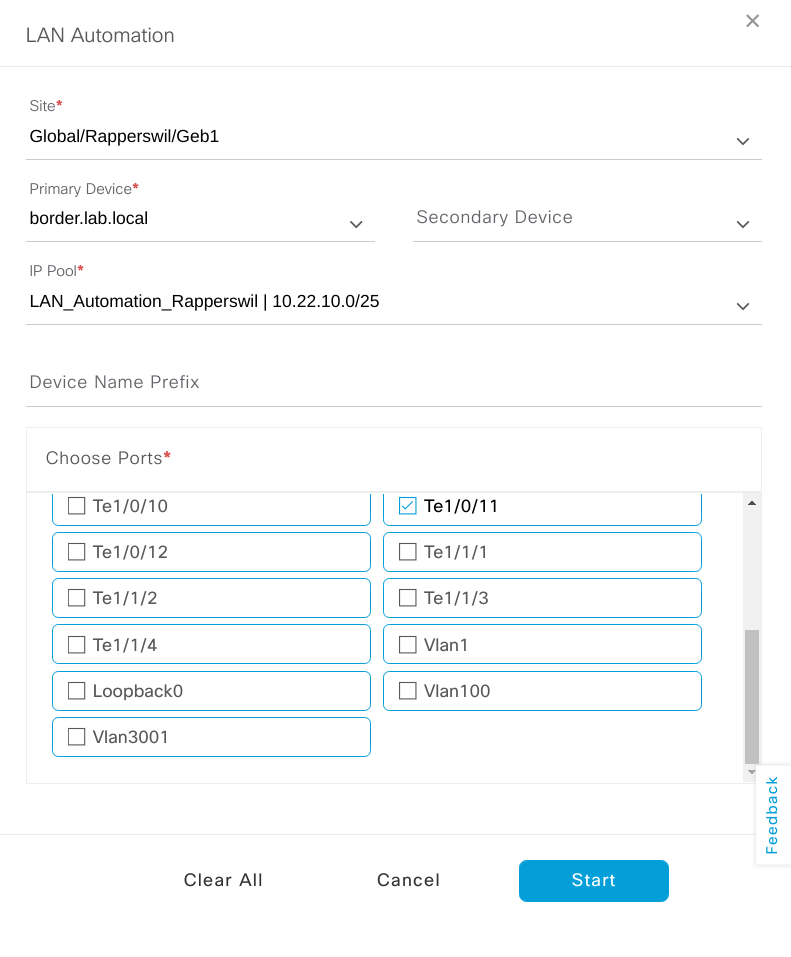
\includegraphics[height=7cm]{img/secondtry/dna-lan-automation-dialog.png}
	\caption{DNA Center - LAN Automation}
	\label{fig:dna-lan-automation-dialog}
\end{figure}

Wir haben dann die LAN Automation gestartet. Dies konfiguriert auf dem Seed Device einen DHCP Server. Werden nun die Konfiguration auf anderen Netzwerkgeräten gelöscht und diese neu gestartet, senden diese DHCP Request, die vom Seed Device beantwortet werden. Die Antworten verweisen auf das DNA Center als PnP Server.
Die Geräte senden nur DHCP Requests, wenn Sie im Zustand sind, der auf untenstehendem Bild ersichtlich ist.

\begin{figure}[H]
	\centering
	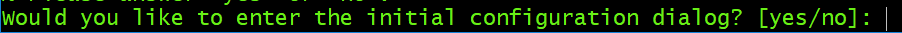
\includegraphics[height=0.5cm]{img/secondtry/cisco-switch-initial-config.png}
	\caption{Cisco Switch - Initial Config - Versucht DHCP und PnP zu machen, solange der Dialog aktiv ist.}
	\label{fig:cisco-switch-initial-config}
\end{figure}

Während des PnP Prozesses wird das Zertifikat, sowie die CA (Certificate Authority) des DNA Centers auf die Netzwerkgeräte kopiert. Dies ist nötig, damit die Verbindung auf HTTPS umgestellt werden kann. Nach diesem Schritt blieb der Setup Prozess jeweils mit folgender Meldung stehen:

\begin{figure}[H]
	\centering
	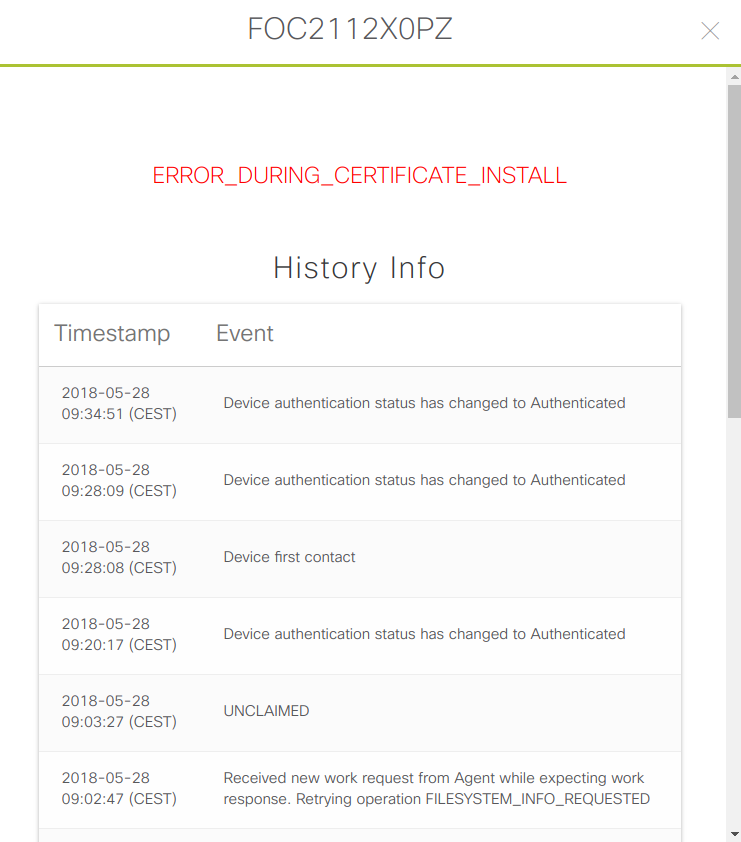
\includegraphics[height=7cm]{img/secondtry/dna-pnp-cert-error.png}
	\caption{LAN Automation - PnP Error}
	\label{fig:dna-pnp-cert-error}
\end{figure}

Es stellte sich heraus, dass das Problem war, dass unser self-signed Zertifikat nicht von der DNA Center CA signiert war und die Netzwerkgeräte daher nicht validiern konnten ob dieses gültig ist. Leider konnte uns auch Patrick Mosimann von Cisco nicht sagen, wie wir dieses Zertifikat signieren können, das ursprüngliche Zertifikat wiederherstellen können oder das Problem anderweitig lösen können. Gemäss dem Installation Guide von Cisco \cite{cisco-dna-installation-guide} kann hier auch ein Zertifikat verwendet werden, dass von einer "Well-Known Certificate Authority" signiert ist. Aus diesem Grund haben wir das Zertifikat auch durch ein korrekt von Lets Encrypt signiertes Zertifikat ausgetauscht. Patrick konnte uns aber nicht sagen, ob diese Authority auf dem Gerät bekannt ist. Auch das korrekt signierte Zertifikat wurde nicht akzeptiert und der PnP Prozess konnte nicht weitergeführt werden. \\
Aus diesem Grund haben wir uns via SSH auf die Appliance eingelogged und dort nach dem ursprünglichen Zertifikat oder der CA gesucht. Nach einer Weile wurden wir fündig und fanden das alte Zertifikat und die CA:\\

\begin{lstlisting}[language=bash]
# $ sudo ls -lah /etc/maglev/.pki/
# [sudo] password for maglev: 
# total 140K
# drwxr-xr-x 2 root 4.0K May 21 06:20 .
# drwxr-xr-x 4 root 4.0K May 21 06:20 ..
# -rw-r--r-- 1 root 1.3K May 17 09:09 apiserver.crt
# -rw------- 1 root 1.7K May 17 09:09 apiserver.key
# -rw-r--r-- 1 root 1.2K May 17 09:09 apiserver-kubelet-client.crt
# -rw------- 1 root 1.7K May 17 09:09 apiserver-kubelet-client.key
# -r--r--r-- 1 root 1.1K May 17 08:49 ca.crt
# -rw-r--r-- 1 root 1.7K May 17 08:49 ca.key
# lrwxrwxrwx 1 root   23 May 17 08:49 ca-key.pem -> /etc/maglev/.pki/ca.crt
# lrwxrwxrwx 1 root   23 May 17 09:09 ca.pem -> /etc/maglev/.pki/ca.crt
# -r-------- 1 root 1.7K May 17 08:49 credentialmanager-key.pem
# -r-------- 1 root  307 May 21 06:20 credentialmanager-openssl.cnf
# -r--r--r-- 1 root 1.1K May 17 08:49 credentialmanager.pem
# -r-------- 1 root 1.7K May 17 08:49 encryptionmanager-key.pem
# -r-------- 1 root  307 May 21 06:20 encryptionmanager-openssl.cnf
# -r--r--r-- 1 root 1.1K May 17 08:49 encryptionmanager.pem
# -r-------- 1 root 1.7K May 17 08:49 encryption_seed-key.pem
# -r--r--r-- 1 root  981 May 17 08:49 encryption_seed.pem
# -rw-r--r-- 1 root 1.1K May 17 09:09 front-proxy-ca.crt
# -rw------- 1 root 1.7K May 17 09:09 front-proxy-ca.key
# -rw-r--r-- 1 root 1.1K May 17 09:09 front-proxy-client.crt
# -rw------- 1 root 1.7K May 17 09:09 front-proxy-client.key
# -r-------- 1 root 1.7K May 17 08:49 kong-key.pem
# -r-------- 1 root  299 May 21 06:20 kong-openssl.cnf
# -r--r--r-- 1 root 1.1K May 17 08:49 kong.pem
# -r-------- 1 root 1.7K May 17 08:49 kube-admin-key.pem
# -r--r--r-- 1 root  977 May 17 08:49 kube-admin.pem
# -r-------- 1 root 1.7K May 17 08:49 kube-worker-1-key.pem
# -r-------- 1 root  336 May 21 06:20 kube-worker-1-openssl.cnf
# -r--r--r-- 1 root 1.1K May 17 08:49 kube-worker-1.pem
# -r-------- 1 root 1.7K May 17 08:49 maglev-registry-key.pem
# -r-------- 1 root  472 May 21 06:20 maglev-registry-openssl.cnf
# -r--r--r-- 1 root 1.3K May 17 08:49 maglev-registry.pem
# -r-------- 1 root   36 May 17 08:49 passphrase.txt
# -rw-r--r-- 1 root 1.1K May 21 06:20 registry-ca.pem
# -rw------- 1 root 1.7K May 17 09:09 sa.key
# -rw------- 1 root  451 May 17 09:09 sa.pub
\end{lstlisting}

So konnten wir das alte Zertifikat wiederherstellen (sh. \ref{fig:dna-certificate-replacement} ). Dies war kein Problem, da mit ISE Version 2.3 der Hostname und die IP nicht im Common Name sein müssen. Es wäre aber auch möglich gewesen, mit der CA ein neues zu signieren, da die Passphrase für den Private Key der CA in einem Textfile abgelegt ist.\\

Durch das erneute des Zertifikats wurde leider die Trust Verbindung zum ISE gebrochen, weshalb der ISE erneut ins DNA Center integriert werden musste. 

Nun konnten wir die LAN Automation starten und der PnP Prozess auf den Netzwerkgeräten schien zu funktionieren. 

Wir haben dann, wie von Patrick Mosimann vorgeschlagen, die ersten zwei Devices am Standort Rapperswil mit der LAN Automation konfiguriert, was einwandfrei funktioniert hat. Damit die Konfiguration auf die Geräte geschrieben wird, muss die LAN Automation beendet werden. Anschliessend wiederholten wir diesen Vorgang für die nächsten zwei Geräte. Dabei stellte sich heraus, dass die generierte Konfiguration unbrauchbar ist, da nur einzelne Point to Point Links konfiguriert wurden, aber nicht alle die nötig gewesen wären. \\
Da es sich bei der LAN Automation um ein Basisfeature handelt, wollten wir die Underlay Konfiguration nicht manuell erstellen und versuchten die Ursache für diesen Fehler zu finden. Schlussendlich hat uns folgendes Vorgehen zum Erfolg geführt:
\begin{itemize}
	\item LAN Automation starten
	\item Ein Gerät nach dem anderen via PnP aufsetzen
		\subitem Wenn mehrere Geräte gleichzeitig konfiguriert werden, bricht PnP meistens ab
	\item Erst wenn alle Devices via PnP aufgesetzt sind, die LAN Automation stoppen
\end{itemize}
So wurden alle Konfigurationen korrekt erstellt und der Underlay mit ISIS war korrekt konfiguriert. Ebenfalls waren nun alle Geräte im Inventory sichtbar.\\ 
Dieses Vorgehen verhindert aber natürlich das Hinzufügen weiterer Geräte zu einem späteren Zeitpunkt, da damit zu rechnen ist, dass es wieder zu Problemen kommt, wenn für denselben Underlay erneut eine LAN Automation gestartet wird.


\subsection{Provisioning}

\subsubsection{Templates}
\label{Script-Template}
Damit der Hostname der Switches und Router via Provisioning gesetzt werden kann, muss ein Template angelegt werden.

Über das Hauptmenü \textit{Tools $\rightarrow$ Template Editor} kann mit \textit{Add (Pluszeichen) $\rightarrow$ Create Project} ein neues Projekt anlegt werden. (Siehe: \ref{fig:dna-center-template-editor-add-project})

\begin{figure}[H]
	\centering
	\includegraphics[height=7cm]{img/secondtry/dna-center-template-editor-add-project.png}
	\caption{DNA Center - Templateeditor - Add Project}
	\label{fig:dna-center-template-editor-add-project}
\end{figure}

Weiter kann mit \textit{Add (Pluszeichen) $\rightarrow$ Add Template} ein neues Template angelegt werden. (Siehe \ref{fig:dna-center-template-editor-add-template})

\begin{figure}[H]
	\centering
	\includegraphics[height=7cm]{img/secondtry/dna-center-template-editor-add-template.png}
	\caption{DNA Center - Templateeditor - Add Template}
	\label{fig:dna-center-template-editor-add-template}
\end{figure}

Wie in Abbilung \ref{fig:dna-center-template-editor-add-template} sind folgende Einstellungen festzulegen:
\begin{itemize}
	\item Name des Templates
	\item Zugehörige Projekt
	\item Beschreibung
	\item Tags
	\item Für welche \textit{Device Types} das Template verwendet werden soll.
\end{itemize}

Anschliessend wurde das Template befüllt. Hier kann die Script Sprache "velocity" verwendet werden. Da wir aber nur den Hostnamen setzen wollten, reicht das CLI Kommando und eine entsprechende Variable.

\begin{figure}[H]
	\centering
	\includegraphics[height=7cm]{img/secondtry/dna-center-template-editor-edit.png}
	\caption{DNA Center - Templateeditor - Template um den Hostname bei der Provisionierung zu setzen.}
	\label{fig:dna-center-template-editor-edit}
\end{figure}

\subsubsection{Network Profile anlegen}
Unter \textit{Design $\rightarrow$ Network Profiles $\rightarrow$ Add Profile} konnte ein neues Profil angelegt werden. Dieses Profil wird während des Provisionierungsvorgang verwendet. Das Profil stellt das Bindeglied zwischen Site, Device Type, und Template dar.

\begin{figure}[H]
	\centering
	\includegraphics[height=4cm]{img/secondtry/dna-center-network-profile-new.png}
	\caption{DNA Center - Network Profile - New Profile}
	\label{fig:dna-center-network-profile-new}
\end{figure}

Weiter wird festgelegt für welche \textit{Sites} das Netzwerkprofil verwendet werden soll. 

\begin{figure}[H]
	\centering
	\includegraphics[height=5cm]{img/secondtry/dna-center-network-profile-assign-sites.png}
	\caption{DNA Center - Network Profile - Assign Sites}
	\label{fig:dna-center-network-profile-assign-sites}
\end{figure}

\subsubsection{Virtual Networks anlegen}

Damit die Virtual Networks später in einer Fabric verwendet werden können, mussten diese zuerst angelegt werden. Wir haben die folgenden VNs angelegt:
\begin{itemize}
	\item Mitarbeiter
	\item Gebäudemgmt
	\item Guest
\end{itemize}

Diese wurden im DNA Center unter \textit{Policy $\rightarrow$ Virtual Network $\rightarrow$ Add (Plus Symbol)} angelegt.

Es musste ein Name, sowie die Scalable Groups, die im VN verfügbar sind angegeben werden. Dies kann aber auch später gemacht werden.

\begin{figure}[H]
	\centering
	\includegraphics[height=5cm]{img/secondtry/dna-center-add-vn.png}
	\caption{DNA Center - Add Virtual Network}
	\label{fig:dna-center-add-vn}
\end{figure}

\subsubsection{Initial Provisioning}

Nun kann ein initales Provisioning der neuen Netzwerkgeräte durchgeführt werden. Dies ist im Modul \textit{Provision $\rightarrow$ Devices $\rightarrow$ Inventory} zu finden.
Das zu provisionierende Gerät wird in der Liste ausgewählt. Über \textit{Action $\rightarrow$ Provision} wird das Provisioning gestartet. 

\begin{figure}[H]
	\centering
	\includegraphics[height=5cm]{img/secondtry/dna-center-provision-device.png}
	\caption{DNA Center - Device Provisioning}
	\label{fig:dna-center-provision-device}
\end{figure}

Es folgt ein Wizard, der durch das Provisioning führt. Im ersten Schritt (Siehe: \ref{fig:dna-center-provision-step1}) wird die entsprechende \textit{Site} ausgewählt. 

\begin{figure}[H]
	\centering
	\includegraphics[height=3cm]{img/secondtry/dna-center-provision-step1.png}
	\caption{DNA Center - Provision Step 1}
	\label{fig:dna-center-provision-step1}
\end{figure}

Im zweiten Schritt gibt es keine wählbaren Optionen.

Im dritten Schritt kann das im Abschnitt \ref{Script-Template} definierte Template ausgefüllt werden. Die Variablen (im Falle \ref{fig:dna-center-provision-step3}), in unserem Fall der Hostname des Geräts mussten angegeben werden.

\begin{figure}[H]
	\centering
	\includegraphics[height=4cm]{img/secondtry/dna-center-provision-step3.png}
	\caption{DNA Center - Provision Step 3}
	\label{fig:dna-center-provision-step3}
\end{figure}

Im letzte Schritt erscheint eine Übersicht. Mit einem Klick auf \textit{Deploy} wird das Device provisioniert. Die dabei automatisch ausgeführten Befehle durch das DNA Center sind untenstehend \ref{lst:commands-executed-during-provision} ersichtlich.

\begin{lstlisting}[caption={Befehle automatisch ausgeführt durch das DNA Center während der Provisionierung},label={lst:commands-executed-during-provision},language=bash]
enable
no ip domain-lookup 
ip access-list extended ACL_WEBAUTH_REDIRECT
180 permit tcp any any eq www 
190 permit tcp any any eq 443 
200 permit tcp any any eq 8443 
210 permit udp any any eq domain 
220 permit udp any eq bootpc  any eq bootps 
170 deny ip any host 10.22.0.22
exit 
ip tacacs source-interface Loopback0 
ip radius source-interface Loopback0 
aaa new-model 
ip radius source-interface Loopback 0
exit 
aaa group server radius dnac-network-radius-group
server name dnac-radius_10.22.0.22
ip radius source-interface Loopback 0
exit 
aaa accounting dot1x default start-stop group dnac-client-radius-group
aaa accounting update newinfo periodic 600
aaa accounting exec default start-stop group dnac-network-radius-group
aaa authorization network dnac-cts-list group dnac-client-radius-group
aaa authorization exec VTY_author group dnac-network-radius-group local if-authenticated 
aaa authorization exec VTY_author group dnac-network-radius-group local 
aaa authentication login default local 
aaa authentication dot1x default group dnac-client-radius-group
aaa authentication login VTY_authen group dnac-network-radius-group local 
dot1x system-auth-control 
radius server dnac-radius_10.22.0.22
address ipv4 10.22.0.22 auth-port 1812 acct-port 1813
pac key *
retransmit 1
radius-server deadtime 30
radius-server attribute 25 access-request include 
radius-server attribute 8 include-in-access-req 
radius-server attribute 6 on-for-login-auth 
radius-server attribute 6 support-multiple 
cts authorization list dnac-cts-list
line vty 0 97
login authentication VTY_authen
authorization exec VTY_author
transport input all 
banner motd #\"Welcome to our SA Lab!\"#
hostname c9300-2.edge.g2.f2

\end{lstlisting}

\subsubsection{Geräte zur Fabric hinzufügen}
Im nächsten Schritt mussten die neuen Devices zu einer Fabric hinzugefügt werden. Dies wird unter \textit{Provision $\rightarrow$ Fabric $\rightarrow$ Rapperswil} gemacht. Das Vorgehen ist in Abschnitt \ref{fabric-configuration} beschrieben. Bei allen Nodes, ausser den Border und Control Plane Nodes, musste lediglich die Rolle definiert werden. Für den Border und Control Plane Node war etwas mehr Konfiguration nötig. 

\begin{figure}[H]
	\centering
	\includegraphics[height=8cm]{img/secondtry/dna-border-configuration.png}
	\caption{DNA Center - Border Konfiguration}
	\label{fig:dna-center-border-configuration}
\end{figure}

Wie in obiger Grafik ersichtlich ist, müssen folgende Informationen für den Border angegeben werden:
\begin{itemize}
	\item Routing Protokoll (derzeit nur BGP möglich)
	\subitem AS-Number
	\item IP Pool für den Border
	\item Externes Interface
	\subitem Remote AS-Number
	\subitem Virtual Networks
\end{itemize}

Sobald die Rollen aller Devices definiert sind und der Border konfiguriert wurde, kann die Konfiguration mittels \textit{Save} Button auf die Geräte verteilt werden.
Was dabei genau auf dem Gerät gemacht wird, ist nachfolgend \ref{lst:commands-executed-during-add-to-fabric} am Beispiel eines Edge Devices ersichtlich.

\begin{lstlisting}[caption={Befehle automatisch ausgeführt durch das DNA Center während dem hinzufügen zur Fabric},label={lst:commands-executed-during-add-to-fabric},language=bash]
!exec: enable
ip dhcp snooping 
cts role-based enforcement 
vrf definition DEFAULT_VN
address-family ipv4 
vlan 4000
name VOICE_VLAN
exit 
vlan 3999
name CRITICAL_VLAN
exit 
interface GigabitEthernet1/0/3 
no load-interval 
no spanning-tree portfast 
no switchport trunk native vlan 
switchport 
switchport mode dynamic auto 
switchport access vlan 1
exit 
interface GigabitEthernet1/0/4 
no load-interval 
no switchport trunk native vlan 
switchport 
switchport mode dynamic auto 
switchport access vlan 1
exit 
interface GigabitEthernet1/0/7 
no load-interval 
no spanning-tree portfast 
no switchport trunk native vlan 
switchport 
no switchport trunk native vlan 
switchport 
switchport mode dynamic auto 
switchport access vlan 1
exit 
interface GigabitEthernet1/0/10 
no load-interval 
no spanning-tree portfast 
no switchport trunk native vlan 
switchport 
interface GigabitEthernet1/0/12 
no load-interval 
no spanning-tree portfast 
no switchport trunk native vlan 
switchport 
switchport mode dynamic auto 
switchport access vlan 1
exit 
interface GigabitEthernet1/0/13 
no load-interval 
no switchport trunk native vlan 
switchport 
switchport mode dynamic auto 
switchport access vlan 1
exit 
interface GigabitEthernet1/0/15 
no load-interval 
no spanning-tree portfast 
no switchport trunk native vlan 
switchport 
switchport 
switchport mode dynamic auto 
switchport access vlan 1
exit 
interface GigabitEthernet1/0/18 
no load-interval 
no spanning-tree portfast 
no switchport trunk native vlan 
switchport 
switchport mode dynamic auto 
switchport access vlan 1
exit 
interface GigabitEthernet1/0/21 
no load-interval 
no spanning-tree portfast 
no switchport trunk native vlan 
switchport 
switchport mode dynamic auto 
switchport access vlan 1
exit 
switchport access vlan 1
exit 
router lisp 
ipv4 source-locator Loopback0 
locator-set rloc_def9f1a7-9572-4e74-afaf-44215f0fbbde
IPv4-interface Loopback0 priority 10 weight 10
exit 
locator-table default 
locator default-set rloc_def9f1a7-9572-4e74-afaf-44215f0fbbde
service ipv4 
etr map-server 10.22.10.67 proxy-reply 
etr 
sgt 
use-petr 10.22.10.67
use-petr 10.22.30.1
exit 
service ethernet 
database-mapping limit dynamic 5000
map-cache-limit 25000
itr map-resolver 10.22.30.1
ipv4 locator reachability exclude-default 
ip dhcp relay information option 
banner motd #\"Welcome to our SA Lab!\"#
ip sla 1
icmp-echo 10.22.0.22 source-ip 10.22.10.65
frequency 60
threshold 3
timeout 5000
ip sla schedule 1  life forever start-time now 
banner motd #\"Welcome to our SA Lab!\"#
ip sla 2
icmp-echo 10.22.10.67 source-ip 10.22.10.65
frequency 60
threshold 3
timeout 5000
ip sla schedule 2  life forever start-time now 
banner motd #\"Welcome to our SA Lab!\"#
ip sla 3
icmp-echo 10.22.30.1 source-ip 10.22.10.65
frequency 60
threshold 3
timeout 5000
ip sla schedule 3  life forever start-time now 
banner motd #\"Welcome to our SA Lab!\"#
\end{lstlisting}

\subsection{Border BGP Konfiguration}

Auf den Border Nodes wurde nun die BGP Konfiguration erstellt, damit die Fabric mit der Aussenwelt kommunizieren kann. Die Konfiguration der Gegenseite kann das DNA Center leider nicht übernehmen. Diese muss daher manuell erstellt werden.

Hier ein Beispiel einer Konfiguration, die vom DNA Center erstellt wurde:

\begin{lstlisting}[language=bash]
c3850-1.border.g1.f2#sh run | sec router bgp
router bgp 30
bgp router-id interface Loopback0
bgp log-neighbor-changes
neighbor 10.22.11.2 remote-as 10
neighbor 10.22.11.2 update-source Vlan3001
!
address-family ipv4
network 10.22.30.1 mask 255.255.255.255
redistribute connected
redistribute lisp metric 10
redistribute isis level-1-2
neighbor 10.22.11.2 activate
neighbor 10.22.11.2 weight 65535
exit-address-family
!
address-family ipv4 vrf Mitarbeiter
bgp aggregate-timer 0
network 10.22.100.1 mask 255.255.255.255
aggregate-address 10.22.100.0 255.255.254.0 summary-only
redistribute lisp metric 10
neighbor 10.22.11.30 remote-as 10
neighbor 10.22.11.30 update-source Vlan3008
neighbor 10.22.11.30 activate
neighbor 10.22.11.30 weight 65535
exit-address-family
\end{lstlisting}

Nun musste auf dem Legacy Router die passende Konfiguration erstellt werden. Diese kann wie folgt aussehen:

\begin{lstlisting}[language=bash]
isr4431.legacy#sh run int Gi0/0/1.3008
Building configuration...

Current configuration : 109 bytes
!
interface GigabitEthernet0/0/1.3008
encapsulation dot1Q 3008
ip address 10.22.11.30 255.255.255.252
end
isr4431.legacy#sh run | sec router bgp
router bgp 10
bgp log-neighbor-changes
neighbor 10.22.11.1 remote-as 30
neighbor 10.22.11.29 remote-as 30
!
address-family ipv4
network 0.0.0.0
redistribute connected
redistribute static
neighbor 10.22.11.1 activate
neighbor 10.22.11.29 activate
\end{lstlisting}

Je nach Anzahl VNs wird diese Konfiguration natürlich wesentlich grösser. Es ist zu beachten, dass jedes Mal wenn ein VN erstellt wird, die Konfiguration auf dem Legacy Router angepasst werden muss, sofern Kommunikation zwischen dem VN und der Aussenwelt möglich sein soll.

\subsection{IP Pools für Clients definieren}

Damit sich Clients am Netzwerk anmelden können, mussten IP Pools für die verschiedenen VNs definiert werden. Diese können unter \textit{Design $\rightarrow$ Network Settings  $\rightarrow$ Global $\rightarrow$ IP Address Pools $\rightarrow$ Add IP Pool} hinzugefügt werden.

\begin{figure}[H]
	\centering
	\includegraphics[height=7cm]{img/secondtry/dna-add-ip-pool.png}
	\caption{DNA Center - Add IP Pool}
	\label{fig:dna-center-add-ip-pool}
\end{figure}

Der IP Pool wurde dann vom DNA Center in Infoblox erstellt. Leider wurde dabei kein DHCP Server für den Pool auf Infoblox erstellt. Dies musste also manuell gemacht werden.

In Infoblox sind folgende Schritte nötig, damit der DHCP Server den neuen Pool bedient. \textit{Data Management $\rightarrow$ IPAM  $\rightarrow$ 10.22.0.100/23 $\rightarrow$ Edit $\rightarrow$ Member Assignment}

\begin{figure}[H]
	\centering
	\includegraphics[height=4cm]{img/secondtry/infoblox-add-dhcp-1.png}
	\caption{Infoblox - Member Assignment}
	\label{fig:infoblox-member-assignment}
\end{figure}

Wie in der obenstehenden Grafik zu sehen ist, musste ein Member für den neuen Pool assigned werden. In unserer Lab Umbegung gibt es nur einen Infoblox Server, weshalb dieser ausgewählt werden muss.
Anschliessend muss eine DHCP Range erstellt werden, aus der die Clients Adressen erhalten können. Das Vorgehen dazu ist 
In Infoblox sind folgende Schritte nötig, damit der DHCP Server den neuen Pool bedient. \textit{Data Management $\rightarrow$ DHCP  $\rightarrow$ Networks $\rightarrow$ 10.22.100.0/23 $\rightarrow$ Add (Plus Symbol)}
Es startet ein Wizard, mit dem die Range definiert werden kann. Dabei müssen die Start- und Endadresse der IP Range angegeben werden.

\begin{figure}[H]
	\centering
	\includegraphics[height=5cm]{img/secondtry/infoblox-add-dhcp-2.png}
	\caption{Infoblox - Add IP Range}
	\label{fig:infoblox-add-ip-range}
\end{figure}

Im zweiten Schritt des Wizards muss definiert werden, welcher Member die Range bedient. Da zuvor nur einer zugewiesen wurde, konnte einfach dieser ausgewählt werden.

\begin{figure}[H]
	\centering
	\includegraphics[height=3.5cm]{img/secondtry/infoblox-add-dhcp-3.png}
	\caption{Infoblox - Assign Grid Memger}
	\label{fig:infoblox-assign-grid-member}
\end{figure}

Zum Schluss muss diese Konfiguration gespeichert werden. Damit diese auch aktiviert wird, muss der DHCP Service auf dem Infoblox Server neu gestartet werden. Infoblox weist jeweils darauf hin, wenn Änderungen einen Neustart der Services benötigen, das DNA Center leider nicht.

\begin{figure}[H]
	\centering
	\includegraphics[height=0.4cm]{img/secondtry/infoblox-restart-services.png}
	\caption{Infoblox - Restart Services}
	\label{fig:infoblox-restart-services}
\end{figure}

\subsection{Benutzerprofile und Policies}

\subsubsection{SGTs erstellen}
\label{add-sgt}
Damit Benutzern Policies zugewiesen werden können, müssen zu Beginn Scalable Groups erstellt werden, denen die Benutzer später zugewiesen werden können. Zwischen den Scalable Groups werden die Zugriffe dann mittels Policies geregelt.
Scalable Groups müssen im ISE erstellt werden und können nicht direkt im DNA Center angelegt werden. Das DNA Center verweist aber under  \textit{Policy $\rightarrow$ Registry $\rightarrow$ Scalable Groups $\rightarrow$ Add Groups} auf die korrekte Seite im ISE und sieht alle bereits vorhandenen Groups. 

\begin{figure}[H]
	\centering
	\includegraphics[width=12cm]{img/secondtry/ise-scalable-groups.png}
	\caption{ISE - Scalable Groups}
	\label{fig:ise-scalable-groups}
\end{figure}

Mit dem \textit{Add} Button können weitere Gruppen hinzugefügt werden.

\begin{figure}[H]
	\centering
	\includegraphics[width=10cm]{img/secondtry/ise-add-scalable-group.png}
	\caption{ISE - Add Scalable Group}
	\label{fig:ise-add-scalable-group}
\end{figure}

\subsubsection{Contracts erstellen}

Um schlussendlich Policies zwischen den Scalable Groups erstellen zu können, waren sogenannte Contracts nötig. Dies sind im Prinzip Access Control Lists (ACLs), die dann mittels Policy zwischen zwei Gruppen angewandt werden kann. Zu Beginn waren zwei Contacts vorhanden:
\begin{itemize}
	\item permit
	\item deny
\end{itemize}
Diese entsprechen einer ACL die alles erlaubt oder verbietet. Zusätzlich können weitere Contracts erstellt werden, die einzelne Protokolle erlauben.

Untenstehend ein Contract, der lediglich SSH erlaubt.

\begin{figure}[H]
	\centering
	\includegraphics[width=12cm]{img/secondtry/dna-center-add-contract.png}
	\caption{DNA Center - Add Contract}
	\label{fig:dna-center-add-contract}
\end{figure}

\subsubsection{Policies erstellen}
\label{create-policies}
Die zuvor erstellten Contracts konnten nun genutzt werden, um Policies zwischen den Scalable Groups zu erstellen. Die Policies sind im DNA Center unter \textit{Policy $\rightarrow$ Policy Administration $\rightarrow$ Group-Based Access Control} zu finden.

Hier kann die Kommunikation zwischen den Scalable Groups geregelt werden. Mit Hilfe des \textit{Add Policy} Buttons können zusätzliche Policies erstellt werden. Die folgende Policy verbietet Traffic aus der Scalable Group "INTERN" zu den Gruppen "VERTRAULICH" und "GEHEIM".

\begin{figure}[H]
	\centering
	\includegraphics[width=11cm]{img/secondtry/dna-center-add-policy.png}
	\caption{DNA Center - Add Policy}
	\label{fig:dna-center-add-policy}
\end{figure}

So konnten alle Policies erstellt werden, die nötig waren, um die Kommunikation innerhalb der Fabric zu regeln.

\subsection{Host Onboarding}

Im Bereich Host Onboarding wird geregelt, was geschieht, wenn sich ein Client mit dem Netzwerk verbindet. Dies kann global pro Fabric, aber auch pro Port geregelt werden.


\subsubsection{Authentifizierungsmethoden}
\label{authentifizierungsmethoden}

\begin{table}[H]
	\rowcolors{2}{gray!25}{white}
	\centering
		\begin{tabular}{ | m{4cm} | m{12cm} | }
			\hline
			\rowcolor{gray!50}
			\textbf{Typ} & 	\textbf{Beschreibung} \\
			\hline
			Closed Authentication & Basiert auf 802.1x. Kein Netzwerkzugriff möglich, bevor sich der Client mittels 802.1x authentifiziert. \\
			\hline
			Open Authentication & Basiert auf 802.1x. Temporärer Zugriff (PXE, DHCP) ist erlaubt bevor sich der Client mittels 802.1x authentifiziert. \\
			\hline
			Easy Connect & Basiert auf LDAP kombiniert mit MAC Address Bypass (MAB).\\
			\hline
			No Authentication & Statische Portkonfiguration. Dies ist geeignet für Geräte, die 802.1x nicht unterstützen. \\
			\hline
		\end{tabular}
		\captionof{table}{Host Onboarding Methoden}
\end{table}

In der LAB Umgebung haben wir eine Kombination aus "No Authentication" und "Open Authentication gewählt. An Ports, die für das Gebäudemanagement vorgesehen sind, ist "No Authentication" konfiguriert und das VN "Gebaeudemgmt" ist statisch konfiguriert. Dies aus dem Grund, da solche Geräte 802.1x wahrscheinlich nicht unterstützen. 
Alle anderen Ports sind mit "Open Authentication" konfiguriert. Ein Client der sich mit dem Netzwerk verbindet, kann also nur DHCP und PXE nutzen, bis er sich erfolgreich authentifiziert hat und anschliessend ins entsprechende VN verschoben wird.

Die Portkonfiguration kann im DNA Center unter \textit{Provision $\rightarrow$ Fabric $\rightarrow$ Host Onboarding} vorgenommen werden.

\begin{figure}[H]
	\centering
	\includegraphics[width=16cm]{img/secondtry/dna-center-host-onboarding.png}
	\caption{DNA Center - Host Onboarding}
	\label{fig:dna-center-host-onboarding}
\end{figure}

Auf dem Netzwerk Device sah die Port Konfiguration dann wie folgt aus:

\paragraph{No Authentication}
~\\
\begin{lstlisting}[language=bash]
interface GigabitEthernet1/0/1
  switchport access vlan 1021
  switchport mode access
  device-tracking attach-policy IPDT_MAX_10
  load-interval 30
  cts manual 
  policy static sgt 19
  no propagate sgt
  spanning-tree portfast
end
\end{lstlisting}
\paragraph{Open Authentication}
~\\
\begin{lstlisting}[language=bash]
interface GigabitEthernet1/0/5
  switchport access vlan 1022
  switchport mode access
  device-tracking attach-policy IPDT_MAX_10
  load-interval 30
  authentication control-direction in
  authentication event server dead action authorize vlan 3999
  authentication event server dead action authorize voice
  authentication host-mode multi-auth
  authentication open
  authentication order dot1x mab
  authentication priority dot1x mab
  authentication port-control auto
  authentication periodic
  authentication timer reauthenticate server
  authentication timer inactivity server dynamic
  mab
  dot1x pae authenticator
  dot1x timeout tx-period 10
  spanning-tree portfast
end
\end{lstlisting}

\subsubsection{802.1x Client Config}

\paragraph{ubuntu}
~\\

Unter Ubuntu sind zwei Konfigurationen nötig. Zum einen eine "wpa\_supplicant" Konfiguration, sowie die passende Interface Config.
Die wpa\_supplicant.conf sieht so aus:

\begin{lstlisting}[language=bash]
ctrl_interface=/var/run/wpa_supplicant
ctrl_interface_group=0
eapol_version=2
ap_scan=0

network={
	key_mgmt=IEEE8021X
	eap=PEAP
	identity="jessica"
	password="MYPASSWORD"
	eapol_flags=0
}
\end{lstlisting}

In der Interface Konfiguration unter "/etc/network/interfaces" muss das gewünschte Interface folgendermassen konfiguriert werden:
\begin{lstlisting}[language=bash]
auto enxc0742bfff8af
iface enxc0742bfff8af inet dhcp
  wpa-driver wired
  wpa-conf /root/wpa_supplicant.conf
\end{lstlisting}

\paragraph{Fedora / RedHat}
~\\
In Red Hat basierten Linux Distributionen kann die Datei "/etc/sysconfig/network-scripts/ifcfg-INTERFACE\_NAME" angepasst werden. Folgende Zeilen müssen hinzugefügt werden:
\begin{lstlisting}[language=bash]
KEY_MGMT=IEEE8021X
IEEE_8021X_EAP_METHODS=PEAP
IEEE_8021X_IDENTITY=sandro
IEEE_8021X_INNER_AUTH_METHODS=MSCHAPV2
\end{lstlisting}

\paragraph{Windows}
~\\
Unter Windows sind mehrere Schritte notwendig. 

\subparagraph{Service Starten}
~\\
Unter Services muss der Service \textit{Wired AutoConfig} gestartet werden.

\begin{figure}[H]
	\centering
	\includegraphics[width=12cm]{img/8021x/8021x_1.png}
	\caption{Windows Service Wired AutoConfig aktivieren}
	\label{fig:windows-8021x-service}
\end{figure}

\subparagraph{Credentials hinterlegen}
~\\
Beim entsprechenden Interface müssen nun die entsprechenden Credentials hinterlegt werden.
Dazu wählt man mit rechter Maustaste auf den entsprechenden Netzwerkadapter \textit{Properties $\rightarrow$ Authentication $\rightarrow$ Additional Settings}, setzt einen Haken bei \textit{Specify authentication mode}, wählt im Dropdown \textit{User authentication}, klickt auf \textit{Replace credentials} (oder ähnlich) und gibt im im neuen Fenster die Benutzerauthentifizierungsdaten ein. 

\begin{figure}[H]
	\centering
	\includegraphics[width=15cm]{img/8021x/8021x_2.png}
	\caption{Windows Netzwerkadapter - Benutzerauthentifizierungsdaten hinterlegen - Übersicht über alle Fenster}
	\label{fig:windows-8021x-userauth}
\end{figure}

\subparagraph{Wireshark Capture des Authentifizierungsvorganges}
~\\
Nachfolgend sind zwei Screenshots eines Wireshark Capture von einer erfolgreichen und einer nicht erfolgreichen Authentifizierung. 

\begin{figure}[H]
	\centering
	\includegraphics[width=15cm]{img/8021x/userauth-success.png}
	\caption{Wireshark Capture - Erfolgreiches EAP}
	\label{fig:windows-8021x-userauth-success}
\end{figure}

\begin{figure}[H]
	\centering
	\includegraphics[width=15cm]{img/8021x/userauth-fail.PNG}
	\caption{Wireshark Capture - Fehlgeschlagenes EAP}
	\label{fig:windows-8021x-userauth-fail}
\end{figure}

\subsection{Policies ausserhalb der Fabric}

Damit auch Policies für Ressourcen ausserhalb der Fabric erstellt werden können, sind SGT Mappings nötig, sowie das Protokoll SXP, dass die vom ISE mit den Border Nodes synchronisiert.

\subsubsection{SGT Mapping}
\label{sxp-mapping}
Um ein Mapping zwischen IP Adressen ausserhalb der Fabric und Security Groups zu erstellen, mussten in einem ersten Schritt die SGs erstellt werden, die später für das Mapping verwendet werden. SGs können im ISE unter \textit{Workcenters $\rightarrow$ Trustsec $\rightarrow$ Components $\rightarrow$ Security Groups $\rightarrow$ Add}, wie in Abschnitt \ref{add-sgt} beschrieben, erstellt werden.

Anschliessend mussten unter \textit{Workcenters $\rightarrow$ Trustsec $\rightarrow$ Components $\rightarrow$ IP SGT Static Mapping $\rightarrow$ Add} die entsprechenden Mappings erfasst werden.

\begin{figure}[H]
	\centering
	\includegraphics[width=10cm]{img/secondtry/ise-sgt-mapping.png}
	\caption{ISE - IP SGT Mapping}
	\label{fig:ise-ip-sgt-mapping}
\end{figure}

\subsubsection{SXP}

Damit die manuell im ISE erstellten Security Groups und IP SGT Mappings am Border bekannt werden, muss das SGT Exchange Protocol (SXP) zwischen ISE und den Border Nodes eingerichtet werden. Dies musste manuell gemacht werden.
Im ISE ist SXP unter \textit{Workcenters $\rightarrow$ Trustsec $\rightarrow$ SXP} zu finden. Mit dem Add Button konnten Devices hinzugefügt werden, mit denen die SGs synchronisiert werden.

\begin{figure}[H]
	\centering
	\includegraphics[width=10cm]{img/secondtry/ise-sxp.png}
	\caption{ISE - SXP}
	\label{fig:ise-sxp}
\end{figure}

Auf den Border Nodes musste SXP dann ebenfalls konfiguriert werden. Dies konnte mit folgenden Befehlen erreicht werden:
\begin{lstlisting}[language=bash]
cts sxp enable
cts sxp default password 7 09444F05150A3743595F50
cts sxp connection peer 10.22.0.22 source 10.22.11.21 password default \ 
    mode local listener hold-time 0 0 vrf Mitarbeiter
cts role-based enforcement
cts role-based enforcement vlan-list all
\end{lstlisting}
Wichtig dabei war, dass als Source die IP Adresse des VLAN Interfaces gewählt wird, das mit dem VN Mitarbeiter assoziiert ist. Falls in anderen VNs ebenfalls Policies für Ressourcen ausserhalb der Fabric nötig sind, müssen die obigen Schritte für dieses VN wiederholt werden.

Sobald die Verbindung zwischen ISE und Border Node aktiv ist, sieht man die zuvor erstellten Mappings:
\begin{lstlisting}[language=bash]
#sh cts role-based sgt-map vrf Mitarbeiter all
Active IPv4-SGT Bindings Information

IP Address              SGT     Source
============================================
10.22.0.100             23      SXP
10.22.100.253           17      SXP
217.26.48.0/20          20      SXP

IP-SGT Active Bindings Summary
============================================
Total number of SXP      bindings = 3
Total number of active   bindings = 3
\end{lstlisting}

\subsubsection{Policies}
Nun konnten für Ressourcen ausserhalb der Fabric die Policies genau gleich wie in Abschnitt \ref{create-policies} beschrieben erstellt werden.

In der LAB Umbebung haben wir die Policies gemäss untenstehender Matrix definiert:

\begin{figure}[H]
	\centering
	\includegraphics[width=14cm]{img/secondtry/ise-policy-matrix.png}
	\caption{ISE - Policy Matrix}
	\label{fig:ise-policy-matrix}
\end{figure}

Clients den Gruppen "Intern" und "Vertraulich" dürfen also nicht mit Clients in der Gruppe "Geheim" kommunizieren. Des Weiteren dürfen diese nicht auf die Gruppe "HoPo" zugreifen. Dies ist eine externe Gruppe, die wie in Abschnitt \ref{sxp-mapping} beschrieben, erstellt wurde. Die Gruppe "Geheim" hingegegen darf Verbindungen zu allen anderen Gruppen aufbauen.

\subsubsection{Policies testen}

Um die verschiedenen Policies zu testen, haben wir Clients in den verschiedenen Gruppen mit dem Netzwerk verbunden und die verschiedenen Verbindungen ausprobiert.
Zu den einzelnen Verbindungsversuchen sind diesem Dokument tcpdumps beigelegt, die den Verkehr zwischen den Edge Nodes aufzeichnen.

\paragraph{Intern}

Auf dem folgenden Screenshot ist zu sehen, wie der Client in der Gruppe "Intern" versucht auf die Gruppe "Geheim zuzugreifen.

\begin{figure}[H]
	\centering
	\includegraphics[width=16cm]{img/secondtry/ssh-intern-geheim.png}
	\caption{SSH - Intern - Geheim}
	\label{fig:ssh-intern-geheim}
\end{figure}

Im nachfolgenden Screenshot ist der Verbindungsversuch in die Gruppe "HoPo" zu sehen.

\begin{figure}[H]
	\centering
	\includegraphics[width=14cm]{img/secondtry/ssh-intern-hopo.png}
	\caption{SSH - Intern - HoPo}
	\label{fig:ssh-intern-hopo}
\end{figure}

Das die Policy funktioniert sieht man auf den Edge Nodes an den entsprechenden Counters.

\begin{figure}[H]
	\centering
	\includegraphics[width=14cm]{img/secondtry/cts-counters.png}
	\caption{CTS - Counters}
	\label{fig:cts-counters}
\end{figure}

Das Enforcement der Policy findet jeweils auf dem Destination Edge Node statt. Dies erkennt man am einfachsten daran, dass die entsprechende Policy nur dort vorhanden ist. Der Edge Node bezieht also nur die Policies für die Security Groups, in denen Clients verbunden sind.

\paragraph{Vertraulich}

Aus der Gruppe "Vertraulich sehen die Verbindungsversuche gleich aus wie bei der Gruppe Intern. Der einzige Unterschied liegt darin, dass hier eine Verbindung von "Vertraulich" nach "Intern", also in der Gegenrichtung, erlaubt ist.

\paragraph{Geheim}

Diese Gruppe darf auf alle anderen Gruppen zugreifen. Dass dies funktioniert ist im folgenden Bild ersichtlich.

\begin{figure}[H]
	\centering
	\includegraphics[width=14cm]{img/secondtry/ssh-geheim-intern.png}
	\caption{SSH - Geheim - Intern}
	\label{fig:ssh-geheim-intern}
\end{figure}

\subsubsection{Benutzermobilität testen}

Um die Benutzermobilität zu testen, haben wir einen Client an einem Edge Node im Gebäude zwei angeschlossen. Dieser hat sich als User authentifiziert, hat alle benötigten Policies erhalten und konnte auf alle nótigen Ressourcen zugreifen. 
Wir haben dann eine SSH Session auf einen Host im Internet gestartet.
Anschliessend wurde der Client vom Switch getrennt und an einem anderen Edge Device im Gebäude eins angeschlossen. Er hat sich umgehend authentifiziert und wieder die korrekten Policies erhalten. Die SSH Session wurde dabei nicht getrennt und hat weiterhin funktioniert.
In der folgenden Grafik ist der LISP Traffic des neuen Edge Nodes zu sehen, nachdem sich der Client verbunden hat.

\begin{figure}[H]
	\centering
	\includegraphics[width=14cm]{img/secondtry/client-mobility-dump.png}
	\caption{LISP - Client Mobility}
	\label{fig:lisp-client-mobility}
\end{figure}


\subsection{Reporting einrichten}

Die Reporting Funktionalität besteht aus einigen python Scripts. Im ersten Schritt mussten diese auf ein System kopiert werden, welches die regelmässigen Reports versenden kann. Am einfachsten mittels GIT Checkout.
Anschliessend muss die Datei "config.py" angepasst werden. Folgende Informationen müssen angegeben werden:
\begin{itemize}
	\item DNA Center IP Adresse
	\item DNA Center Port
	\item DNA Center Benutzername
	\item DNA Center Password
	\item Mailserver Hostname
	\item Mailserver Port
	\item E-Mail Benutzer
	\item E-Mail Passwort
	\item Empfänger der Reports
\end{itemize}


In unserer Lab Umgebung sah die Konfiguration dann folgendermassen aus:

\begin{lstlisting}[language=bash]
# DNA Center Settings

DNAC_IP = "10.22.0.100"
DNAC_PORT = 443
USERNAME = "admin"
PASSWORD = "********"
VERSION = "v1"

# Mail Server Settings
MAIL_SERVER = "asmtp.mail.******.ch"
MAIL_PORT = 587
MAIL_USER = "dnacenter@XYZ.ch"
MAIL_PASSWORD = "********"
MAIL_RECIPIENTS = ['********@gmail.com', '******@hsr.ch']
\end{lstlisting}

Sobald die Konfiguration angepasst ist, kann das Script "gen\_config.py" entweder manuell ausgeführt werden oder regelmässig via Cronjob gestartet werden. Dieser sah bei uns für einen täglichen Versand so aus:

\begin{lstlisting}[language=bash]
30 0 * * * /usr/bin/python2 /opt/dnacenter_reporting/gen_report.py \
     > /dev/null 2>&1
\end{lstlisting}

Der erstellte Report ist in untenstehender Grafik ersichtlich:

\begin{figure}[H]
	\centering
	\includegraphics[width=17cm]{img/secondtry/report.png}
	\caption{DNA Center - Report}
	\label{fig:Report}
\end{figure}